% Springer Nature version generated from cas-sc-template.tex.
% Source manuscript: ../cas-sc-template.tex

\documentclass[pdflatex,sn-mathphys-num]{sn-jnl}

\usepackage{graphicx}%
\usepackage{multirow}%
\usepackage{amsmath,amssymb,amsfonts}%
\usepackage{algorithm}%
\usepackage{algorithmic}%
\usepackage{array}%
\usepackage{textcomp}%
\usepackage{stfloats}%
\usepackage{url}%
\usepackage{verbatim}%
\usepackage{subfigure}%
\usepackage{booktabs}%
\usepackage{caption}%
\usepackage{needspace}%

\graphicspath{{../figures/}{figures/}}
\raggedbottom

\begin{document}

\title[Hypergraph-enhanced Relation-aware Robust Reasoning]{Hypergraph-enhanced Relation-aware Robust Reasoning for Multimodal Knowledge Graph Completion}

\author[1]{\fnm{Jingchao} \sur{Wang}}\email{static@zut.edu.cn}
\author[1]{\fnm{Xiaodan} \sur{Cui}}\email{cuixiaodan2026@163.com}
\author[2]{\fnm{Ruichen} \sur{Cong}}\email{rcong@aoni.waseda.jp}
\author[3]{\fnm{Xinyi} \sur{Zhang}}\email{xinyizhang@shu.edu.cn}
\author[4]{\fnm{Fangyu} \sur{Liu}}\email{fy.liu1@siat.ac.cn}
\author*[5]{\fnm{Xuelin} \sur{Hu}}\email{huxl@ltzy.edu.cn}
\author[5]{\fnm{Xiaoqin} \sur{Fu}}\email{fuxiaoqin@ltzy.edu.cn}

\affil[1]{\orgname{School of Computer Science, Zhongyuan University of Technology}, \orgaddress{\city{Zhengzhou}, \postcode{450007}, \country{China}}}
\affil[2]{\orgname{Faculty of Human Sciences, Waseda University}, \orgaddress{\city{Tokorozawa}, \postcode{359-1192}, \country{Japan}}}
\affil[3]{\orgname{School of Computer Engineering and Science, Shanghai University}, \orgaddress{\city{Shanghai}, \postcode{200000}, \country{China}}}
\affil[4]{\orgname{Shenzhen Institute of Advanced Technology, University of Chinese Academy of Sciences}, \orgaddress{\city{Shenzhen}, \postcode{518055}, \country{China}}}
\affil*[5]{\orgname{School of Railway Communication and Signaling Engineering, Liuzhou Railway Vocational Technical College}, \orgaddress{\city{Liuzhou}, \postcode{545000}, \country{China}}}

\abstract{Multimodal Knowledge Graph Completion (MMKGC) infers missing facts by combining structural triples with auxiliary information such as text and images. Existing methods usually improve entity representations through multimodal fusion, but their structural modeling still largely follows pairwise relation edges. This design limits their ability to capture higher-order dependencies among entities that participate in the same relation semantics. In addition, noisy descriptions, irrelevant visual signals, and structural perturbations can disturb representation learning and narrow the score margin between correct and confusing candidates. This paper proposes HERO, a hypergraph-enhanced relation-aware robust reasoning framework for MMKGC. HERO represents each relation type as a relation-specific hyperedge that connects its associated entities, so that relation-level multi-entity dependencies can be modeled explicitly. Multimodal pre-training is then performed on the relation hypergraph to integrate textual, visual, and high-order structural information into entity and relation representations. During candidate inference, HERO builds context-aware subgraphs from bidirectional neighborhoods and multi-hop paths, and uses a relation-aware graph attention network to aggregate target-relevant local evidence. A perturbation consistency objective further aligns clean and perturbed branches at both representation and score levels, improving ranking stability under multimodal noise and structural perturbations. Experiments on three MMKGC benchmarks show that HERO achieves consistent improvements over competitive baselines and maintains stronger robustness under corrupted inputs.}

\keywords{Knowledge graph, Multimodal knowledge graph, Multimodal knowledge graph completion}

\maketitle

\section{Introduction}

Knowledge graphs (KGs) represent real-world facts as relational triples $(h,r,t)$, where $h$, $r$, and $t$ denote the head entity, relation, and tail entity, respectively. By organizing structured knowledge in an explicit and machine-readable form, KGs have become fundamental resources for a wide range of artificial intelligence applications, such as question answering, recommender systems, semantic search, and complex reasoning~\cite{JKSUC_KG,JKSUC_KG2}. However, real-world KGs are often far from complete due to extraction errors, high annotation costs, and the continuous evolution of knowledge. Knowledge graph completion (KGC), which aims to infer missing entities or relations from observed facts, has therefore become a critical task for improving the coverage and utility of KGs~\cite{JKSUC_KGC}. Early KGC methods mainly learn low-dimensional representations of entities and relations from structural triples. Representative models, including TransE~\cite{bordes2013transe}, DistMult~\cite{yang2015distmult}, ComplEx~\cite{trouillon2016complex}, and RotatE~\cite{sun2019rotate}, capture relational patterns through translation-based modeling, bilinear matching, complex-valued embeddings, and relational rotations. Although these methods have achieved promising results in structural representation learning, they primarily rely on symbolic connectivity and are limited in exploiting the rich semantic information associated with entities.


To overcome the semantic insufficiency of conventional KGs, multi-modal knowledge graphs (MMKGs) extend structured relational facts with heterogeneous auxiliary modalities, such as textual descriptions, visual images, videos, and audio. These modalities provide complementary semantic cues for entity understanding and relation inference, especially when graph structures are sparse, incomplete, or ambiguous. Accordingly, multi-modal knowledge graph completion (MMKGC) has attracted increasing research attention. Unlike traditional KGC, MMKGC jointly leverages structural triples and multi-modal entity information to estimate the plausibility of candidate triples or rank candidate entities. Existing studies typically project structural, textual, and visual features into a shared representation space, and then perform fact prediction through modality fusion and scoring functions. For instance, IKRL~\cite{xie2017ikrl} introduces visual features into knowledge representation learning, demonstrating the benefit of images for knowledge completion. TransAE~\cite{wang2019transae} jointly encodes structural, textual, and visual features with a multi-modal autoencoder. RSME~\cite{wang2021rsme} employs relation-aware semantic filtering to suppress irrelevant modality information, while MKGformer~\cite{chen2022mkgformer} adopts multi-level fusion to enhance the interaction between visual and textual semantics. More recent studies further improve MMKGC from the perspectives of hierarchical modality fusion, multi-granularity structural modeling, and robust multi-modal representation learning~\cite{wang2026hfr,li2026safer,liu2026mhyper}. These advances show that multi-modal information can effectively complement structural triples and provide richer evidence for missing fact inference.

Despite recent progress, existing MMKGC methods still suffer from two key limitations. 
First, their structural modeling paradigm remains insufficient for capturing relation-level high-order dependencies. Most existing methods inherit the pairwise edge representation from conventional KGs, where each fact is treated as an independent connection between a head entity and a tail entity. Although this paradigm is effective for modeling local entity-pair associations, it fails to explicitly characterize the collective participation patterns among multiple entities sharing the same relation semantics. In real-world MMKGs, entities involved in the same relation type often form relation-specific semantic groups. Modeling these facts only through isolated pairwise edges makes it difficult to aggregate and redistribute information under shared relation semantics, thereby limiting the expressiveness of relation-level high-order structures.
Second, existing methods are still vulnerable to multimodal noise and structural perturbations. MMKGs are usually constructed from heterogeneous and imperfect sources, where textual descriptions may contain redundant or ambiguous semantics, visual images may include irrelevant background information, and structural triples may be incomplete or noisy. Since many existing methods directly fuse multimodal features into global entity representations and then perform pairwise triple scoring, noisy modality signals or perturbed structural evidence may be transferred to the final prediction stage. As illustrated in Figure~\ref{fig:intro_comparison}(a), this noise-sensitive pipeline can make the scores of the correct entity and confusing candidates close to each other, resulting in ambiguous rankings with small score margins. This phenomenon suggests that effective MMKGC requires not only expressive structural modeling, but also stable prediction behavior under noisy multimodal and structural conditions.





\begin{figure}[t]
    \centering
    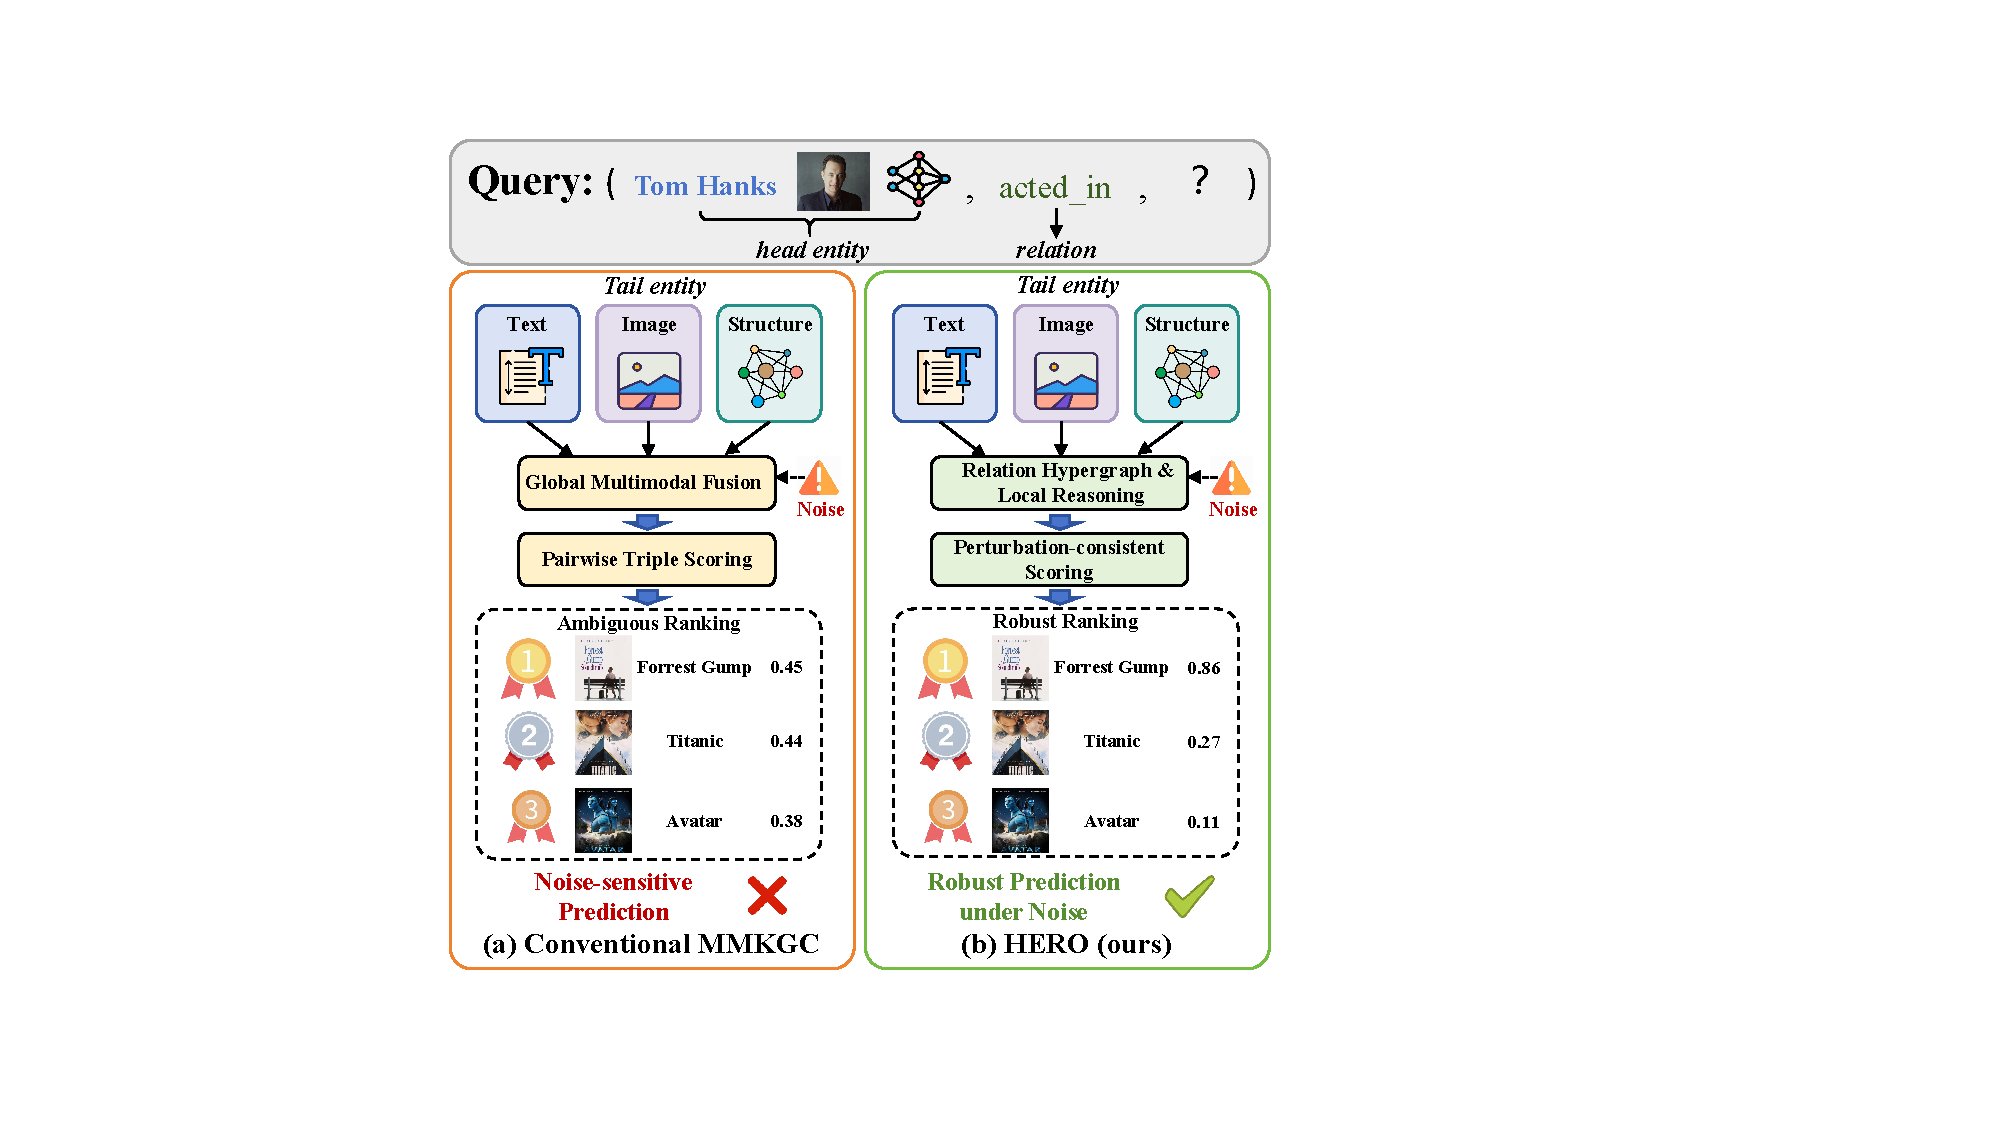
\includegraphics[width=9cm,height=9cm]{example.pdf}
    \caption{Motivation of HERO. 
    (a) Conventional MMKGC methods mainly rely on global multimodal fusion and pairwise triple scoring, which may produce ambiguous rankings with small score margins under textual, visual, or structural noise. 
    (b) HERO incorporates relation hypergraph modeling, candidate-specific local reasoning, and perturbation-consistent scoring, leading to clearer score margins and more robust prediction under noisy multimodal conditions.}
    \label{fig:intro_comparison}
\end{figure}

Motivated by these issues, we develop HERO, a hypergraph-enhanced relation-aware robust reasoning framework for MMKGC. As shown in Figure~\ref{fig:intro_comparison}(b), HERO improves relation-level structural expressiveness while reducing sensitivity to noisy multimodal inputs. It first transforms each relation type into a relation-specific hyperedge, allowing entities with shared relation semantics to exchange high-order information. The learned multimodal and high-order structural representations are then refined through candidate-specific relation-aware reasoning over context-aware local subgraphs. Finally, representation- and score-level consistency constraints are imposed between clean and perturbed branches, yielding more stable score margins under textual noise, visual interference, and structural perturbations.
The main contributions of this paper are summarized as follows:

\begin{itemize}
    \item We propose HERO, a hypergraph-enhanced relation-aware robust reasoning framework for MMKGC. HERO unifies relation-level high-order structure modeling, candidate-specific local reasoning, and perturbation consistency optimization, improving both the expressiveness and robustness of multi-modal knowledge graph completion.

    \item We design a hypergraph-based multimodal pre-training mechanism that transforms relation types into relation-specific hyperedges. This mechanism explicitly captures high-order dependencies among multiple entities sharing the same relation semantics, enabling more informative entity and relation representations.

    \item We develop a target-specific relation-aware reasoning module that constructs context-aware subgraphs for candidate triples and performs entity-relation interactive message propagation, allowing the model to exploit local structural evidence closely associated with each prediction target.

    \item Experiments on multiple MMKGC benchmark datasets show consistent gains over state-of-the-art baselines. Ablation and robustness analyses further support the roles of relation hypergraph modeling, target-specific local reasoning, and perturbation consistency optimization.


\end{itemize}

The remainder of this paper is organized as follows. Section~\ref{sec:related_work} reviews related studies on traditional knowledge graph completion and multimodal knowledge graph completion. Section~\ref{sec:preliminaries} introduces the notations and task formulation used in this work. Section~\ref{sec:method} presents the proposed HERO framework. Section~\ref{sec:experiments} reports the experimental results and analysis. Finally, Section~\ref{sec:conclusion} concludes the paper and discusses future directions.

\section{Related Work}
\label{sec:related_work}
\subsection{Traditional Knowledge Graph Completion}

Knowledge graph completion (KGC) aims to infer missing facts from observed triples and has been extensively studied in knowledge representation learning. Existing KGC methods typically embed entities and relations into low-dimensional continuous spaces, and evaluate the plausibility of candidate triples through relation-specific scoring functions. According to their modeling principles, traditional KGC methods can be broadly categorized into three representative lines: distance-based models, semantic matching models, and neural network-based models.

Distance-based models interpret relations as geometric transformations between entity embeddings. TransE~\cite{bordes2013transe} is a seminal method in this category, which models a relation as a translation from the head entity to the tail entity. This simple formulation provides an efficient and scalable solution for relational representation learning, but its expressiveness is limited when modeling complex relation patterns, such as symmetry, antisymmetry, and composition. To improve the modeling capacity of geometric transformations, RotatE~\cite{sun2019rotate} represents relations as rotations in the complex vector space, enabling multiple relational patterns to be captured within a unified framework. PairRE~\cite{chao2021pairre} further introduces paired relation vectors for the head and tail entities, allowing relation-specific transformations to better adapt to diverse mapping properties.

Semantic matching models measure the plausibility of candidate triples by explicitly modeling interactions among head entities, relations, and tail entities. RESCAL~\cite{nickel2011rescal} represents each relation as a full matrix, which enables fine-grained interactions between entity dimensions, but its high parameter complexity limits scalability on large-scale KGs. DistMult~\cite{yang2015distmult} improves computational efficiency by restricting relation matrices to diagonal forms, while this simplification weakens its ability to model asymmetric relations. ComplEx~\cite{trouillon2016complex} extends bilinear matching into the complex-valued space, where asymmetric relation patterns can be captured through complex-valued interactions. TuckER~\cite{balazevic2019tucker} formulates KGC as a tensor factorization problem and adopts Tucker decomposition to model high-order interactions among entities and relations. Compared with distance-based models, semantic matching methods provide stronger interaction modeling in the scoring function, but their predictions are still mainly derived from triple-level structural patterns.

Neural network-based models further enhance KGC by introducing nonlinear feature interaction and graph-structured message propagation. SME~\cite{bordes2014sme} employs feed-forward neural networks to learn nonlinear interactions among triple components. ConvE~\cite{dettmers2018conve} and ConEx~\cite{demir2021conex} exploit convolutional operations to capture deeper feature interactions between entity and relation embeddings, thereby improving the expressive capacity of neural scoring functions. Beyond individual triple modeling, KGNN~\cite{wang2019kgnn} aggregates information from entity neighborhoods to enrich entity embeddings with local structural contexts, while KGAT~\cite{wang2019kgat} introduces attention mechanisms to distinguish the contributions of different neighboring entities and relations. By propagating information over observed graph structures, these methods improve the utilization of local relational dependencies beyond isolated triples.

Traditional KGC methods have substantially advanced structural representation learning, but they mainly rely on symbolic triples and graph connectivity. As a result, they cannot fully use auxiliary entity semantics such as descriptions and images, especially when KGs are sparse, incomplete, or ambiguous. This limitation motivates MMKGC methods that incorporate heterogeneous modalities into entity representation and missing fact inference.

\subsection{Multimodal Knowledge Graph Completion}

Multimodal knowledge graph completion (MMKGC) extends traditional KGC by incorporating heterogeneous modality information, such as textual descriptions and visual images, into knowledge representation learning. Compared with structure-only triples, multimodal information provides complementary semantic cues for entity understanding and relation inference, especially when graph structures are sparse, incomplete, or semantically ambiguous. Therefore, a central problem in MMKGC is how to align heterogeneous modality features, integrate them into effective entity representations, and exploit them for accurate missing fact prediction.

Early MMKGC studies mainly enhance structural embedding models with auxiliary textual or visual information. IKRL~\cite{xie2017ikrl} incorporates entity images into knowledge representation learning, demonstrating the complementary role of visual features for structural embeddings. TBKGC~\cite{mousselly2018tbkgc} introduces a translation-based multimodal framework to jointly exploit structural and textual information. TransAE~\cite{wang2019transae} further adopts a multimodal autoencoder to encode heterogeneous features, enabling entity representations to integrate structural and visual semantics. These methods establish the basic paradigm of multimodal enhancement, where auxiliary modality information is used to enrich entity embeddings before triple scoring. However, their modality integration strategies are usually coarse-grained, and irrelevant textual or visual signals may be introduced into the representation space.

To alleviate cross-modal discrepancy and suppress noisy modality information, subsequent studies develop more principled alignment and selective fusion mechanisms. OTKGE~\cite{cao2022otkge} formulates multimodal alignment as an optimal transport problem, reducing distributional discrepancy among heterogeneous modalities in a shared semantic space. RSME~\cite{wang2021rsme} designs a relation-aware semantic filtering mechanism to suppress irrelevant visual information according to relation semantics. MKGformer~\cite{chen2022mkgformer} adopts a hybrid Transformer with multi-level fusion to strengthen the interaction between textual and visual modalities. These methods improve multimodal representation learning by explicitly modeling cross-modal alignment or relation-conditioned modality selection. Nevertheless, most of them still produce global multimodal representations before scoring, which may be insufficient to capture candidate-specific structural evidence and may remain sensitive to noisy modality signals.

Another line of research emphasizes preserving modality-specific information during multimodal reasoning. MoSE~\cite{zhao2022mose} separates modality-specific learning and combines predictions through ensemble inference, reducing the risk of losing independent modality characteristics during fusion. IMF~\cite{li2023imf} introduces interactive multimodal fusion to model correlations among different modalities for link prediction. More recently, M-Hyper~\cite{liu2026mhyper} revisits the limitations of fusion-based and ensemble-based paradigms, and represents both independent and fused modalities in a hypercomplex space to promote collaboration between modality-specific and joint representations. These studies indicate that multimodal information should not be collapsed into a single uniform signal, since the contribution of each modality may vary across relations and inference contexts.

Recent studies further improve MMKGC by exploring adaptive fusion, fine-grained modality modeling, and structure-aware representation learning. AdaMF-MAT~\cite{zhang2024adamfmat} adaptively estimates modality importance and employs modality-adversarial training to handle imbalanced modality information. MyGO~\cite{zhang2025mygo} discretizes raw multimodal information into fine-grained tokens and performs hierarchical triple modeling, improving the utilization of detailed modality semantics. NativE~\cite{zhang2024native} investigates MMKGC in open and noisy environments, emphasizing adaptive fusion under incomplete and diverse modality conditions. SAFER~\cite{li2026safer} constructs modality-specific subgraphs and combines subgraph-aware adaptive fusion with hierarchical relation modeling, thereby preserving structural dependencies and relation semantics across different granularities. These methods show that effective MMKGC requires not only multimodal semantic fusion, but also relation-aware and structure-aware representation learning.

Robust optimization and negative sampling have also been explored for discriminative MMKGC training. MMRNS~\cite{xu2022rens} constructs relation-enhanced multimodal negative samples, while MANS~\cite{zhang2023mans} introduces modality-aware negative sampling. DHNS~\cite{niu2025dhns} uses diffusion-based hierarchical sampling to generate graph- and modality-aware negatives. ComCon~\cite{chen2026comcon} decomposes multimodal representations into complementary and contradictory components and reweights negative samples, and HFR-MKGC~\cite{wang2026hfr} combines hierarchical fusion with MLLM-assisted reasoning for candidate generation and hard negative construction. These studies suggest that robust MMKGC requires expressive multimodal representations, informative supervision, and stable optimization under noisy or incomplete modalities.

Despite these advances, existing multimodal knowledge concept recognition (MMKGC) methods still face two key challenges. First, most methods represent structural facts as independent pairwise edges, which limits their ability to capture relation-level high-order dependencies among multiple entities sharing the same relation semantics. Second, although multimodal fusion and neighborhood-based reasoning improve entity representation learning, representation propagation and triple scoring are rarely regularized from the perspective of perturbation stability, making candidate fact prediction sensitive to modality noise and structural perturbations. Different from existing methods, HERO introduces relation hypergraph modeling to explicitly organize multi-entity dependencies under shared relation semantics, and further combines context-aware local reasoning with perturbation consistency optimization to enhance both structural expressiveness and noise-stable reasoning for MMKGC.

\section{Preliminaries}
\label{sec:preliminaries}
This section introduces the notations and task formulation used throughout this paper. The main symbols are summarized in Table~\ref{tab:notations}.


\begin{table}[t]
\centering
\caption{Summary of key notations.}
\label{tab:notations}
\begin{tabular}{ll}
\toprule
\textbf{Notation} & \textbf{Description} \\
\midrule
$\mathcal{G}$ & Multimodal knowledge graph \\
$\mathcal{E}$ & Entity set \\
$\mathcal{R}$ & Relation set \\
$\mathcal{T}$ & Structural triple set \\
$\mathcal{M}$ & Auxiliary modality information \\
$(h,r,t)$ & Triple with head entity $h$, relation $r$, and tail entity $t$ \\
$\tau$ & Candidate triple, where $\tau=(h,r,t)$ \\
$d_i$ & Textual description of entity $e_i$ \\
$I_i$ & Visual image of entity $e_i$ \\
$\mathcal{H}$ & Relation hypergraph \\
$\varepsilon_r$ & Relation-specific hyperedge corresponding to relation $r$ \\
$\mathbf{H}$ & Incidence matrix of the relation hypergraph \\
$\mathbf{Z}_{e}$ & Entity embedding matrix \\
$\mathbf{Z}_{r}$ & Relation embedding matrix \\
$\mathcal{G}_{\tau}$ & Context-aware subgraph for candidate triple $\tau$ \\
$\mathcal{V}_{\tau}$ & Node set of $\mathcal{G}_{\tau}$ \\
$\mathcal{A}_{\tau}$ & Relation edge set of $\mathcal{G}_{\tau}$ \\
$\mathcal{T}^{+}$ & Positive triple set \\
$\mathcal{T}^{-}$ & Negative triple set \\
\bottomrule
\end{tabular}
\end{table}

\paragraph{Definition 3.1 (Knowledge Graph).}
A knowledge graph (KG) represents factual knowledge as a set of relational triples. Formally, a KG is denoted as $\mathcal{G}_{s}=(\mathcal{E},\mathcal{R},\mathcal{T})$, where $\mathcal{E}$, $\mathcal{R}$, and $\mathcal{T}$ denote the entity set, relation set, and structural triple set, respectively. Each triple $(h,r,t)\in\mathcal{T}$ describes a relation $r\in\mathcal{R}$ from the head entity $h\in\mathcal{E}$ to the tail entity $t\in\mathcal{E}$. In conventional KGs, each structural fact is usually represented as a pairwise relational edge between two entities, which provides the basic structural input for knowledge graph completion.

\paragraph{Definition 3.2 (Knowledge Graph Completion).}
Knowledge graph completion (KGC) aims to infer missing facts from observed triples. Given an incomplete query $(h,r,?)$ or $(?,r,t)$, the objective is to rank candidate entities in $\mathcal{E}$ and identify the most plausible missing tail or head entity. A KGC model generally learns entity and relation representations and defines a scoring function $s(h,r,t)$ to measure the plausibility of each candidate triple. A higher score indicates stronger semantic compatibility among the head entity, relation, and tail entity.

During training, observed triples are regarded as positive triples and denoted as $\mathcal{T}^{+}$. Negative triples are usually constructed by replacing the head or tail entity of positive triples, forming the negative triple set $\mathcal{T}^{-}$. The training set is therefore denoted as $\mathcal{D}=\mathcal{T}^{+}\cup\mathcal{T}^{-}$. The model is optimized to assign higher scores to positive triples than to negative triples, thereby learning discriminative representations for missing fact prediction.

\paragraph{Definition 3.3 (Multimodal Knowledge Graph).}
A multimodal knowledge graph (MMKG) extends a conventional KG by associating entities with heterogeneous modality information. In this paper, an MMKG is formally defined as
$\mathcal{G}=(\mathcal{E},\mathcal{R},\mathcal{T},\mathcal{M})$,
where $\mathcal{E}$, $\mathcal{R}$, and $\mathcal{T}$ denote the entity set, relation set, and structural triple set, respectively. $\mathcal{M}$ denotes the auxiliary modality information associated with entities, mainly including textual descriptions and visual images. For each entity $e_i\in\mathcal{E}$, its textual description and visual image are denoted as $d_i$ and $I_i$, respectively. In this work, such multimodal information provides complementary semantic cues for entity representation learning, while structural triples provide relational evidence for fact inference.

\paragraph{Definition 3.4 (Multimodal Knowledge Graph Completion).}
Given an MMKG $\mathcal{G}=(\mathcal{E},\mathcal{R},\mathcal{T},\mathcal{M})$, multimodal knowledge graph completion (MMKGC) aims to predict the missing entity for a query $(h,r,?)$ or $(?,r,t)$ by ranking candidate entities in $\mathcal{E}$. For a candidate triple $\tau=(h,r,t)$, the model computes a plausibility score to determine whether the triple is likely to be valid. Compared with traditional KGC, MMKGC exploits both structural triples and multimodal entity information, which is particularly beneficial when graph structures are sparse, incomplete, or semantically ambiguous.


\section{Method}
\label{sec:method}
MMKGC aims to infer missing facts by jointly exploiting structural triples and auxiliary modality information, such as textual descriptions and visual images. Although existing methods have achieved promising progress through multimodal fusion and neighborhood-based reasoning, two limitations remain insufficiently addressed. First, conventional pairwise edge structures mainly describe local associations between entity pairs, making it difficult to capture relation-level high-order dependencies among multiple entities sharing the same relation semantics. Second, candidate fact prediction requires both target-specific structural evidence and robustness against multimodal noise and structural perturbations. Directly relying on global representations may overlook local evidence closely related to the candidate triple, while noisy textual descriptions, irrelevant visual backgrounds, and incomplete structural connections may lead to unstable representation propagation and unreliable triple scoring.

\begin{figure*}[t]
    \centering
    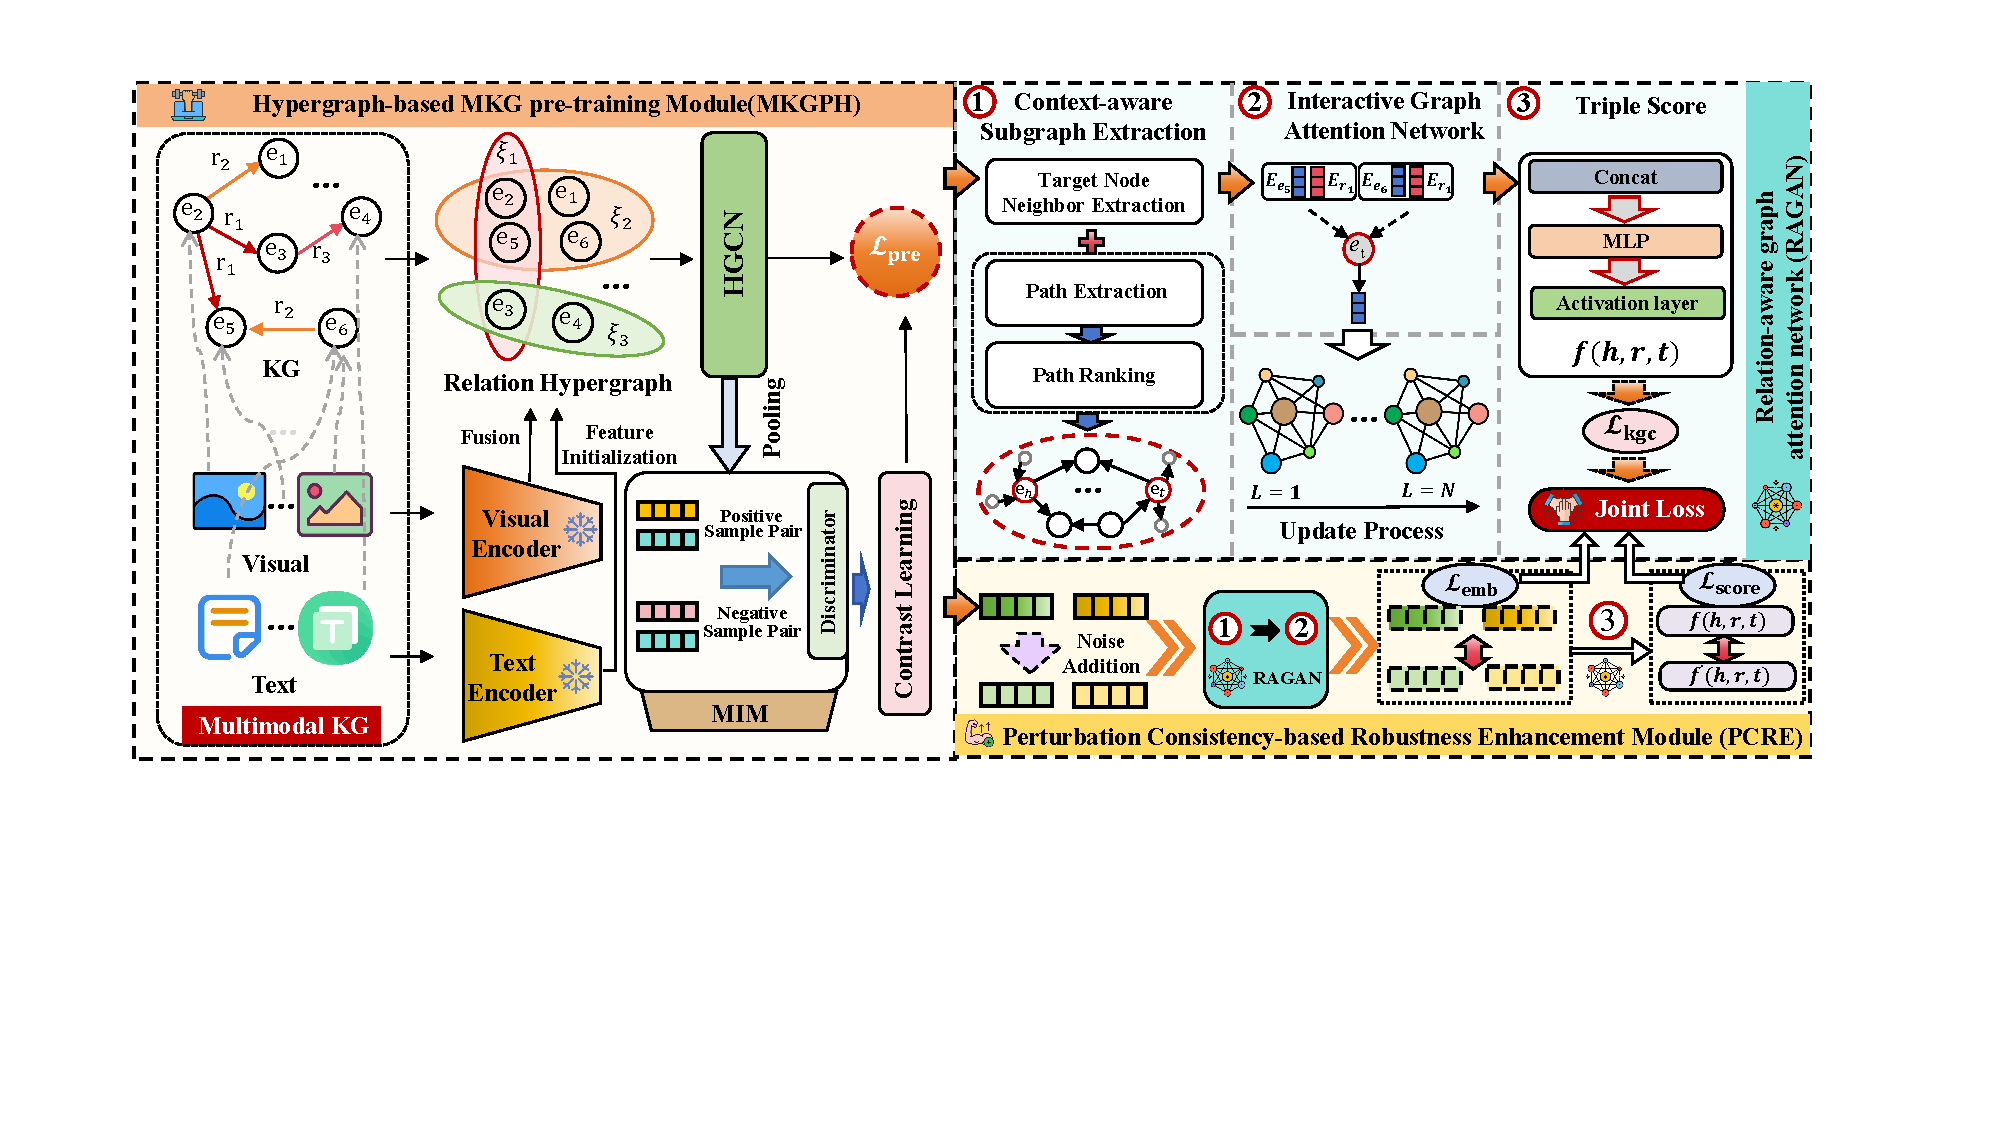
\includegraphics[width=0.95\textwidth]{model.pdf}
    \caption{Overall architecture of HERO. The framework first employs hypergraph-based MKG pre-training to integrate textual, visual, and relation-level high-order structural information into entity and relation embeddings. For each candidate triple, a context-aware subgraph is constructed and encoded by a relation-aware graph attention network to capture target-specific local structural evidence. To improve robustness, perturbations are introduced into entity and relation embeddings, and consistency constraints are imposed at both the representation and score levels between clean and perturbed branches.}
    \label{fig:overall_framework}
\end{figure*}

Figure~\ref{fig:overall_framework} shows the architecture of HERO. The framework contains three components. A hypergraph-based multimodal knowledge graph pre-training module first builds a relation hypergraph and learns entity and relation representations that combine textual, visual, and high-order relational information. For each candidate triple, HERO then extracts a context-aware subgraph and encodes it with a relation-aware graph attention network to capture target-specific local evidence. Finally, a perturbation consistency module constrains clean and perturbed branches at both the embedding and score levels, improving prediction stability under noisy multimodal conditions.

\subsection{Hypergraph-based MKG Pre-training Module}

HERO uses a hypergraph-based multimodal knowledge graph pre-training module, termed MKGPH, to move beyond pairwise structural modeling. MKGPH transforms relation types into relation-specific hyperedges, so entities involved in the same relation are propagated as high-order semantic groups rather than isolated pairwise triples. The resulting entity and relation embeddings initialize the subsequent candidate-specific reasoning module.

MKGPH consists of four main steps. It first encodes textual and visual modalities into unified entity representations. It then constructs a relation hypergraph from structural triples, where each hyperedge corresponds to one relation type. Based on the constructed hypergraph, hypergraph convolution is performed to propagate information between entity nodes and relation hyperedges. Finally, MKGPH is optimized by combining a triple discrimination objective and a hyperedge-level mutual information maximization objective, enabling the learned representations to capture multimodal semantics, relation-level high-order structures, and fact-level discrimination signals.

\subsubsection{Multimodal Entity Encoding}

Entities in MMKGs are usually associated with heterogeneous modality information. Textual descriptions provide semantic cues such as category, attribute, and contextual information, while visual images offer complementary information related to appearance, scenes, and visual characteristics. To obtain unified entity features for subsequent hypergraph propagation, MKGPH first encodes textual and visual modalities separately and then projects them into a shared semantic space.

Given a multimodal knowledge graph $\mathcal{G}=(\mathcal{E},\mathcal{R},\mathcal{T},\mathcal{M})$, where $\mathcal{E}$ denotes the entity set, $\mathcal{R}$ denotes the relation set, $\mathcal{T}=\{(h,r,t)\mid h,t\in\mathcal{E},r\in\mathcal{R}\}$ denotes the structural triple set, and $\mathcal{M}$ denotes the auxiliary modality information. For each entity $e_i\in\mathcal{E}$, its textual description and visual image are denoted as $d_i$ and $I_i$, respectively.

For textual and visual modalities, BERT and ViT are adopted as modality encoders to obtain the textual representation $\mathbf{x}_i^{t}\in\mathbb{R}^{d_t}$ and the visual representation $\mathbf{x}_i^{v}\in\mathbb{R}^{d_v}$:
\begin{equation}
\left\{
\begin{aligned}
\mathbf{x}_i^{t} &= \mathrm{BERT}(d_i), \\
\mathbf{x}_i^{v} &= \mathrm{ViT}(I_i).
\end{aligned}
\right.
\end{equation}

Since textual and visual representations have different feature dimensions and semantic distributions, directly using them for graph propagation may introduce modality-space inconsistency. Therefore, the two modality representations are concatenated and projected into a common embedding space:
\begin{equation}
\mathbf{x}_i^{0}
=
\phi
\left(
\mathbf{W}_{m}
\left[
\mathbf{x}_i^{t}
\Vert
\mathbf{x}_i^{v}
\right]
+
\mathbf{b}_{m}
\right),
\end{equation}
where $\Vert$ denotes vector concatenation, $\mathbf{W}_{m}\in\mathbb{R}^{d\times(d_t+d_v)}$ and $\mathbf{b}_{m}\in\mathbb{R}^{d}$ are learnable parameters, and $\phi(\cdot)$ denotes the ReLU activation function. The output $\mathbf{x}_i^{0}\in\mathbb{R}^{d}$ is the initial multimodal embedding of entity $e_i$. The initial embeddings of all entities are stacked row-wise to form the node feature matrix:
\begin{equation}
\mathbf{X}^{0}
=
[\mathbf{x}_1^{0},\mathbf{x}_2^{0},\ldots,\mathbf{x}_{|\mathcal{E}|}^{0}]^{\top}
\in
\mathbb{R}^{|\mathcal{E}|\times d}.
\end{equation}
This process aligns textual and visual semantics at the entity-node level and provides consistent node features for relation hypergraph propagation.

\begin{figure}[t]
    \centering
    \subfigure[Traditional knowledge graph]{
        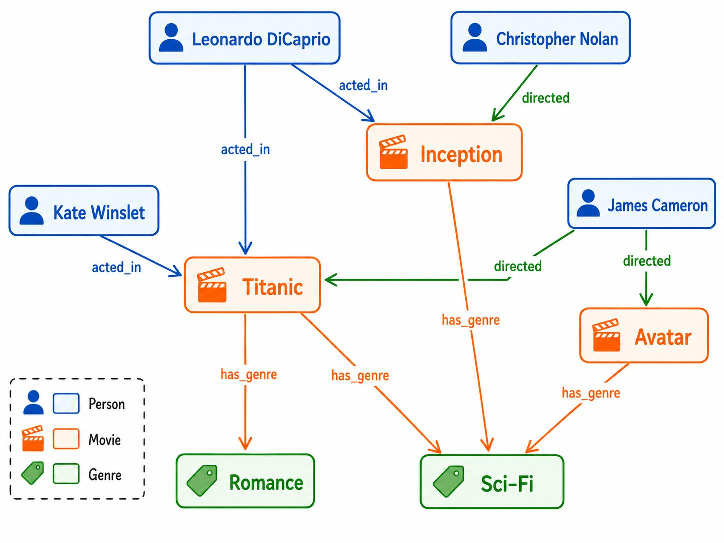
\includegraphics[width=6cm,height=4cm]{kg_lefts3.pdf}
    }
    \subfigure[Relation hypergraph]{
        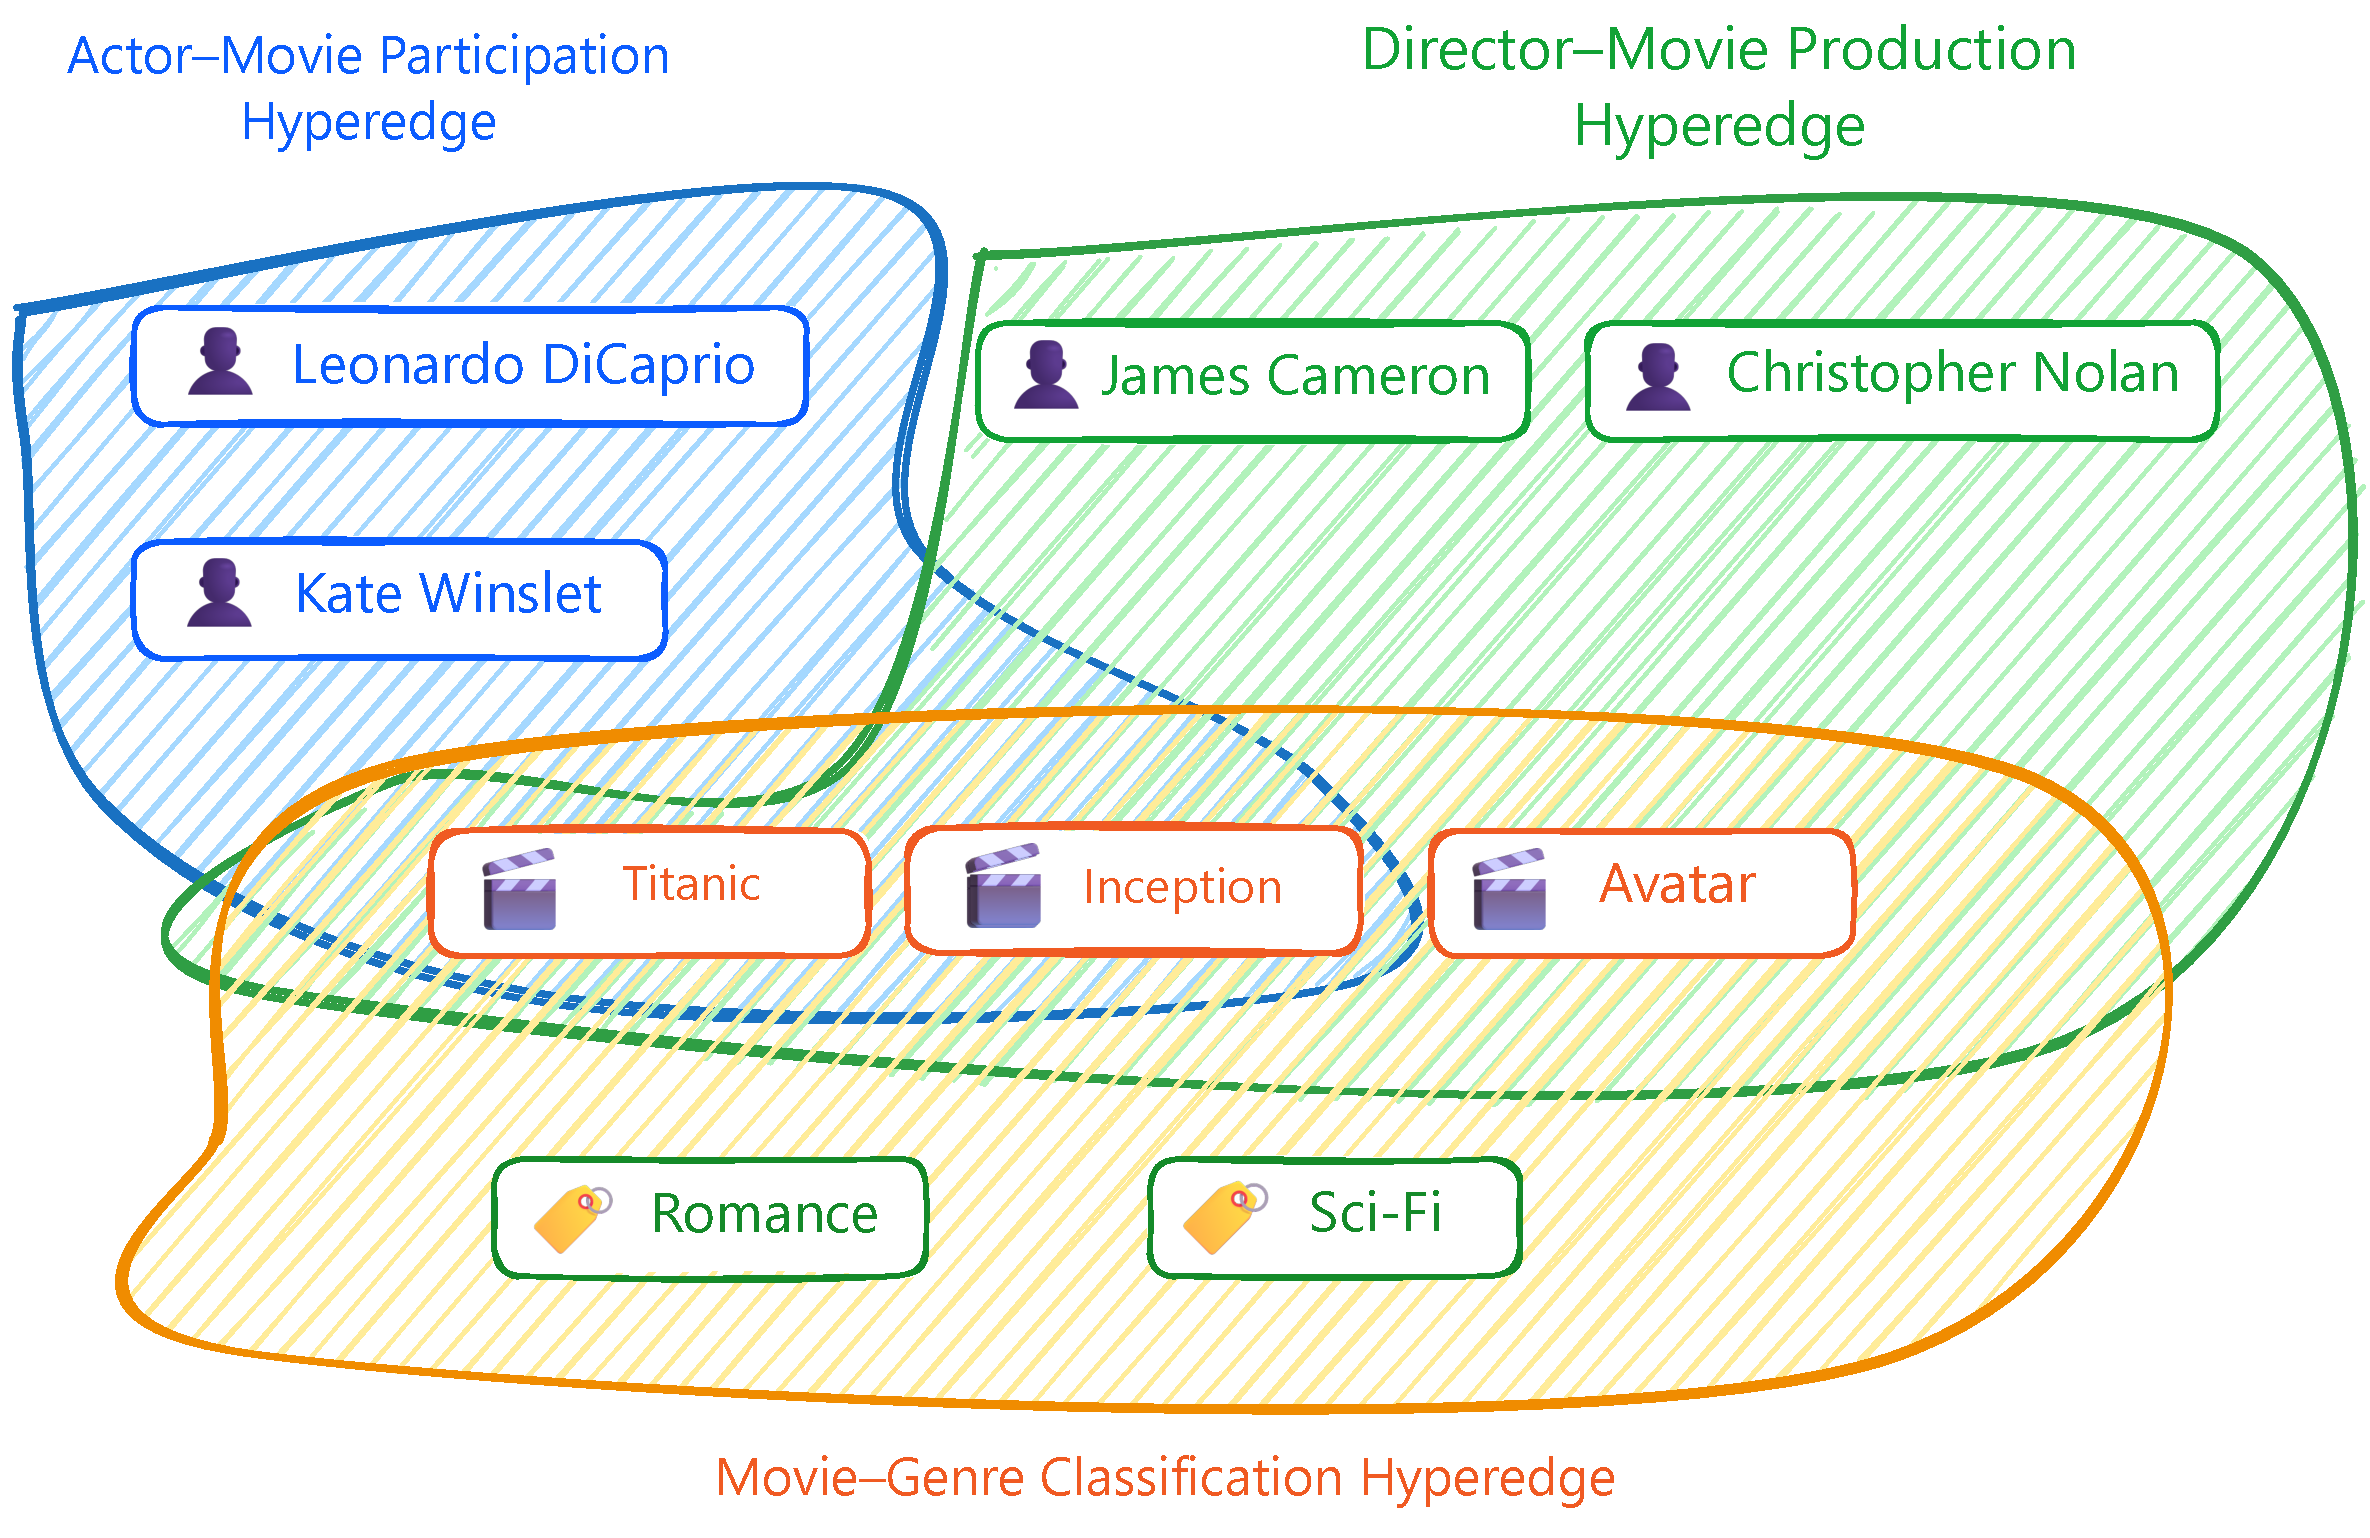
\includegraphics[width=6cm,height=4cm]{hp_right4.pdf}
    }
    \caption{Illustration of transforming a traditional knowledge graph into a relation hypergraph. The traditional knowledge graph represents facts as pairwise relational edges, while the relation hypergraph maps each relation type to a relation-specific hyperedge connecting all entities involved in that relation. This transformation enables the model to aggregate and redistribute information among multiple entities sharing the same relation semantics.}
    \label{hypergraph_mot}
\end{figure}

\subsubsection{Relation Hypergraph Construction}

Structural triples provide explicit relational evidence for MMKGC. However, conventional KGs represent each fact as a pairwise edge between a head entity and a tail entity. Such a representation is effective for modeling local entity-pair associations, but it is insufficient to capture high-order dependencies among multiple entities involved in the same relation type. For example, entities participating in the same relation often form a relation-specific semantic group, and their collective participation patterns cannot be fully represented by isolated pairwise edges.

MKGPH converts the original structural triples into a relation hypergraph. As shown in Figure~\ref{hypergraph_mot}, each relation type is mapped to a relation-specific hyperedge that connects all entities involved in that relation. Facts scattered across multiple triples are therefore organized into relation-level entity groups, enabling node-to-hyperedge-to-node information propagation.

Formally, the relation hypergraph is defined as $\mathcal{H}=(\mathcal{V},\mathcal{E}_{h})$, where $\mathcal{V}=\mathcal{E}$ denotes the hypergraph node set and $\mathcal{E}_{h}$ denotes the relation hyperedge set. For each relation $r\in\mathcal{R}$, its corresponding hyperedge $\varepsilon_r$ is defined as:
\begin{equation}
\varepsilon_r
=
\left\{
e_i\in\mathcal{E}
\mid
\exists e_j\in\mathcal{E},
(e_i,r,e_j)\in\mathcal{T}
\ \mathrm{or}\
(e_j,r,e_i)\in\mathcal{T}
\right\}.
\end{equation}
Accordingly, the hyperedge set is given by $\mathcal{E}_{h}=\{\varepsilon_r\mid r\in\mathcal{R}\}$. This definition treats each relation as a semantic unit and aggregates all entities participating in that relation into a shared hyperedge, thereby providing a structural basis for relation-level high-order dependency modeling.

To support hypergraph convolution, an incidence matrix $\mathbf{H}\in\mathbb{R}^{|\mathcal{E}|\times|\mathcal{R}|}$ is constructed to describe the membership between entity nodes and relation hyperedges:
\begin{equation}
\mathbf{H}_{ir}
=
\begin{cases}
1, & e_i\in\varepsilon_r, \\
0, & e_i\notin\varepsilon_r.
\end{cases}
\end{equation}
Here, the $i$-th row corresponds to entity $e_i$, and the $r$-th column corresponds to relation hyperedge $\varepsilon_r$. The incidence matrix converts entity-relation participation in the original KG into node-hyperedge membership relations.

Since entities and relation hyperedges may have different connection scales, direct propagation over $\mathbf{H}$ may bias representation learning toward highly connected entities or large hyperedges. Therefore, we define the node degree matrix $\mathbf{D}_{v}\in\mathbb{R}^{|\mathcal{E}|\times|\mathcal{E}|}$ and the hyperedge degree matrix $\mathbf{D}_{e}\in\mathbb{R}^{|\mathcal{R}|\times|\mathcal{R}|}$ as:
\begin{equation}
\left\{
\begin{aligned}
\mathbf{D}_{v}(i,i) 
&= 
\sum_{r=1}^{|\mathcal{R}|}\mathbf{H}_{ir}, \\
\mathbf{D}_{e}(r,r) 
&= 
\sum_{i=1}^{|\mathcal{E}|}\mathbf{H}_{ir}.
\end{aligned}
\right.
\end{equation}
Here, $\mathbf{D}_{v}(i,i)$ denotes the number of relation hyperedges involving entity $e_i$, and $\mathbf{D}_{e}(r,r)$ denotes the number of entities contained in relation hyperedge $\varepsilon_r$. These matrices are used to normalize node and hyperedge contributions during hypergraph convolution.

\subsubsection{Hypergraph Convolutional Network}

After constructing the relation hypergraph, MKGPH employs a hypergraph convolutional network to encode relation-level high-order semantics into entity representations. Different from ordinary graph convolution, which aggregates information along pairwise edges, hypergraph convolution follows a node-to-hyperedge-to-node propagation mechanism. Entity representations are first aggregated into relation hyperedges, and then the relation-level information is propagated back to related entity nodes. In this way, entities sharing the same relation semantics can exchange information through their common hyperedge.

The $l$-th hypergraph convolution layer is defined as:
\begin{equation}
\mathbf{X}^{l+1}
=
\phi
\left(
\mathbf{D}_{v}^{-\frac{1}{2}}
\mathbf{H}
\mathbf{D}_{e}^{-1}
\mathbf{H}^{\top}
\mathbf{D}_{v}^{-\frac{1}{2}}
\mathbf{X}^{l}
\mathbf{W}^{l}
\right),
\end{equation}
where $\mathbf{X}^{l}\in\mathbb{R}^{|\mathcal{E}|\times d_l}$ denotes the entity representations at the $l$-th layer, $\mathbf{W}^{l}\in\mathbb{R}^{d_l\times d_{l+1}}$ is a learnable transformation matrix, and $\phi(\cdot)$ is the ReLU activation function.

In this propagation process, $\mathbf{H}^{\top}$ aggregates entity node representations into their associated relation hyperedges, while $\mathbf{D}_{e}^{-1}$ normalizes the contributions of entities within each hyperedge. Then, $\mathbf{H}$ propagates hyperedge representations back to related entity nodes, and $\mathbf{D}_{v}^{-\frac{1}{2}}$ normalizes differences in the number of hyperedges associated with each entity. Through multi-layer propagation, MKGPH progressively enhances entity representations with relation-level high-order structural information.

After $L$ layers, the entity embedding matrix is obtained as:
\begin{equation}
\mathbf{Z}_{e}=\mathbf{X}^{L}\in\mathbb{R}^{|\mathcal{E}|\times d},
\end{equation}
where the embedding of entity $e_i$ is denoted as $\mathbf{z}_i=\mathbf{Z}_{e}[i]\in\mathbb{R}^{d}$. Each entity embedding encodes both multimodal semantic information and high-order relational information propagated from the relation hypergraph.

Since each relation is represented as a hyperedge connecting multiple entities, the relation embedding is derived by aggregating the embeddings of entities within the corresponding hyperedge:
\begin{equation}
\mathbf{z}_r
=
\frac{1}{|\varepsilon_r|}
\sum_{e_i\in\varepsilon_r}
\mathbf{z}_i.
\end{equation}
In matrix form, all relation embeddings are computed as:
\begin{equation}
\mathbf{Z}_{r}
=
\mathbf{D}_{e}^{-1}
\mathbf{H}^{\top}
\mathbf{Z}_{e}
\in
\mathbb{R}^{|\mathcal{R}|\times d}.
\end{equation}
Here, $\mathbf{Z}_{r}[r]=\mathbf{z}_r$ denotes the representation of relation $r$. This aggregation allows relation embeddings to reflect the overall semantic distribution of entities participating in the corresponding relation, thereby providing relation-level representations for downstream reasoning.

\subsubsection{Triple Scoring}

Although hypergraph convolution captures multimodal and relation-level high-order information, the learned representations still need to be optimized for fact discrimination. Therefore, MKGPH introduces a triple scoring mechanism to distinguish observed triples from negative sampled triples.

For a candidate triple $(h,r,t)$, the head entity, relation, and tail entity representations are denoted as $\mathbf{z}_{h}$, $\mathbf{z}_{r}$, and $\mathbf{z}_{t}$, respectively. To preserve the individual semantics of triple components and explicitly model their pairwise interactions, the triple interaction representation is constructed as:
\begin{equation}
\mathbf{u}_{h,r,t}
=
\left[
\mathbf{z}_{h}
\Vert
\mathbf{z}_{r}
\Vert
\mathbf{z}_{t}
\Vert
(\mathbf{z}_{h}\odot\mathbf{z}_{r})
\Vert
(\mathbf{z}_{r}\odot\mathbf{z}_{t})
\Vert
(\mathbf{z}_{h}\odot\mathbf{z}_{t})
\right],
\end{equation}
where $\Vert$ denotes concatenation and $\odot$ denotes element-wise multiplication. The concatenation terms retain the original representations, while the element-wise products capture local interaction patterns among the head entity, relation, and tail entity.

Given $\mathbf{u}_{h,r,t}$, the plausibility score of the candidate triple is computed by a two-layer nonlinear scoring function:
\begin{equation}
s_{HT}(h,r,t)
=
\mathbf{w}_{2}^{\top}
\phi
\left(
\mathbf{W}_{1}\mathbf{u}_{h,r,t}
+
\mathbf{b}_{1}
\right)
+
b_{2},
\end{equation}
where $\mathbf{W}_{1}$ and $\mathbf{b}_{1}$ are the hidden-layer parameters, $\mathbf{w}_{2}$ and $b_{2}$ are the output-layer parameters, and $\phi(\cdot)$ denotes the ReLU activation function. A higher score indicates stronger compatibility among the head entity, relation, and tail entity.

To optimize triple discrimination, negative triples $\mathcal{T}^{-}$ are generated by randomly corrupting the head or tail entity of positive triples $\mathcal{T}^{+}$. The binary cross-entropy loss is defined as:
\begin{equation}
\mathcal{L}_{HT}
=
-\sum_{(h,r,t)\in\mathcal{T}^{+}}
\log
\sigma
\left(
s_{HT}(h,r,t)
\right)
-
\sum_{(h',r,t')\in\mathcal{T}^{-}}
\log
\left(
1-
\sigma
\left(
s_{HT}(h',r,t')
\right)
\right),
\end{equation}
where $\sigma(\cdot)$ is the sigmoid function, and $(h',r,t')$ denotes a negative sampled triple. By assigning higher scores to positive triples and lower scores to negative triples, $\mathcal{L}_{HT}$ encourages the hypergraph-encoded embeddings to form a fact-discriminative representation space.

\subsubsection{Mutual Information Maximization}

The triple discrimination loss supervises embeddings at the fact level, but it mainly focuses on the plausibility of individual triples. Since MKGPH organizes entities into relation-specific hyperedges, it is also necessary to preserve the semantic consistency of entity combinations within each hyperedge. To this end, MKGPH introduces a hyperedge-level mutual information maximization objective, which contrasts real relation hyperedges with perturbed hyperedges.

For a real hyperedge $\varepsilon_r$, a perturbed hyperedge $\widetilde{\varepsilon}_r$ is constructed by randomly replacing a subset of entities in $\varepsilon_r$ with entities sampled from $\mathcal{E}\setminus\varepsilon_r$. The representations of the real and perturbed hyperedges are computed as:
\begin{equation}
\left\{
\begin{aligned}
\mathbf{z}_{\varepsilon_r}
&=
\frac{1}{|\varepsilon_r|}
\sum_{e_i\in\varepsilon_r}
\mathbf{z}_i, \\
\widetilde{\mathbf{z}}_{\varepsilon_r}
&=
\frac{1}{|\widetilde{\varepsilon}_r|}
\sum_{e_i\in\widetilde{\varepsilon}_r}
\mathbf{z}_i.
\end{aligned}
\right.
\end{equation}
The real hyperedge preserves the original relation-specific entity combination, whereas the perturbed hyperedge disrupts this high-order structure. Thus, they serve as positive and negative hyperedge samples for contrastive learning.

To provide a global semantic reference, the representations of all real relation hyperedges are averaged and transformed as:
\begin{equation}
\mathbf{g}
=
\phi
\left(
\mathbf{W}_{g}
\left(
\frac{1}{|\mathcal{R}|}
\sum_{r=1}^{|\mathcal{R}|}
\mathbf{z}_{\varepsilon_r}
\right)
+
\mathbf{b}_{g}
\right),
\end{equation}
where $\mathbf{W}_{g}$ and $\mathbf{b}_{g}$ are learnable parameters. The global representation $\mathbf{g}$ summarizes the overall semantic distribution of relation hyperedges.

A bilinear discriminator is then used to measure the matching probability between a hyperedge representation and the global representation:
\begin{equation}
D(\mathbf{z},\mathbf{g})
=
\sigma
\left(
\mathbf{z}^{\top}
\mathbf{W}_{D}
\mathbf{g}
\right),
\end{equation}
where $\mathbf{W}_{D}\in\mathbb{R}^{d\times d}$ is a learnable parameter matrix.

The hyperedge-level contrastive loss is defined as:
\begin{equation}
\mathcal{L}_{CL}
=
-\sum_{r=1}^{|\mathcal{R}|}
\left[
\log
D
\left(
\mathbf{z}_{\varepsilon_r},
\mathbf{g}
\right)
+
\log
\left(
1-
D
\left(
\widetilde{\mathbf{z}}_{\varepsilon_r},
\mathbf{g}
\right)
\right)
\right].
\end{equation}
This objective increases the consistency between real hyperedge representations and the global relation-hypergraph representation, while reducing the matching probability of perturbed hyperedges. Different from $\mathcal{L}_{HT}$, which emphasizes fact-level discrimination, $\mathcal{L}_{CL}$ regularizes hyperedge-level semantic consistency and further strengthens relation-level high-order representation learning. 

\subsubsection{Overall Pre-training Objective}

The overall pre-training objective of MKGPH jointly optimizes the triple discrimination loss and the hyperedge-level contrastive loss:
\begin{equation}
\mathcal{L}_{pre}
=
\mathcal{L}_{HT}
+
\lambda_{CL}\mathcal{L}_{CL},
\end{equation}
where $\lambda_{CL}$ is a balancing coefficient. By minimizing $\mathcal{L}_{pre}$, MKGPH learns entity and relation representations that integrate multimodal semantics, relation-level high-order structures, and fact-level discrimination signals. The obtained entity embedding matrix $\mathbf{Z}_{e}$ and relation embedding matrix $\mathbf{Z}_{r}$ are used as the initialization for subsequent relation-aware reasoning. The complete pre-training procedure of MKGPH is summarized in Algorithm~\ref{alg:mkgph}.

\begin{algorithm}[t]
\caption{Pre-training Procedure of MKGPH}
\label{alg:mkgph}
\begin{algorithmic}[1]

\REQUIRE \ \\
Multimodal knowledge graph $\mathcal{G}=(\mathcal{E},\mathcal{R},\mathcal{T},\mathcal{M})$;\\
Entity set $\mathcal{E}$, relation set $\mathcal{R}$, triple set $\mathcal{T}$, multimodal information $\mathcal{M}$;\\
Balance coefficient $\lambda_{CL}$;\\
Text encoder BERT and visual encoder ViT;\\
Learnable parameters $\Theta_{mkgph}$;

\ENSURE \ \\
Entity embeddings $\mathbf{Z}_{e}$;\\
Relation embeddings $\mathbf{Z}_{r}$;\\
Trained parameters $\Theta_{mkgph}$;

\STATE Encode textual and visual information of each entity with BERT and ViT;
\STATE Project multimodal features into a shared embedding space to obtain initial entity features $\mathbf{X}^{0}$;
\STATE Construct relation hyperedges $\{\varepsilon_r\}_{r\in\mathcal{R}}$ from structural triples in $\mathcal{T}$;
\STATE Build the relation hypergraph $\mathcal{H}=(\mathcal{V},\mathcal{E}_{h})$;
\STATE Construct incidence matrix $\mathbf{H}$ for the relation hypergraph;

\STATE \textbf{For} {each training epoch} \textbf{do}

    \STATE \hspace{0.5cm} Perform hypergraph convolution over $\mathcal{H}$ to obtain entity embeddings $\mathbf{Z}_{e}$;
    \STATE \hspace{0.5cm} Aggregate entity embeddings within each relation hyperedge to obtain relation embeddings $\mathbf{Z}_{r}$;
    \STATE \hspace{0.5cm} Sample negative triples by randomly corrupting positive triples in $\mathcal{T}$;
    \STATE \hspace{0.5cm} Compute the triple discrimination loss $\mathcal{L}_{HT}$;
    \STATE \hspace{0.5cm} Construct perturbed hyperedges for contrastive learning;
    \STATE \hspace{0.5cm} Compute the hyperedge-level contrastive loss $\mathcal{L}_{CL}$;
    \STATE \hspace{0.5cm} Optimize $\mathcal{L}_{pre}=\mathcal{L}_{HT}+\lambda_{CL}\mathcal{L}_{CL}$;
    \STATE \hspace{0.5cm} Update $\Theta_{mkgph}$ by minimizing $\mathcal{L}_{pre}$ with gradient descent;

\STATE \textbf{End For} \\
\STATE \textbf{Return} $\mathbf{Z}_{e}$, $\mathbf{Z}_{r}$, and updated $\Theta_{mkgph}$

\end{algorithmic}
\end{algorithm}


\subsection{Relation-aware Graph Attention Network}

The MKGPH module learns entity and relation embeddings by integrating multimodal semantics and relation-level high-order structural information through relation hypergraph pre-training. However, these representations are mainly obtained from the global hypergraph structure and are not explicitly conditioned on a specific candidate triple $\tau=(h,r,t)$. For MMKGC, the validity of a candidate triple depends not only on the global compatibility among the head entity, relation, and tail entity, but also on target-specific local evidence, such as the neighborhoods around the target entities, the multi-hop connection patterns between them, and the relation semantics along these paths. Therefore, directly scoring candidate triples with global pre-trained embeddings may overlook discriminative structural evidence closely associated with the current prediction target.

HERO employs a Relation-aware Graph Attention Network, termed RAGAN, for target-triple-conditioned local reasoning. Given a candidate triple $\tau=(h,r,t)$, RAGAN constructs a context-aware subgraph from dual-end neighborhoods and semantically relevant multi-hop paths. It then performs entity-relation interactive attention propagation, where neighboring entities and adjacent relations are jointly modeled under the candidate triple condition. The plausibility score is computed from the context-enhanced head and tail representations together with the target relation representation. This design restricts message propagation to evidence relevant to the candidate fact and reduces interference from irrelevant neighborhoods.

\subsubsection{Context-aware Subgraph Extraction}

For a candidate triple $\tau=(h,r,t)$, using only the pre-trained embeddings of $h$, $r$, and $t$ is insufficient to exploit the local structural context associated with the candidate fact. In contrast, performing message passing over the entire knowledge graph may introduce a large amount of irrelevant entities and relations, weakening the discriminative effect of local evidence. To balance contextual sufficiency and structural relevance, RAGAN constructs a context-aware subgraph for each candidate triple, so that subsequent graph attention propagation is performed within a compact and target-relevant structural scope.

The construction starts from the local neighborhoods of the head entity $h$ and the candidate tail entity $t$. Given the structural triple set $\mathcal{T}$, the $K$-hop neighborhood of an entity $e_i\in\mathcal{E}$ is defined as
$\mathcal{N}_{K}(e_i)=\{e_j\in\mathcal{E}\mid \mathrm{dist}(e_i,e_j)\leq K\}$,
where $\mathrm{dist}(e_i,e_j)$ denotes the shortest-path distance between $e_i$ and $e_j$ in the structural knowledge graph. For $\tau=(h,r,t)$, the dual-end neighborhood node set and its induced relation edge set are defined as:
\begin{equation}
\left\{
\begin{aligned}
\mathcal{V}_{\tau}^{N}
&=
\mathcal{N}_{K}(h)
\cup
\mathcal{N}_{K}(t)
\cup
\{h,t\}, \\
\mathcal{A}_{\tau}^{N}
&=
\left\{
(e_i,r_{ij},e_j)\in\mathcal{T}
\mid
e_i,e_j\in\mathcal{V}_{\tau}^{N}
\right\}.
\end{aligned}
\right.
\end{equation}
Here, $r_{ij}\in\mathcal{R}$ denotes the relation type between entities $e_i$ and $e_j$. The dual-end neighborhood structure provides local relational evidence around the target entities for evaluating the plausibility of the candidate triple.

Although dual-end neighborhoods capture local structural distributions around $h$ and $t$, they do not explicitly characterize the connection patterns between them. In KGC, multi-hop paths between the head and tail entities often reveal latent relational associations. Therefore, RAGAN further retrieves multi-hop paths from $h$ to $t$ and selects relation-relevant paths according to their semantic consistency with the target relation $r$.

A candidate path from $h$ to $t$ is represented as
$p=(h,r_1,e_1,r_2,e_2,\ldots,r_l,t)$ with $l\leq L_p$, where $L_p$ is the maximum path length, $r_1,r_2,\ldots,r_l$ denote the relation sequence, and $e_1,e_2,\ldots,e_{l-1}$ denote intermediate entities. The relation sequence of path $p$ is denoted as $\mathcal{R}(p)=(r_1,r_2,\ldots,r_l)$. Since different paths may have different semantic relevance to the target relation, incorporating all candidate paths may introduce irrelevant structural information. RAGAN therefore filters candidate paths according to their semantic similarity to the target relation.

Specifically, the path relation sequence $\mathcal{R}(p)$ is converted into a textual sequence $c(p)$, and the textual description of relation $r$ is denoted as $c(r)$. BERT is adopted to encode them into semantic representations $\mathbf{b}_{p}=\mathrm{BERT}(c(p))$ and $\mathbf{b}_{r}=\mathrm{BERT}(c(r))$. The semantic relevance between path $p$ and target relation $r$ is computed by cosine similarity:
\begin{equation}
\gamma(p,r)
=
\frac{
\mathbf{b}_{p}^{\top}\mathbf{b}_{r}
}{
\|\mathbf{b}_{p}\|_{2}\|\mathbf{b}_{r}\|_{2}
}.
\end{equation}
Candidate paths are ranked according to $\gamma(p,r)$, and the top $K_p$ paths are selected to form the target-relation-relevant path set:
\begin{equation}
\mathcal{P}_{\tau}
=
\mathrm{TopK}_{K_p}
\left(
\left\{
p
\mid
p:h\rightsquigarrow t,\ |p|\leq L_p
\right\},
\gamma(p,r)
\right),
\end{equation}
where $p:h\rightsquigarrow t$ indicates that path $p$ connects $h$ to $t$, and $|p|$ denotes the path length. This filtering mechanism retains multi-hop paths whose relation sequences are more semantically consistent with the target relation, thereby improving the relevance of the constructed subgraph to the candidate triple.

After obtaining the dual-end neighborhoods and target-relation-relevant paths, RAGAN constructs the context-aware subgraph $\mathcal{G}_{\tau}=(\mathcal{V}_{\tau},\mathcal{A}_{\tau})$ as:
\begin{equation}
\left\{
\begin{aligned}
\mathcal{V}_{\tau}
&=
\mathcal{V}_{\tau}^{N}
\cup
\left(
\bigcup_{p\in\mathcal{P}_{\tau}}
\mathcal{V}(p)
\right), \\
\mathcal{A}_{\tau}
&=
\mathcal{A}_{\tau}^{N}
\cup
\left(
\bigcup_{p\in\mathcal{P}_{\tau}}
\mathcal{A}(p)
\right).
\end{aligned}
\right.
\end{equation}
Here, $\mathcal{V}(p)$ and $\mathcal{A}(p)$ denote the entity node set and relation edge set contained in path $p$, respectively. The resulting subgraph integrates neighborhood evidence around the target entities and multi-hop relational evidence between them, providing a compact structural context for target-triple-conditioned reasoning.

\subsubsection{Interactive Graph Attention Network}

Given the context-aware subgraph $\mathcal{G}_{\tau}=(\mathcal{V}_{\tau},\mathcal{A}_{\tau})$, RAGAN performs relation-aware information propagation to obtain target-triple-conditioned entity representations. Since edges in a knowledge graph carry explicit relation semantics, computing attention weights only from central and neighboring entity representations may fail to fully exploit the relation types that mediate neighborhood information propagation. Therefore, RAGAN introduces an interactive graph attention mechanism that jointly models neighboring entities, adjacent relations, and the semantic condition of the candidate triple.

For each entity node $e_i\in\mathcal{V}_{\tau}$, its initial representation is set as $\mathbf{h}_{i}^{0}=\mathbf{z}_{i}$, where $\mathbf{z}_{i}=\mathbf{Z}_{e}[i]$. For each relation edge $(e_i,r_{ij},e_j)\in\mathcal{A}_{\tau}$, the corresponding relation representation is $\mathbf{z}_{r_{ij}}=\mathbf{Z}_{r}[r_{ij}]$. Therefore, the interactive graph attention network inherits both multimodal entity semantics and relation-level high-order information learned by MKGPH.

At the $l$-th propagation layer, neighboring entity $e_j$ transmits information to central entity $e_i$ through relation $r_{ij}$. To encode both neighboring entity semantics and adjacent relation semantics, the relation-interactive message is constructed as:
\begin{equation}
\mathbf{m}_{j\rightarrow i}^{l}
=
\phi
\left(
\mathbf{W}_{m}^{l}
\left[
\mathbf{h}_{j}^{l}
\Vert
\mathbf{z}_{r_{ij}}
\Vert
\left(
\mathbf{h}_{j}^{l}
\odot
\mathbf{z}_{r_{ij}}
\right)
\right]
+
\mathbf{b}_{m}^{l}
\right),
\end{equation}
where $\mathbf{W}_{m}^{l}$ and $\mathbf{b}_{m}^{l}$ are layer-specific message transformation parameters, $\Vert$ denotes vector concatenation, $\odot$ denotes element-wise multiplication, and $\phi(\cdot)$ denotes the ReLU activation function. This message construction integrates the neighboring entity representation, the adjacent relation representation, and their element-wise interaction, enabling relation-conditioned information transmission.

Since the importance of neighboring evidence may vary across candidate triples, RAGAN further constructs a target-triple query vector to guide attention computation:
\begin{equation}
\mathbf{q}_{\tau}
=
\phi
\left(
\mathbf{W}_{q}
\left[
\mathbf{z}_{h}
\Vert
\mathbf{z}_{r}
\Vert
\mathbf{z}_{t}
\right]
+
\mathbf{b}_{q}
\right),
\end{equation}
where $\mathbf{z}_{h}=\mathbf{Z}_{e}[h]$, $\mathbf{z}_{t}=\mathbf{Z}_{e}[t]$, $\mathbf{z}_{r}=\mathbf{Z}_{r}[r]$, and $\mathbf{W}_{q}$ and $\mathbf{b}_{q}$ are learnable parameters. The query vector $\mathbf{q}_{\tau}$ encodes the overall semantics of the candidate triple and modulates neighborhood aggregation according to the current prediction target.

For central entity $e_i$, its neighbor set in $\mathcal{G}_{\tau}$ is defined as
$\mathcal{N}_{\tau}(e_i)=\{e_j\mid(e_i,r_{ij},e_j)\in\mathcal{A}_{\tau}\ \mathrm{or}\ (e_j,r_{ji},e_i)\in\mathcal{A}_{\tau}\}$.
Based on the central node representation, relation-interactive message, and target-triple query vector, the unnormalized attention score is computed as:
\begin{equation}
a_{ij}^{l}
=
\mathrm{LeakyReLU}
\left(
\mathbf{a}_{l}^{\top}
\left[
\mathbf{W}_{c}^{l}\mathbf{h}_{i}^{l}
\Vert
\mathbf{W}_{n}^{l}\mathbf{m}_{j\rightarrow i}^{l}
\Vert
\mathbf{W}_{t}^{l}\mathbf{q}_{\tau}
\right]
\right),
\end{equation}
where $\mathbf{a}_{l}$, $\mathbf{W}_{c}^{l}$, $\mathbf{W}_{n}^{l}$, and $\mathbf{W}_{t}^{l}$ are learnable parameters. This score jointly considers the current state of the central entity, the relation-interactive message from the neighboring entity, and the semantic condition of the candidate triple.

The normalized attention weight is obtained by applying softmax over the neighbor set:
\begin{equation}
\alpha_{ij}^{l}
=
\frac{
\exp(a_{ij}^{l})
}{
\sum_{e_k\in\mathcal{N}_{\tau}(e_i)}
\exp(a_{ik}^{l})
}.
\end{equation}
The attention weight $\alpha_{ij}^{l}$ reflects the relative importance of neighboring entity $e_j$ to central entity $e_i$ under the semantic guidance of the candidate triple.

The representation of central entity $e_i$ is then updated as:
\begin{equation}
\mathbf{h}_{i}^{l+1}
=
\phi
\left(
\sum_{e_j\in\mathcal{N}_{\tau}(e_i)}
\alpha_{ij}^{l}
\mathbf{m}_{j\rightarrow i}^{l}
+
\mathbf{W}_{s}^{l}\mathbf{h}_{i}^{l}
\right),
\end{equation}
where $\mathbf{W}_{s}^{l}$ is a self-connection transformation matrix that preserves the central entity representation. This update aggregates relation-interactive neighborhood messages while maintaining the continuity of the original entity semantics.

After $L_g$ layers of propagation, the target-triple-conditioned representation of entity $e_i$ is obtained as:
\begin{equation}
\widetilde{\mathbf{z}}_{i}^{\tau}
=
\mathbf{h}_{i}^{L_g},
\quad e_i\in\mathcal{V}_{\tau}.
\end{equation}
In particular, $\widetilde{\mathbf{z}}_{h}^{\tau}$ and $\widetilde{\mathbf{z}}_{t}^{\tau}$ denote the context-enhanced representations of the head entity and candidate tail entity, respectively, which are used for candidate triple scoring.

\subsubsection{Triple Scoring and Optimization}

After interactive graph attention propagation, the head entity $h$ and the candidate tail entity $t$ obtain their context-enhanced representations $\widetilde{\mathbf{z}}_{h}^{\tau}$ and $\widetilde{\mathbf{z}}_{t}^{\tau}$. Different from the global embeddings produced by MKGPH, these representations encode target-relevant neighborhood evidence and relation-conditioned message propagation within $\mathcal{G}_{\tau}$. Therefore, RAGAN scores the candidate triple using the context-enhanced head and tail representations together with the target relation representation.

For a candidate triple $\tau=(h,r,t)$, the target relation representation is $\mathbf{z}_{r}=\mathbf{Z}_{r}[r]$. The scoring feature is constructed as:
\begin{equation}
\mathbf{o}_{h,r,t}
=
\left[
\widetilde{\mathbf{z}}_{h}^{\tau}
\Vert
\mathbf{z}_{r}
\Vert
\widetilde{\mathbf{z}}_{t}^{\tau}
\Vert
\left(
\widetilde{\mathbf{z}}_{h}^{\tau}
\odot
\mathbf{z}_{r}
\right)
\Vert
\left(
\mathbf{z}_{r}
\odot
\widetilde{\mathbf{z}}_{t}^{\tau}
\right)
\Vert
\left(
\widetilde{\mathbf{z}}_{h}^{\tau}
\odot
\widetilde{\mathbf{z}}_{t}^{\tau}
\right)
\right],
\end{equation}
where $\Vert$ denotes vector concatenation and $\odot$ denotes element-wise multiplication. The concatenation terms preserve the individual semantics of the head entity, relation, and tail entity, while the element-wise products capture their pairwise interaction patterns. Compared with the triple interaction feature in MKGPH, this scoring feature uses entity representations conditioned on the context-aware subgraph, thereby incorporating target-specific local evidence into triple discrimination.

Based on $\mathbf{o}_{h,r,t}$, RAGAN computes the plausibility score of the candidate triple as:
\begin{equation}
s_{R}(h,r,t)
=
\mathbf{w}_{R}^{\top}
\phi
\left(
\mathbf{W}_{R}
\mathbf{o}_{h,r,t}
+
\mathbf{b}_{R}
\right)
+
b_{R},
\end{equation}
where $\mathbf{W}_{R}$ and $\mathbf{b}_{R}$ are the hidden-layer parameters, $\mathbf{w}_{R}$ and $b_{R}$ are the output-layer parameters, and $\phi(\cdot)$ denotes the ReLU activation function. A higher score indicates stronger semantic compatibility among the head entity, target relation, and candidate tail entity under the local structural context.

To optimize RAGAN for knowledge graph completion, negative triples $\mathcal{T}^{-}$ are constructed from positive triples $\mathcal{T}^{+}$ by randomly replacing the head or tail entity. The KGC loss is defined as:
\begin{equation}
\mathcal{L}_{kgc}
=
-\sum_{(h,r,t)\in\mathcal{T}^{+}}
\log
\sigma
\left(
s_{R}(h,r,t)
\right)
-
\sum_{(h',r,t')\in\mathcal{T}^{-}}
\log
\left(
1-
\sigma
\left(
s_{R}(h',r,t')
\right)
\right),
\end{equation}
where $\sigma(\cdot)$ denotes the sigmoid function, and $(h',r,t')$ denotes a negative sampled triple. By minimizing $\mathcal{L}_{kgc}$, RAGAN learns to transform relation-aware local evidence in $\mathcal{G}_{\tau}$ into discriminative candidate triple scores, thereby improving target-specific reasoning for MMKGC.

\subsection{Perturbation Consistency-based Robustness Enhancement Module}

Multimodal knowledge graphs usually contain different types of noise and incompleteness. Textual descriptions may include redundant or ambiguous semantics, visual images may contain irrelevant background information, and structural neighborhoods may be sparse, incomplete, or noisy. These factors can cause unstable shifts in entity and relation embeddings during graph propagation, thereby affecting the reliability of candidate triple scoring. Although RAGAN captures target-specific local structural evidence, its prediction process may still be sensitive to perturbations in input representations. Therefore, it is necessary to further regularize the model from the perspective of perturbation stability.

For robustness, HERO uses a Perturbation Consistency-based Robustness Enhancement module, termed PCRE. For the same candidate triple, PCRE builds a clean branch with the original entity and relation embeddings and a perturbed branch with noise-injected embeddings. Both branches share the same context-aware subgraph $\mathcal{G}_{\tau}$ and RAGAN parameters, so their discrepancy mainly reflects the effect of input perturbations. Embedding- and score-level consistency constraints then encourage stable propagation and reliable triple discrimination under noisy conditions.

\subsubsection{Perturbed Entity and Relation Embedding Construction}

Let $\mathbf{Z}_{e}$ and $\mathbf{Z}_{r}$ denote the entity embedding matrix and relation embedding matrix generated by MKGPH, respectively. For entity $e_i\in\mathcal{E}$ and relation $r\in\mathcal{R}$, their clean embeddings are denoted as $\mathbf{z}_i=\mathbf{Z}_{e}[i]$ and $\mathbf{z}_r=\mathbf{Z}_{r}[r]$. To simulate representation deviations caused by modality noise, structural perturbations, and embedding-space uncertainty, PCRE injects Gaussian noise into both entity and relation embeddings:
\begin{equation}
\left\{
\begin{aligned}
\widehat{\mathbf{z}}_i
&=
\mathbf{z}_i
+
\boldsymbol{\epsilon}_i^{e},
\quad
\boldsymbol{\epsilon}_i^{e}
\sim
\mathcal{N}(\mathbf{0},\sigma_{e}^{2}\mathbf{I}), \\
\widehat{\mathbf{z}}_r
&=
\mathbf{z}_r
+
\boldsymbol{\epsilon}_r^{r},
\quad
\boldsymbol{\epsilon}_r^{r}
\sim
\mathcal{N}(\mathbf{0},\sigma_{r}^{2}\mathbf{I}).
\end{aligned}
\right.
\end{equation}
Here, $\boldsymbol{\epsilon}_i^{e}$ and $\boldsymbol{\epsilon}_r^{r}$ denote the perturbations added to entity and relation embeddings, respectively, while $\sigma_e$ and $\sigma_r$ control the perturbation intensities. The perturbed embeddings $\widehat{\mathbf{z}}_i$ and $\widehat{\mathbf{z}}_r$ provide a controlled noisy input space for evaluating and regularizing the stability of relation-aware reasoning.

\subsubsection{Consistency-aware Dual-branch Propagation}

For each candidate triple $\tau=(h,r,t)$, PCRE uses the context-aware subgraph $\mathcal{G}_{\tau}=(\mathcal{V}_{\tau},\mathcal{A}_{\tau})$ constructed by RAGAN. The clean and perturbed branches share this same subgraph and adopt identical RAGAN parameters for interactive graph attention propagation. This parameter-shared design ensures that the output discrepancy between the two branches is mainly induced by input embedding perturbations, making the consistency constraints directly target the perturbation sensitivity of representation propagation and triple scoring.

In the clean branch, the initial representation of entity node $e_i\in\mathcal{V}_{\tau}$ is set as $\mathbf{h}_{i}^{0}=\mathbf{z}_{i}$, and the relation representation of edge $(e_i,r_{ij},e_j)\in\mathcal{A}_{\tau}$ is given by $\mathbf{z}_{r_{ij}}=\mathbf{Z}_{r}[r_{ij}]$. After $L_g$ layers of relation-aware graph attention propagation, the context-enhanced representation of entity $e_i$ is obtained as $\widetilde{\mathbf{z}}_{i}^{\tau}=\mathbf{h}_{i}^{L_g}$. The clean triple score is computed by the RAGAN scoring function:
\begin{equation}
s_R(h,r,t)
=
\mathbf{w}_{R}^{\top}
\phi
\left(
\mathbf{W}_{R}
\mathbf{o}_{h,r,t}
+
\mathbf{b}_{R}
\right)
+
b_{R},
\end{equation}
where $\mathbf{o}_{h,r,t}$ is the scoring feature constructed from $\widetilde{\mathbf{z}}_{h}^{\tau}$, $\mathbf{z}_{r}$, and $\widetilde{\mathbf{z}}_{t}^{\tau}$.

In the perturbed branch, the initial entity representation is replaced with $\widehat{\mathbf{h}}_{i}^{0}=\widehat{\mathbf{z}}_{i}$, and the relation representation of edge $(e_i,r_{ij},e_j)$ is replaced with $\widehat{\mathbf{z}}_{r_{ij}}=\widehat{\mathbf{Z}}_{r}[r_{ij}]$, where $\widehat{\mathbf{Z}}_{r}$ denotes the perturbed relation embedding matrix. Using the same RAGAN parameters, the perturbed branch produces the context-enhanced representation $\widehat{\mathbf{z}}_{i}^{\tau}=\widehat{\mathbf{h}}_{i}^{L_g}$. The perturbed scoring feature is constructed as:
\begin{equation}
\widehat{\mathbf{o}}_{h,r,t}
=
\left[
\widehat{\mathbf{z}}_{h}^{\tau}
\Vert
\widehat{\mathbf{z}}_{r}
\Vert
\widehat{\mathbf{z}}_{t}^{\tau}
\Vert
\left(
\widehat{\mathbf{z}}_{h}^{\tau}
\odot
\widehat{\mathbf{z}}_{r}
\right)
\Vert
\left(
\widehat{\mathbf{z}}_{r}
\odot
\widehat{\mathbf{z}}_{t}^{\tau}
\right)
\Vert
\left(
\widehat{\mathbf{z}}_{h}^{\tau}
\odot
\widehat{\mathbf{z}}_{t}^{\tau}
\right)
\right],
\end{equation}
where $\widehat{\mathbf{z}}_{h}^{\tau}$ and $\widehat{\mathbf{z}}_{t}^{\tau}$ are the perturbed context-enhanced representations of the head and tail entities, and $\widehat{\mathbf{z}}_{r}$ is the perturbed target relation representation. Based on this feature, the perturbed triple score is computed as:
\begin{equation}
\widehat{s}_R(h,r,t)
=
\mathbf{w}_{R}^{\top}
\phi
\left(
\mathbf{W}_{R}
\widehat{\mathbf{o}}_{h,r,t}
+
\mathbf{b}_{R}
\right)
+
b_{R}.
\end{equation}
The clean and perturbed branches share the scoring parameters $\mathbf{W}_{R}$, $\mathbf{b}_{R}$, $\mathbf{w}_{R}$, and $b_{R}$, so that the consistency constraints regularize the model response to input perturbations rather than parameter variations.

\subsubsection{Embedding-level Consistency Constraint}

Perturbations in input embeddings should not be excessively amplified during context-aware graph propagation. To regularize representation-space stability, PCRE introduces an embedding-level consistency loss between the clean and perturbed entity representations generated within the same context-aware subgraph. For a candidate triple $\tau=(h,r,t)$, the loss is defined as:
\begin{equation}
\mathcal{L}_{emb}^{\tau}
=
\frac{1}{|\mathcal{V}_{\tau}|}
\sum_{e_i\in\mathcal{V}_{\tau}}
\left\|
\widetilde{\mathbf{z}}_{i}^{\tau}
-
\widehat{\mathbf{z}}_{i}^{\tau}
\right\|_{2}^{2}.
\end{equation}
This constraint encourages entity representations produced by the clean and perturbed branches to remain close after relation-aware propagation, thereby preventing small input perturbations from causing large deviations in local reasoning representations.

For the training triple set $\mathcal{D}=\mathcal{T}^{+}\cup\mathcal{T}^{-}$, the overall embedding-level consistency loss is computed as:
\begin{equation}
\mathcal{L}_{emb}
=
\frac{1}{|\mathcal{D}|}
\sum_{\tau\in\mathcal{D}}
\mathcal{L}_{emb}^{\tau}.
\end{equation}
By minimizing $\mathcal{L}_{emb}$, HERO improves representation stability over candidate-specific context-aware subgraphs.

\subsubsection{Score-level Consistency Constraint}

Although embedding-level consistency stabilizes intermediate representations, it does not directly guarantee stable candidate triple discrimination. In MMKGC, triple scores determine the final ranking of candidate entities. Therefore, PCRE further introduces a score-level consistency constraint to enforce prediction stability between the clean and perturbed branches.

For a candidate triple $\tau=(h,r,t)$, the score-level consistency loss is defined as:
\begin{equation}
\mathcal{L}_{score}^{\tau}
=
\left(
s_R(h,r,t)
-
\widehat{s}_R(h,r,t)
\right)^{2}.
\end{equation}
This objective encourages the clean score $s_R(h,r,t)$ and perturbed score $\widehat{s}_R(h,r,t)$ to remain consistent, reducing the sensitivity of candidate triple ranking to input representation perturbations.

Over the training triple set $\mathcal{D}$, the overall score-level consistency loss is given by:
\begin{equation}
\mathcal{L}_{score}
=
\frac{1}{|\mathcal{D}|}
\sum_{\tau\in\mathcal{D}}
\mathcal{L}_{score}^{\tau}.
\end{equation}
Different from $\mathcal{L}_{emb}$, which regularizes stability in the representation space, $\mathcal{L}_{score}$ directly constrains the output space and improves the robustness of final triple discrimination.

\subsubsection{Overall Robust Optimization Objective}

PCRE enhances HERO by imposing perturbation consistency at both the embedding and score levels. The embedding-level loss $\mathcal{L}_{emb}$ stabilizes entity representations after relation-aware graph attention propagation, while the score-level loss $\mathcal{L}_{score}$ enforces prediction consistency for candidate triples. These two objectives regularize perturbation invariance from complementary perspectives.

Combined with the KGC loss $\mathcal{L}_{kgc}$ of RAGAN, the final training objective is formulated as:
\begin{equation}
\mathcal{L}_{final}
=
\mathcal{L}_{kgc}
+
\lambda_{emb}\mathcal{L}_{emb}
+
\lambda_{score}\mathcal{L}_{score},
\end{equation}
where $\lambda_{emb}$ and $\lambda_{score}$ are balancing coefficients for the embedding-level and score-level consistency losses, respectively. By optimizing $\mathcal{L}_{final}$, HERO preserves the discriminative capability of target-specific reasoning while improving stability against perturbations in entity and relation embeddings, thereby enhancing the robustness of MMKGC. The overall robust reasoning and optimization procedure of HERO is summarized in Algorithm~\ref{alg:hero_reasoning}.

\begin{algorithm}[t]
\caption{Robust Reasoning and Optimization Procedure of HERO}
\label{alg:hero_reasoning}
\begin{algorithmic}[1]

\REQUIRE \ \\
Training triples $\mathcal{D}=\{(h,r,t)\mid h,t\in \mathcal{E}, r\in \mathcal{R}\}$;\\
Entity embeddings $\mathbf{Z}_{e}$, relation embeddings $\mathbf{Z}_{r}$;\\
Balance coefficients $\lambda_{emb}$ and $\lambda_{score}$;\\
Learnable HERO parameters $\Theta_{hero}$;

\ENSURE \ \\
Trained HERO parameters $\Theta_{hero}$;

\STATE \textbf{For} {each candidate triple $\tau=(h,r,t)\in\mathcal{D}$} \textbf{do}

    \STATE \hspace{0.5cm} Construct the context-aware subgraph $\mathcal{G}_{\tau}$ using dual-end neighborhoods and relation-relevant paths;
    \STATE \hspace{0.5cm} Initialize entity and relation representations in $\mathcal{G}_{\tau}$ with $\mathbf{Z}_{e}$ and $\mathbf{Z}_{r}$;
    \STATE \hspace{0.5cm} Apply RAGAN to obtain clean representations $\widetilde{\mathbf{z}}_{i}^{\tau}$;
    \STATE \hspace{0.5cm} Compute the clean triple score $s_R(h,r,t)$;
    \STATE \hspace{0.5cm} Add Gaussian perturbations to entity and relation embeddings;
    \STATE \hspace{0.5cm} Apply the parameter-shared RAGAN on $\mathcal{G}_{\tau}$ to obtain perturbed representations $\widehat{\mathbf{z}}_{i}^{\tau}$;
    \STATE \hspace{0.5cm} Compute the perturbed triple score $\widehat{s}_R(h,r,t)$;
    \STATE \hspace{0.5cm} Compute the embedding-level consistency loss $\mathcal{L}_{emb}^{\tau}$;
    \STATE \hspace{0.5cm} Compute the score-level consistency loss $\mathcal{L}_{score}^{\tau}$;

\STATE \textbf{End For} \\

\STATE Compute the KGC loss $\mathcal{L}_{kgc}$;
\STATE Compute the final optimization objective 
$\mathcal{L}_{final}=\mathcal{L}_{kgc}+\lambda_{emb}\mathcal{L}_{emb}+\lambda_{score}\mathcal{L}_{score}$;
\STATE Update $\Theta_{hero}$ by minimizing $\mathcal{L}_{final}$ with gradient descent;
\STATE \textbf{Return} updated $\Theta_{hero}$

\end{algorithmic}
\end{algorithm}


\section{Experiments}
\label{sec:experiments}
\subsection{Datasets}

We evaluate HERO on three widely used MMKGC benchmark datasets, including DB15K, MKG-W, and MKG-Y. These datasets contain structural triples as well as entity-associated textual and visual information, making them suitable for evaluating multimodal representation learning and missing fact inference. Following previous MMKGC studies \cite{li2023imf,zhang2025momok,liu2026mhyper}, we adopt the official training, validation, and test splits of these benchmarks, and use the same textual and visual representations provided in the original datasets to ensure fair comparison with existing methods.
Specifically, DB15K is a subset of DBpedia, where entity images are collected from search engines. Compared with the other two datasets, DB15K contains more relation types and training triples, providing a relatively rich relational structure for evaluating relation-aware structural modeling. MKG-W and MKG-Y are constructed from Wikidata and YAGO, respectively. MKG-W contains a moderate number of relation types and multimodal entity information, while MKG-Y has a smaller relation set and provides a complementary benchmark with different relation distribution characteristics. Together, these datasets cover different structural densities and relation distributions, allowing a comprehensive evaluation of MMKGC models under diverse benchmark settings.
The statistics of the three datasets are summarized in Table~\ref{tab:datasets}. 

\begin{table}[t]
\centering
\caption{Statistics of the datasets.}
\label{tab:datasets}
\begin{tabular}{lrrrrr}
\toprule
\textbf{Dataset} & \textbf{Entity} & \textbf{Relation} & \textbf{Train} & \textbf{Valid} & \textbf{Test} \\
\midrule
DB15K & 12,842 & 279 & 79,222 & 9,902 & 9,904 \\
MKG-W & 15,000 & 169 & 34,196 & 4,276 & 4,274 \\
MKG-Y & 15,000 & 28 & 21,310 & 2,665 & 2,663 \\
\bottomrule
\end{tabular}
\end{table}



\subsection{Baselines}

HERO is compared with representative baselines from three groups. The first group contains structure-only KGC models, including TransE~\cite{bordes2013transe}, ComplEx~\cite{trouillon2016complex}, RotatE~\cite{sun2019rotate}, QuatE~\cite{zhang2019quate}, DualE~\cite{cao2021duale}, and BiQUE~\cite{guo2021bique}. The second group includes fusion-based MMKGC models, including IKRL~\cite{xie2017ikrl}, TransAE~\cite{wang2019transae}, VBKGC~\cite{zhang2022vbkgc}, OTKGE~\cite{cao2022otkge}, QEB~\cite{wang2023qeb}, VISTA~\cite{lee2023vista}, AdaMF~\cite{zhang2024adamfmat}, MyGO~\cite{zhang2025mygo}, and K-ON~\cite{guo2025kon}. The third group consists of ensemble or modality-preserving MMKGC methods, including MoSE~\cite{zhao2022mose}, IMF~\cite{li2023imf}, MoMoK~\cite{zhang2025momok}, and M-Hyper~\cite{liu2026mhyper}. Together, these models cover translation-, bilinear-, hypercomplex-, fusion-, and ensemble-based paradigms.

\subsection{Performance Metrics}

Following standard MMKGC protocols, evaluation is conducted on link prediction. Given a test triple $(h,r,t)$, two prediction settings are considered: tail prediction $(h,r,?)$ and head prediction $(?,r,t)$. For each query, all entities in $\mathcal{E}$ are treated as candidates. The model scores each candidate triple and ranks the ground-truth entity accordingly.
We adopt the filtered evaluation setting, which removes other true triples appearing in the training, validation, or test sets from the candidate list before ranking. This protocol avoids unfairly penalizing the model when it assigns high scores to triples that are valid but are not the target answer of the current query. Following previous MMKGC studies, we report Mean Reciprocal Rank (MRR) and Hits@$K$ with $K \in \{1,3,10\}$.
MRR computes the average reciprocal rank of ground-truth entities and places greater emphasis on top-ranked correct predictions. Hits@$K$ measures the proportion of test queries in which the ground-truth entity is ranked within the top $K$ positions. Higher MRR and Hits@$K$ values indicate better completion performance. In our experiments, MRR and Hits@10 are used as the primary metrics, while Hits@1 and Hits@3 are additionally reported to provide a more fine-grained evaluation of top-ranked prediction accuracy.

\subsection{Implementation Details}

We implement HERO with PyTorch and optimize all trainable parameters using Adam. For multimodal entity encoding, BERT-base and ViT-base are adopted as the textual and visual encoders, respectively. The extracted textual and visual features are projected into a shared $d$-dimensional semantic space before hypergraph-based pre-training and relation-aware graph propagation. The embedding dimension $d$ is selected from $\{64,128,256,512,768\}$ according to the validation MRR.

For the hypergraph-based MKG pre-training module, the number of hypergraph convolution layers $L$ is searched in $\{1,2,3,4,5\}$. The balance coefficient for the hyperedge-level mutual information maximization loss, denoted as $\lambda_{CL}$, is selected from $\{0.01,0.03,0.05,0.1,0.3,0.5,1.0\}$. For context-aware subgraph extraction, the neighborhood hop size $K$ is selected from $\{1,2,3,4,5\}$, the maximum path length $L_p$ is selected from $\{2,3,4,5\}$, and the number of selected relation-relevant paths $K_p$ is searched in $\{1,3,5,7,10\}$. The number of relation-aware graph attention layers $L_g$ is selected from $\{1,2,3,4\}$. Dropout is applied to hidden representations and attention weights, with the dropout rate selected from $\{0.1,0.2,0.3,0.4,0.5\}$.
For perturbation consistency-based robustness enhancement, Gaussian perturbations are injected into entity and relation embeddings in the perturbed branch. The perturbation strengths $\sigma_e$ and $\sigma_r$ are selected from $\{0.005,0.01,0.03,0.05,0.10\}$. Unless otherwise specified, $\sigma_e$ and $\sigma_r$ are set to the same value, denoted as $\sigma$, in the parameter sensitivity analysis. The weights of the embedding-level and score-level consistency losses, i.e., $\lambda_{emb}$ and $\lambda_{score}$, are searched in $\{0.01,0.03,0.05,0.1,0.3,0.5,1.0\}$. In the sensitivity analysis, a shared consistency weight $\lambda_c$ is used for both terms, where $\lambda_{emb}=\lambda_{score}=\lambda_c$. Negative triples are generated by randomly corrupting the head or tail entity of positive triples, following the standard training protocol for KGC.

The training process consists of two stages. In the first stage, MKGPH is pre-trained with the triple discrimination objective and the hyperedge-level mutual information maximization objective to obtain entity and relation embeddings. In the second stage, the pre-trained embeddings are used to initialize RAGAN, and HERO is optimized with the KGC loss and perturbation consistency losses. The learning rate is selected from $\{1\times10^{-5},5\times10^{-5},1\times10^{-4},5\times10^{-4},1\times10^{-3}\}$, and the weight decay is selected from $\{0,1\times10^{-6},1\times10^{-5},1\times10^{-4}\}$. The batch size is selected from $\{256,512,1024\}$ according to the dataset scale and GPU memory. Early stopping is performed based on the validation MRR, and the checkpoint with the best validation performance is used for testing.
All experiments are conducted on a workstation equipped with an NVIDIA RTX 3090 GPU. To reduce the influence of randomness, each experiment is repeated with multiple random seeds, and the average results are reported.


\subsubsection{Main Results on MMKGC}


\begin{table*}[t]
\centering
\caption{Main results on DB15K, MKG-W, and MKG-Y. The best results are marked in bold and the second-best results are underlined.}
\label{tab:main_results}
\resizebox{\textwidth}{!}{
\begin{tabular}{lcccccccccccc}
\toprule
\multirow{2}{*}{Model} 
& \multicolumn{4}{c}{DB15K} 
& \multicolumn{4}{c}{MKG-W} 
& \multicolumn{4}{c}{MKG-Y} \\
\cmidrule(lr){2-5} \cmidrule(lr){6-9} \cmidrule(lr){10-13}
& MRR & Hits@1 & Hits@3 & Hits@10
& MRR & Hits@1 & Hits@3 & Hits@10
& MRR & Hits@1 & Hits@3 & Hits@10 \\
\midrule
\multicolumn{13}{l}{\textit{Uni-modal KGC methods}} \\
TransE~\cite{bordes2013transe}      & 24.86 & 12.78 & 31.48 & 47.07 & 29.19 & 21.06 & 33.20 & 44.23 & 30.20 & 26.44 & 31.89 & 37.75 \\
ComplEx~\cite{trouillon2016complex} & 27.48 & 18.72 & 31.36 & 44.70 & 29.54 & 23.10 & 32.51 & 39.82 & 34.36 & 31.21 & 35.72 & 39.17 \\
RotatE~\cite{sun2019rotate}         & 29.18 & 21.22 & 33.31 & 46.67 & 32.71 & 26.01 & 35.22 & 43.54 & 36.01 & 33.37 & 37.11 & 40.43 \\
QuatE~\cite{zhang2019quate}         & 29.06 & 20.82 & 33.45 & 46.90 & 32.68 & 26.24 & 35.01 & 43.64 & 36.42 & 33.49 & 37.66 & 40.91 \\
DualE~\cite{cao2021duale}           & 30.41 & 21.95 & 35.17 & 48.63 & 33.22 & 27.15 & 35.84 & 44.07 & 36.75 & 33.22 & 38.26 & 41.05 \\
BiQUE~\cite{guo2021bique}           & 30.37 & 21.75 & 34.28 & 48.26 & 33.51 & 27.42 & 36.13 & 44.36 & 37.03 & 33.64 & 38.41 & 41.76 \\
\midrule
\multicolumn{13}{l}{\textit{Fusion-based MMKGC methods}} \\
IKRL~\cite{xie2017ikrl}             & 26.13 & 17.06 & 30.94 & 44.33 & 29.58 & 23.82 & 31.96 & 39.86 & 33.44 & 30.37 & 34.28 & 38.26 \\
TransAE~\cite{wang2019transae}      & 28.09 & 21.25 & 31.17 & 41.17 & 30.00 & 21.23 & 34.91 & 44.72 & 28.10 & 25.31 & 29.10 & 33.03 \\
VBKGC~\cite{zhang2022vbkgc}         & 30.61 & 19.75 & 37.18 & 49.44 & 30.61 & 24.91 & 33.01 & 40.88 & 37.04 & 33.76 & 38.75 & 42.30 \\
OTKGE~\cite{cao2022otkge}           & 23.86 & 18.45 & 25.89 & 34.23 & 34.36 & 28.85 & 36.25 & 44.88 & 35.51 & 31.97 & 37.18 & 41.38 \\
QEB~\cite{wang2023qeb}              & 28.18 & 14.82 & 36.67 & 51.55 & 32.38 & 25.47 & 35.06 & 45.32 & 34.37 & 29.49 & 36.95 & 42.32 \\
VISTA~\cite{lee2023vista}           & 30.42 & 22.49 & 33.56 & 45.94 & 32.91 & 26.12 & 35.38 & 45.61 & 30.45 & 24.87 & 32.39 & 41.53 \\
AdaMF~\cite{zhang2024adamfmat}      & 32.51 & 21.31 & 39.67 & 51.68 & 34.27 & 27.21 & 37.86 & 47.21 & 38.06 & 33.49 & 40.44 & \underline{45.48} \\
MyGO~\cite{zhang2025mygo}           & 37.72 & 30.08 & 41.26 & 52.21 & 36.10 & 29.78 & 38.54 & 47.75 & 38.44 & 35.01 & 39.84 & 44.19 \\
K-ON$^{*}$~\cite{guo2025kon}        & 36.24 & 28.13 & 40.49 & 51.26 & 35.83 & 29.41 & 37.32 & 47.16 & 35.83 & 32.56 & 37.34 & 42.45 \\
\midrule
\multicolumn{13}{l}{\textit{Ensemble-based MMKGC methods}} \\
MoSE~\cite{zhao2022mose}            & 28.38 & 21.56 & 30.91 & 41.67 & 33.34 & 27.78 & 33.94 & 41.06 & 36.28 & 33.64 & 37.47 & 40.81 \\
MMRNS~\cite{xu2022rens}             & 32.68 & 23.01 & 37.86 & 51.01 & 35.03 & 28.59 & 37.49 & 47.47 & 35.93 & 30.53 & 39.07 & 45.47 \\
IMF~\cite{li2023imf}                & 32.25 & 24.20 & 36.00 & 48.19 & 34.50 & 28.77 & 36.62 & 45.44 & 35.79 & 32.95 & 37.14 & 40.63 \\
MoMoK~\cite{zhang2025momok}         & 39.57 & 32.38 & 43.45 & 54.14 & 35.89 & 30.38 & 37.54 & 46.13 & 37.91 & 35.09 & 39.20 & 43.20 \\
M-Hyper~\cite{liu2026mhyper}        & \underline{41.25} & \underline{33.64} & \underline{45.01} & \underline{56.09}
            & \underline{37.02} & \underline{31.24} & \underline{39.16} & \underline{48.84}
            & \underline{39.46} & \underline{36.02} & \underline{40.92} & 45.22 \\
\midrule
HERO        & \textbf{42.31} & \textbf{34.52} & \textbf{46.18} & \textbf{57.36}
            & \textbf{37.84} & \textbf{31.86} & \textbf{40.21} & \textbf{49.76}
            & \textbf{40.03} & \textbf{36.48} & \textbf{41.57} & \textbf{46.06} \\
\bottomrule
\end{tabular}
}
\end{table*}


Table~\ref{tab:main_results} reports the MMKGC results on DB15K, MKG-W, and MKG-Y. HERO achieves the best results on all datasets and metrics. Compared with the strongest baseline M-Hyper, HERO improves MRR by 1.06, 0.82, and 0.57 percentage points on DB15K, MKG-W, and MKG-Y, respectively. The larger gain on DB15K suggests that relation hypergraph modeling is particularly useful when relation types and structural patterns are richer, while the stable gains on MKG-W and MKG-Y show that the framework also generalizes to datasets with more compact relation distributions.

The comparison also shows that multimodal methods generally outperform structure-only KGC models, confirming the value of textual and visual information. However, most fusion- and ensemble-based baselines still rely on global multimodal representations and pairwise triple scoring. HERO improves upon them by combining relation-specific hyperedges, candidate-specific local subgraphs, and perturbation consistency regularization. These components jointly capture relation-level high-order dependencies, exploit target-relevant structural evidence, and stabilize triple scoring under noisy multimodal conditions.


\subsubsection{Ablation Study}

The ablation study compares HERO with seven variants on DB15K, MKG-W, and MKG-Y: \textbf{w/o RHG}, which replaces relation hypergraph modeling with pairwise structural aggregation; \textbf{w/o HMI}, which removes hyperedge-level mutual information maximization; \textbf{w/o RAGAN}, which directly scores triples using pre-trained embeddings; \textbf{w/o Path}, which uses only dual-end neighborhoods; \textbf{w/o PCRE}, which removes perturbation consistency; and \textbf{w/o Emb} and \textbf{w/o Score}, which remove embedding- and score-level consistency, respectively. The results are reported in Table~\ref{tab:ablation}.


\begin{table*}[t]
\centering
\caption{Ablation study on DB15K, MKG-W, and MKG-Y. The best results are marked in bold.}
\label{tab:ablation}
\resizebox{\textwidth}{!}{
\begin{tabular}{lcccccccccccc}
\toprule
\multirow{2}{*}{Variant} 
& \multicolumn{4}{c}{DB15K} 
& \multicolumn{4}{c}{MKG-W} 
& \multicolumn{4}{c}{MKG-Y} \\
\cmidrule(lr){2-5} \cmidrule(lr){6-9} \cmidrule(lr){10-13}
& MRR & Hits@1 & Hits@3 & Hits@10
& MRR & Hits@1 & Hits@3 & Hits@10
& MRR & Hits@1 & Hits@3 & Hits@10 \\
\midrule
w/o RHG   & 39.86 & 32.17 & 43.69 & 54.82 & 36.41 & 30.52 & 38.64 & 48.12 & 39.21 & 35.66 & 40.78 & 45.02 \\
w/o HMI   & 40.72 & 33.01 & 44.53 & 55.91 & 36.96 & 31.04 & 39.29 & 48.76 & 39.48 & 35.93 & 41.02 & 45.39 \\
w/o RAGAN & 39.37 & 31.58 & 43.16 & 54.23 & 36.02 & 30.07 & 38.23 & 47.61 & 38.92 & 35.31 & 40.31 & 44.73 \\
w/o Path  & 40.43 & 32.76 & 44.28 & 55.64 & 36.83 & 30.91 & 39.05 & 48.52 & 39.39 & 35.86 & 40.91 & 45.26 \\
w/o PCRE  & 40.08 & 32.49 & 43.94 & 55.13 & 36.58 & 30.66 & 38.78 & 48.23 & 39.12 & 35.57 & 40.62 & 44.91 \\
w/o Emb   & 41.36 & 33.62 & 45.11 & 56.42 & 37.27 & 31.35 & 39.63 & 49.18 & 39.65 & 36.07 & 41.16 & 45.53 \\
w/o Score & 41.02 & 33.28 & 44.79 & 56.09 & 37.13 & 31.24 & 39.51 & 49.02 & 39.57 & 36.01 & 41.08 & 45.46 \\
\midrule
HERO      & \textbf{42.31} & \textbf{34.52} & \textbf{46.18} & \textbf{57.36}
          & \textbf{37.84} & \textbf{31.86} & \textbf{40.21} & \textbf{49.76}
          & \textbf{40.03} & \textbf{36.48} & \textbf{41.57} & \textbf{46.06} \\
\bottomrule
\end{tabular}
}
\end{table*}

As shown in Table~\ref{tab:ablation}, removing any major component degrades performance, confirming their complementarity. The largest drops generally occur for \textbf{w/o RAGAN} and \textbf{w/o RHG}, showing that both relation-level high-order modeling and candidate-specific local reasoning are central to HERO. Removing relation hypergraph modeling decreases MRR by 2.45, 1.43, and 0.82 percentage points on DB15K, MKG-W, and MKG-Y, respectively, with the largest drop on DB15K where relation patterns are richer. The degradation of \textbf{w/o HMI} further indicates that hyperedge-level mutual information helps preserve relation-specific semantic consistency.

The remaining variants clarify the local reasoning and robustness designs. \textbf{w/o Path} shows the value of relation-relevant multi-hop paths beyond dual-end neighborhoods. \textbf{w/o PCRE}, \textbf{w/o Emb}, and \textbf{w/o Score} all perform worse than HERO, indicating that both representation-space and score-space consistency contribute to stable prediction. The full model therefore benefits from the combination of relation hypergraph modeling, target-specific relation-aware propagation, and perturbation consistency optimization.

\subsubsection{Robustness Analysis}

Robustness is tested by perturbing textual, visual, and structural inputs. Textual noise is simulated by randomly masking tokens in entity descriptions, visual noise by adding Gaussian perturbations to visual representations, and structural perturbation by randomly removing relation edges. For each perturbation type, the intensity is increased gradually. HERO is compared with MyGO, SAFER, M-Hyper, and HERO w/o PCRE, using MRR as the evaluation metric.

\begin{figure*}[t]
    \centering
    \subfigure[Textual noise on DB15K]{
        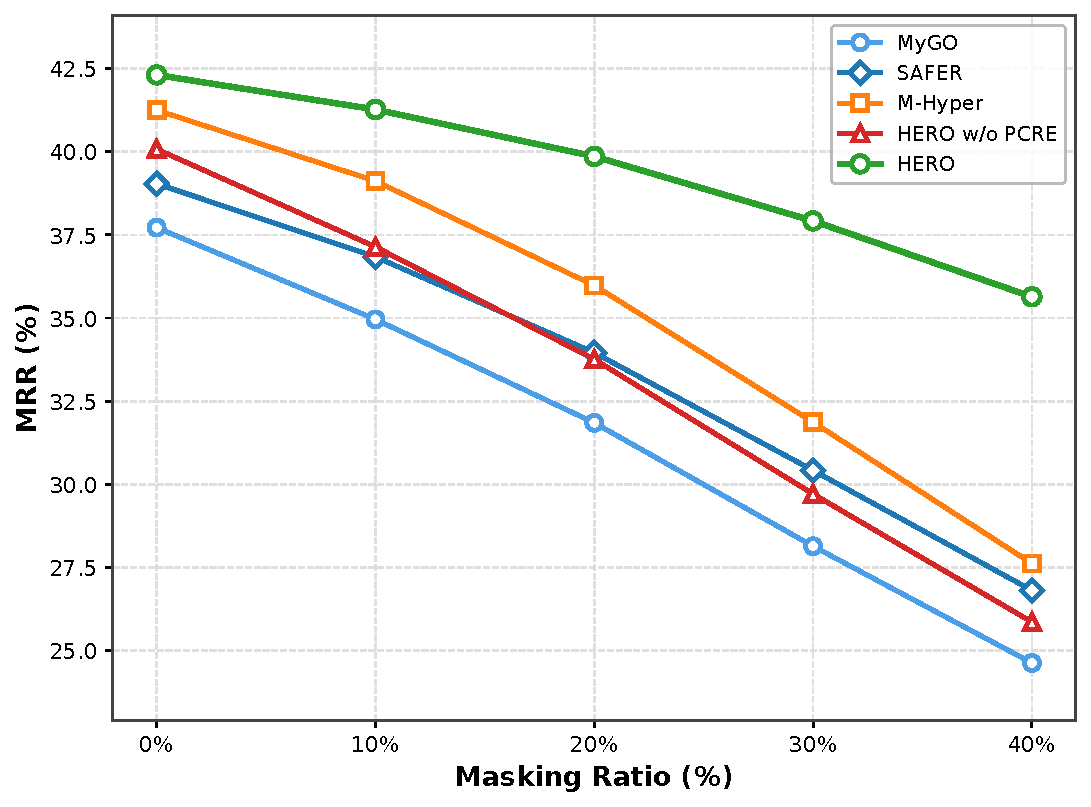
\includegraphics[width=0.3\textwidth]{DB15K_textual_noise.pdf}
    }
    \subfigure[Visual noise on DB15K]{
        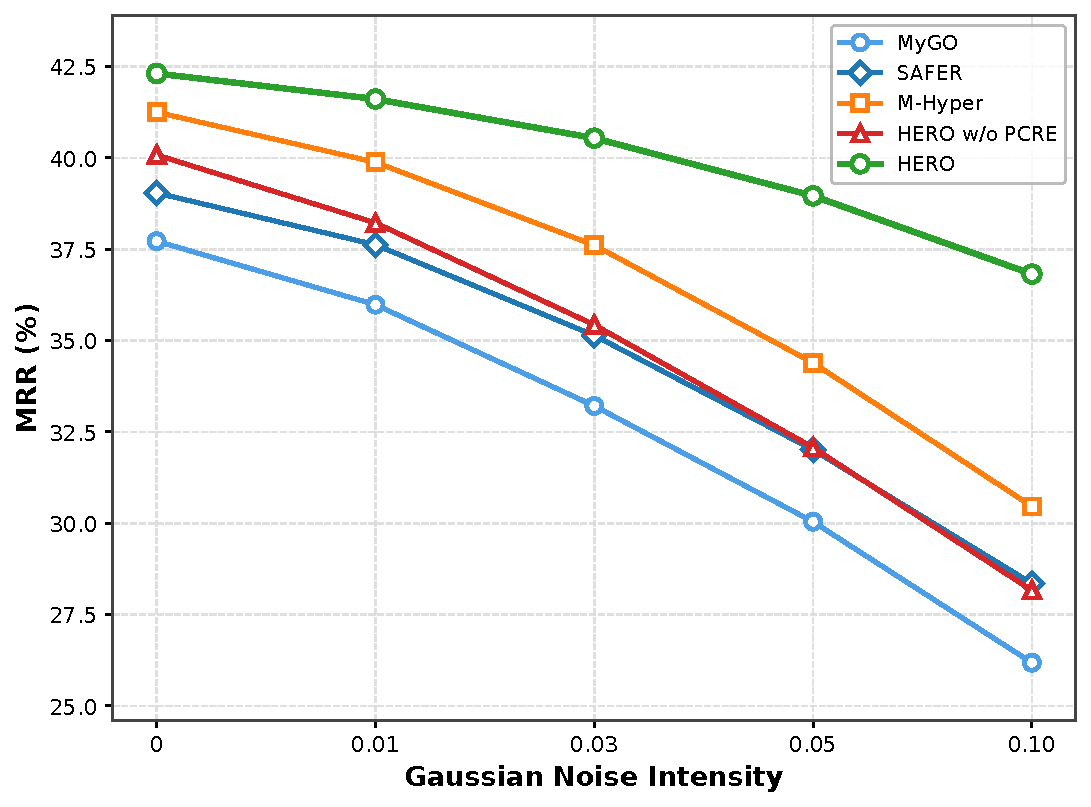
\includegraphics[width=0.3\textwidth]{DB15K_visual_noise.pdf}
    }
    \subfigure[Structural perturbation on DB15K]{
        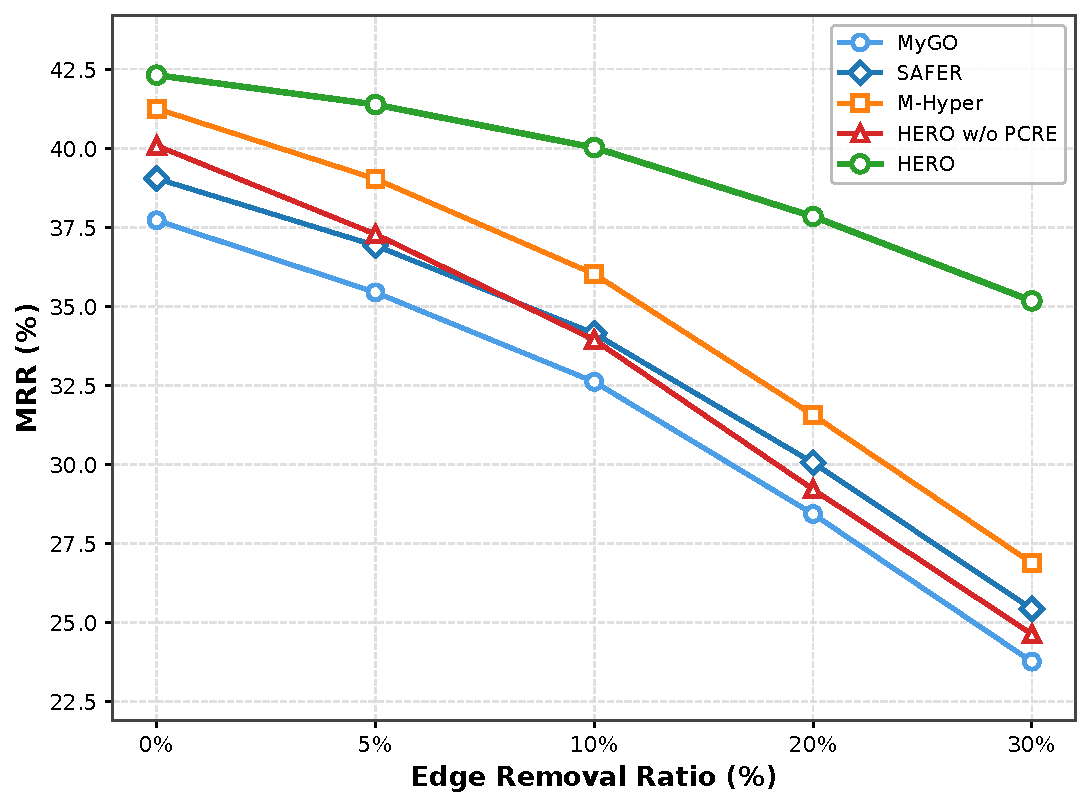
\includegraphics[width=0.3\textwidth]{DB15K_structural_perturbation.pdf}
    }
    \caption{Robustness analysis on DB15K under textual noise, visual noise, and structural perturbation. HERO maintains a slower performance degradation trend as the perturbation intensity increases, demonstrating stronger robustness under noisy multimodal and structural conditions.}
    \label{fig:robustness_db15k}
\end{figure*}

\begin{figure*}[t]
    \centering
    \subfigure[Textual noise on MKG-W]{
        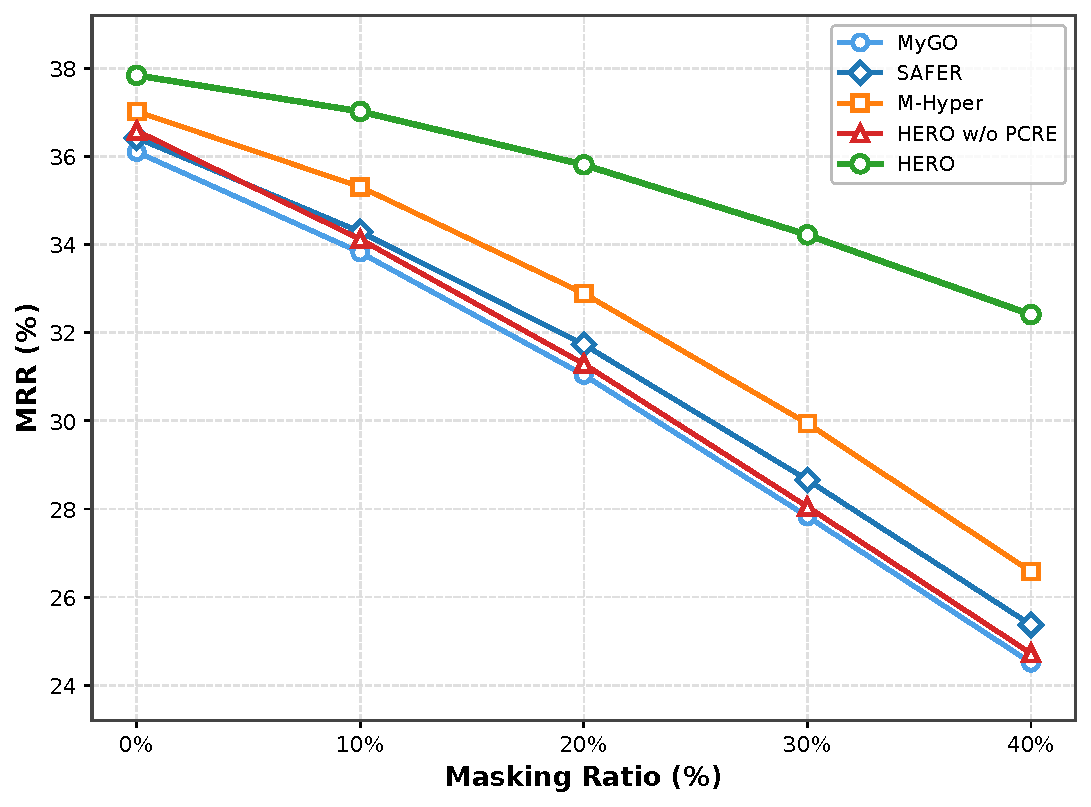
\includegraphics[width=0.3\textwidth]{MKG-W_textual_noise.pdf}
    }
    \subfigure[Visual noise on MKG-W]{
        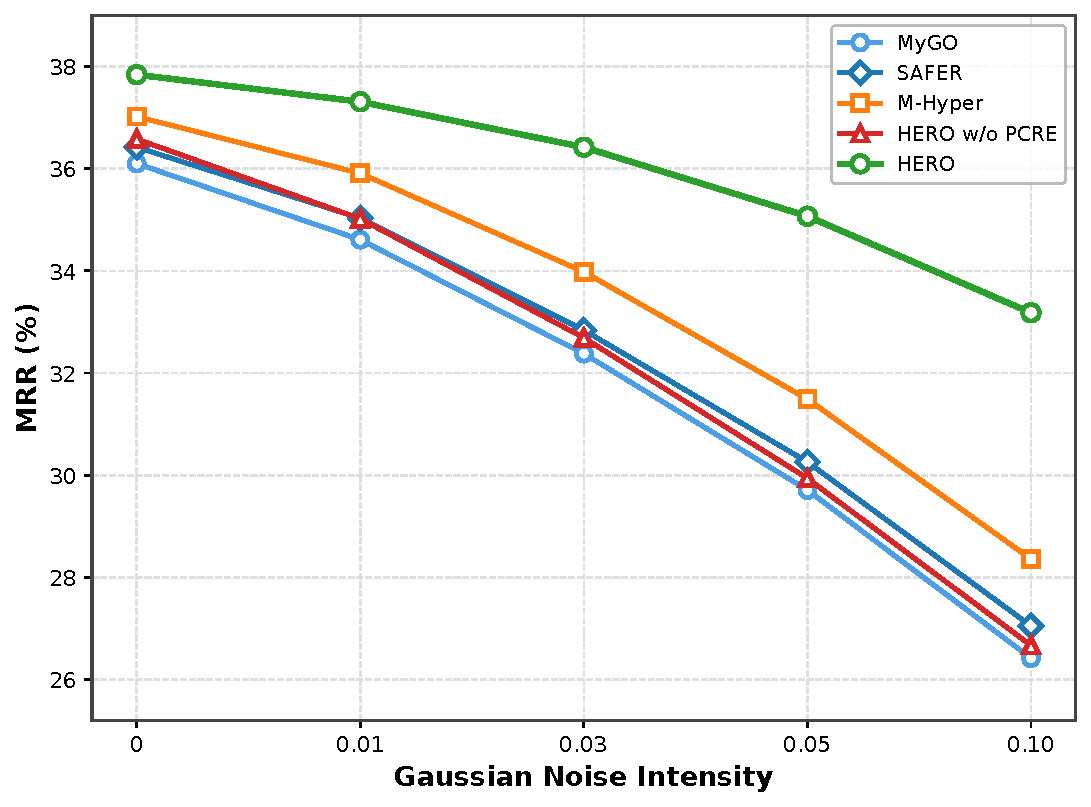
\includegraphics[width=0.3\textwidth]{MKG-W_visual_noise.pdf}
    }
    \subfigure[Structural perturbation on MKG-W]{
        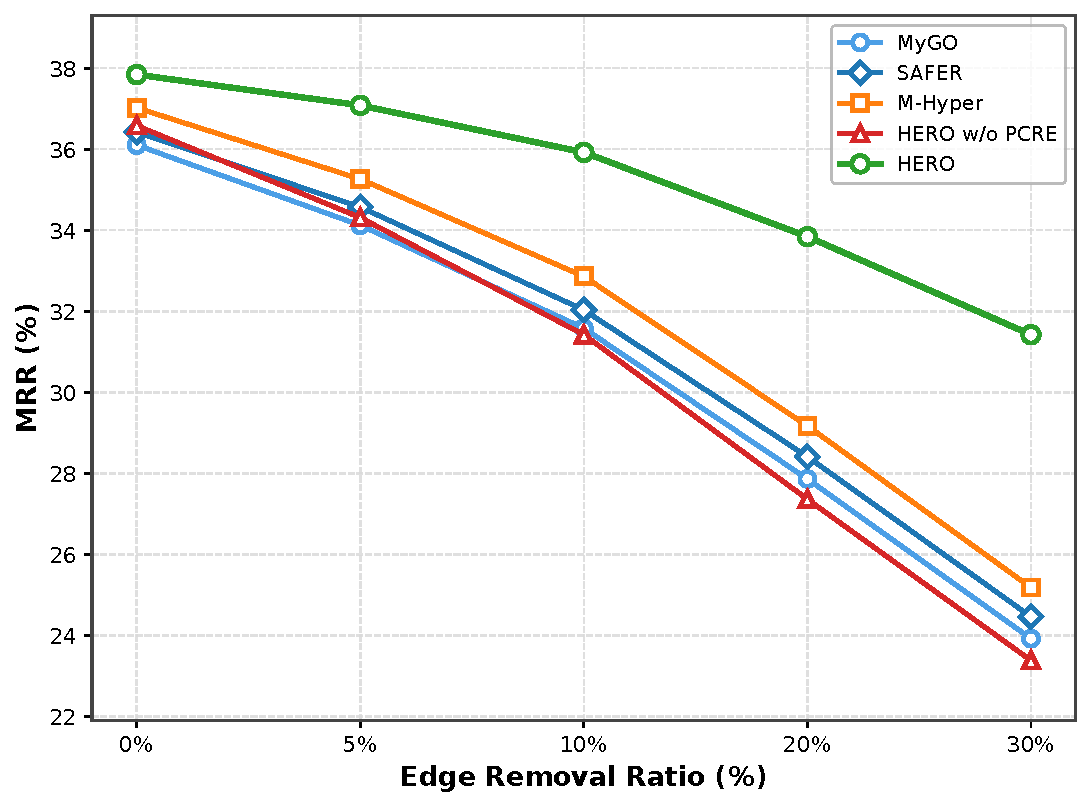
\includegraphics[width=0.3\textwidth]{MKG-W_structural_perturbation.pdf}
    }
    \caption{Robustness analysis on MKG-W under textual noise, visual noise, and structural perturbation. HERO consistently achieves higher MRR across different perturbation intensities, indicating that relation-aware local reasoning and perturbation consistency optimization help stabilize candidate fact prediction.}
    \label{fig:robustness_mkgw}
\end{figure*}

\begin{figure*}[t]
    \centering
    \subfigure[Textual noise on MKG-Y]{
        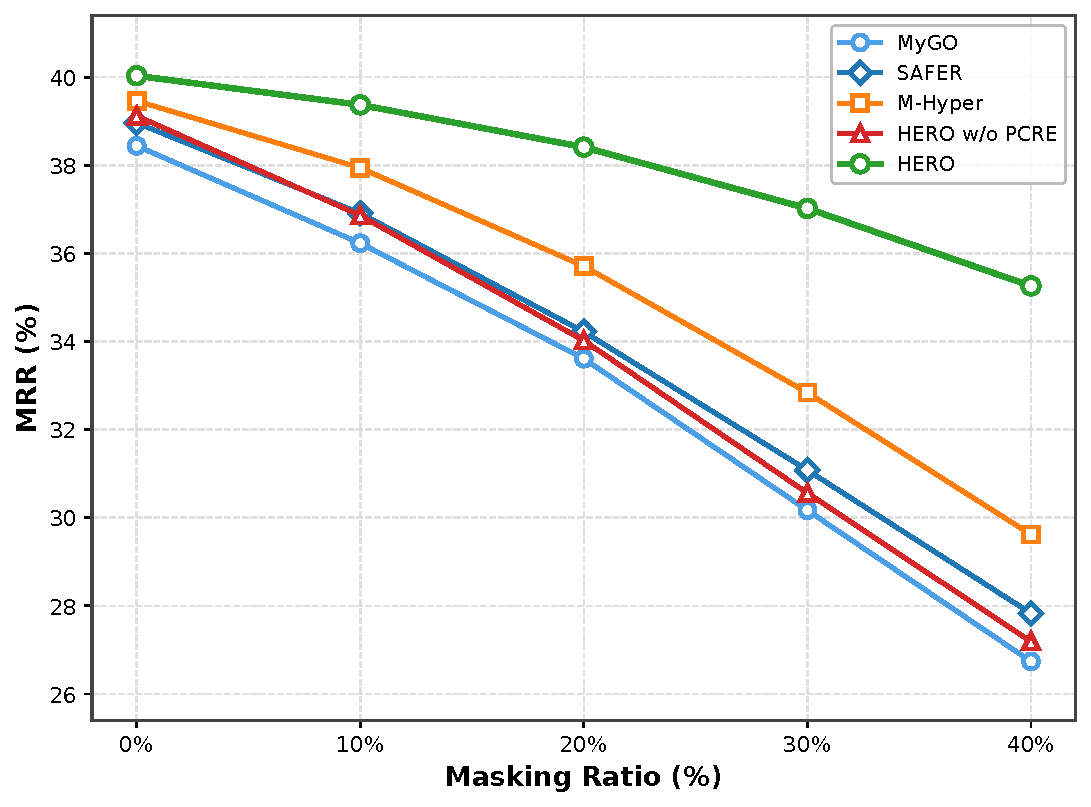
\includegraphics[width=0.3\textwidth]{MKG-Y_textual_noise.pdf}
    }
    \subfigure[Visual noise on MKG-Y]{
        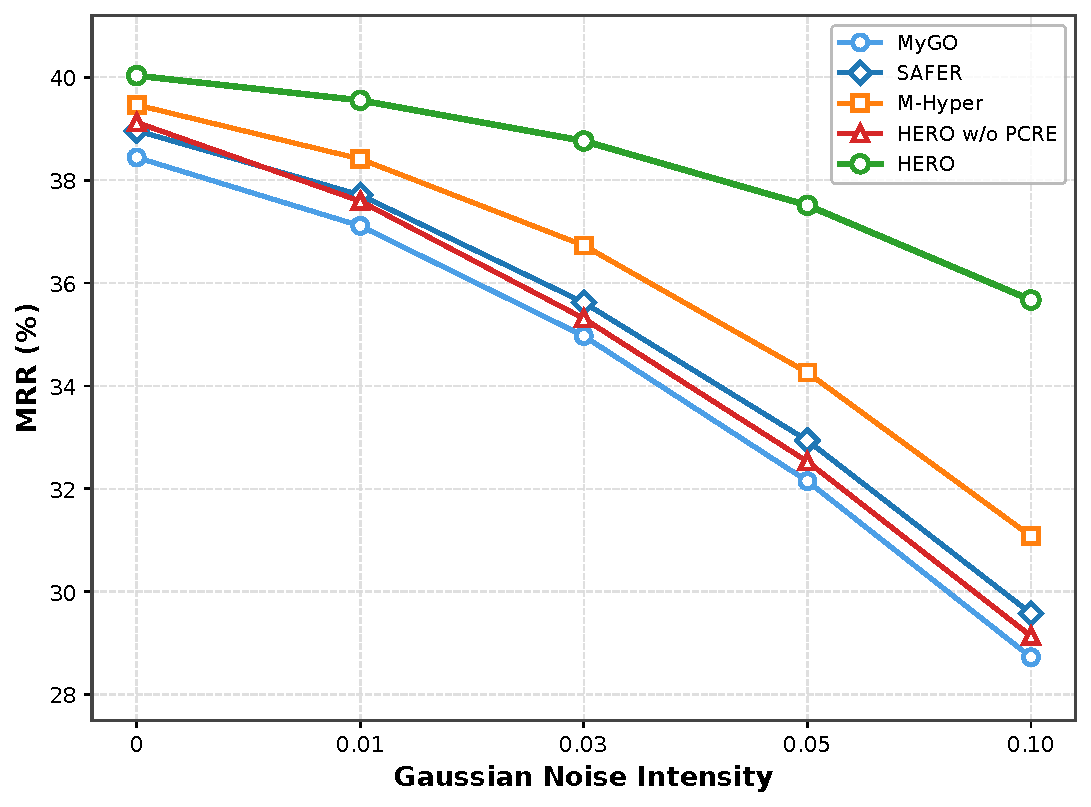
\includegraphics[width=0.3\textwidth]{MKG-Y_visual_noise.pdf}
    }
    \subfigure[Structural perturbation on MKG-Y]{
        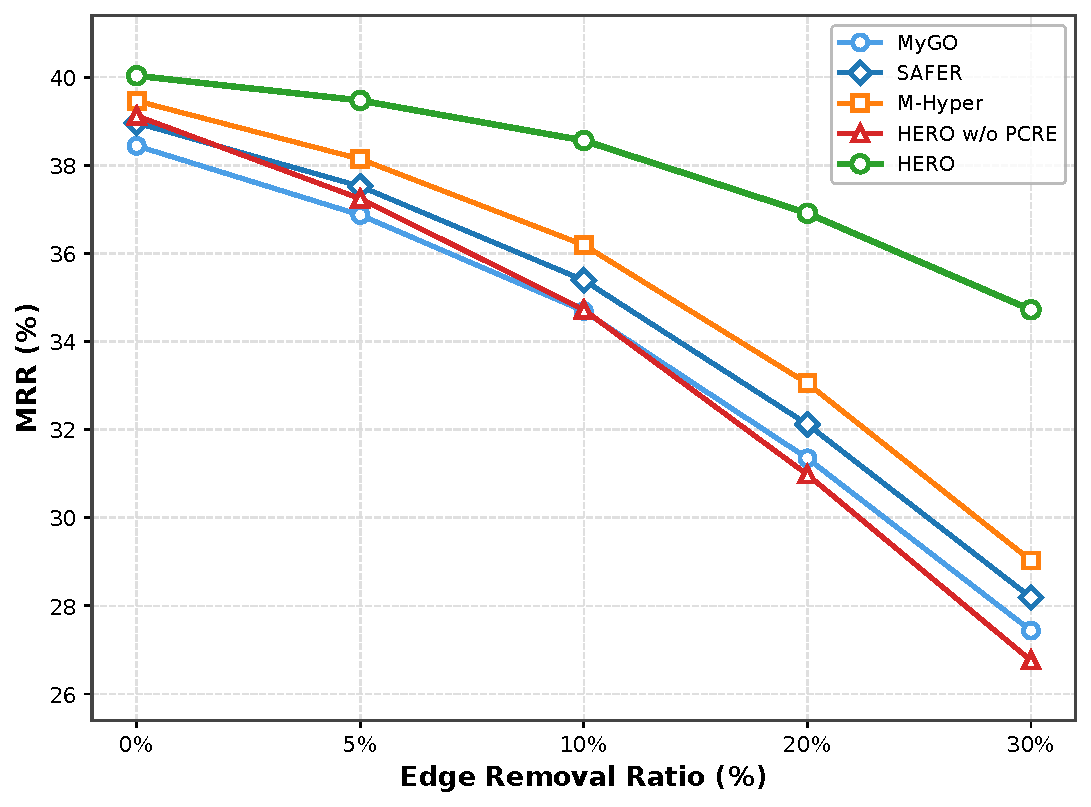
\includegraphics[width=0.3\textwidth]{MKG-Y_structural_perturbation.pdf}
    }
    \caption{Robustness analysis on MKG-Y under textual noise, visual noise, and structural perturbation. Compared with existing methods, HERO exhibits more stable performance under severe perturbations, demonstrating its ability to alleviate the influence of noisy modalities and incomplete structural connections.}
    \label{fig:robustness_mkgy}
\end{figure*}

As shown in Figures~\ref{fig:robustness_db15k}, \ref{fig:robustness_mkgw}, and \ref{fig:robustness_mkgy}, all methods degrade as textual, visual, or structural perturbations become stronger. Nevertheless, HERO consistently maintains flatter degradation curves and higher MRR across the three datasets. This indicates that its advantage is not limited to clean settings. Relation hypergraph modeling supplies high-order structural constraints, candidate-specific local reasoning introduces target-relevant evidence, and perturbation consistency prevents noisy modality or structural signals from being excessively amplified during propagation and scoring.



\begin{figure*}[t]
    \centering
    \subfigure[DB15K]{
        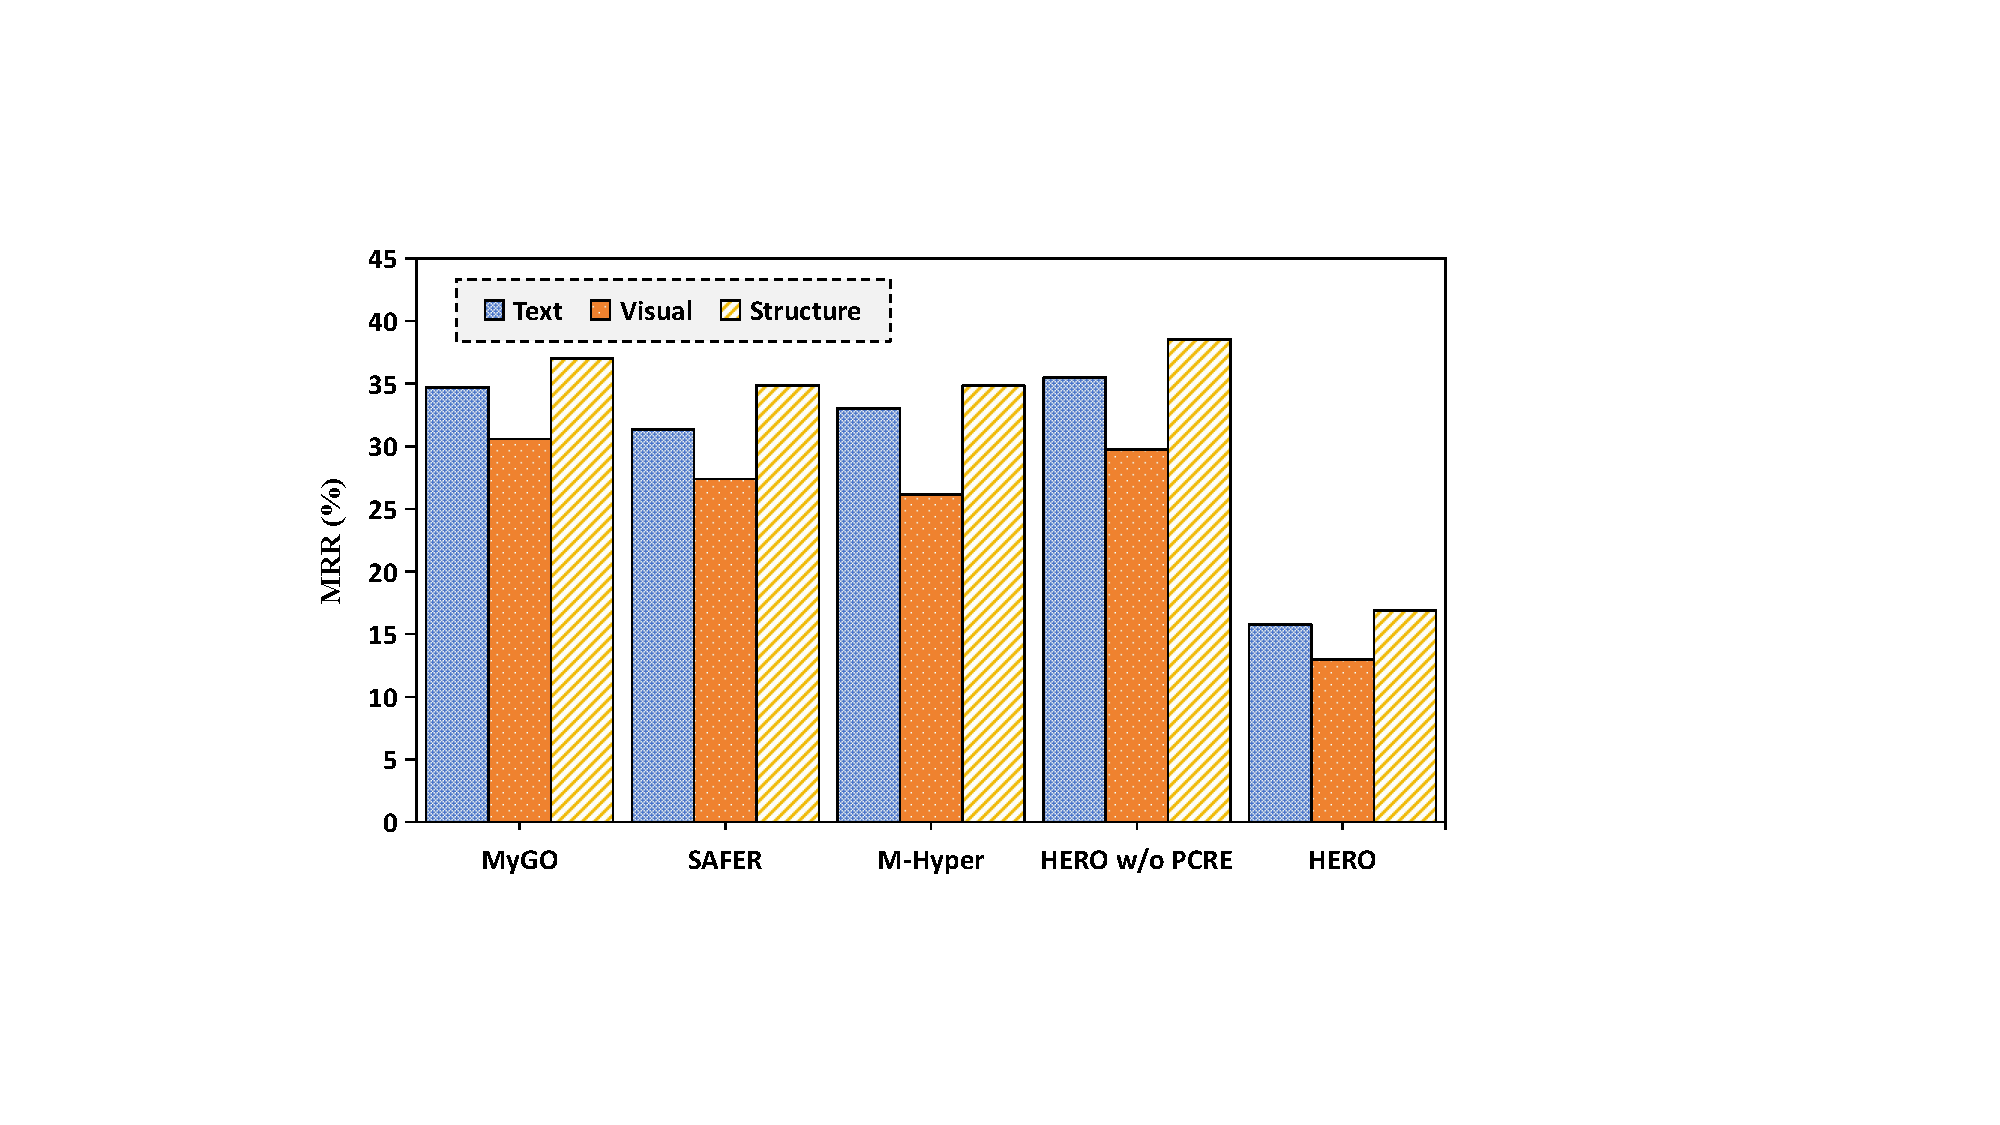
\includegraphics[width=0.3\textwidth]{barplot_DB15K_degradation.pdf}
    }
    \subfigure[MKG-W]{
        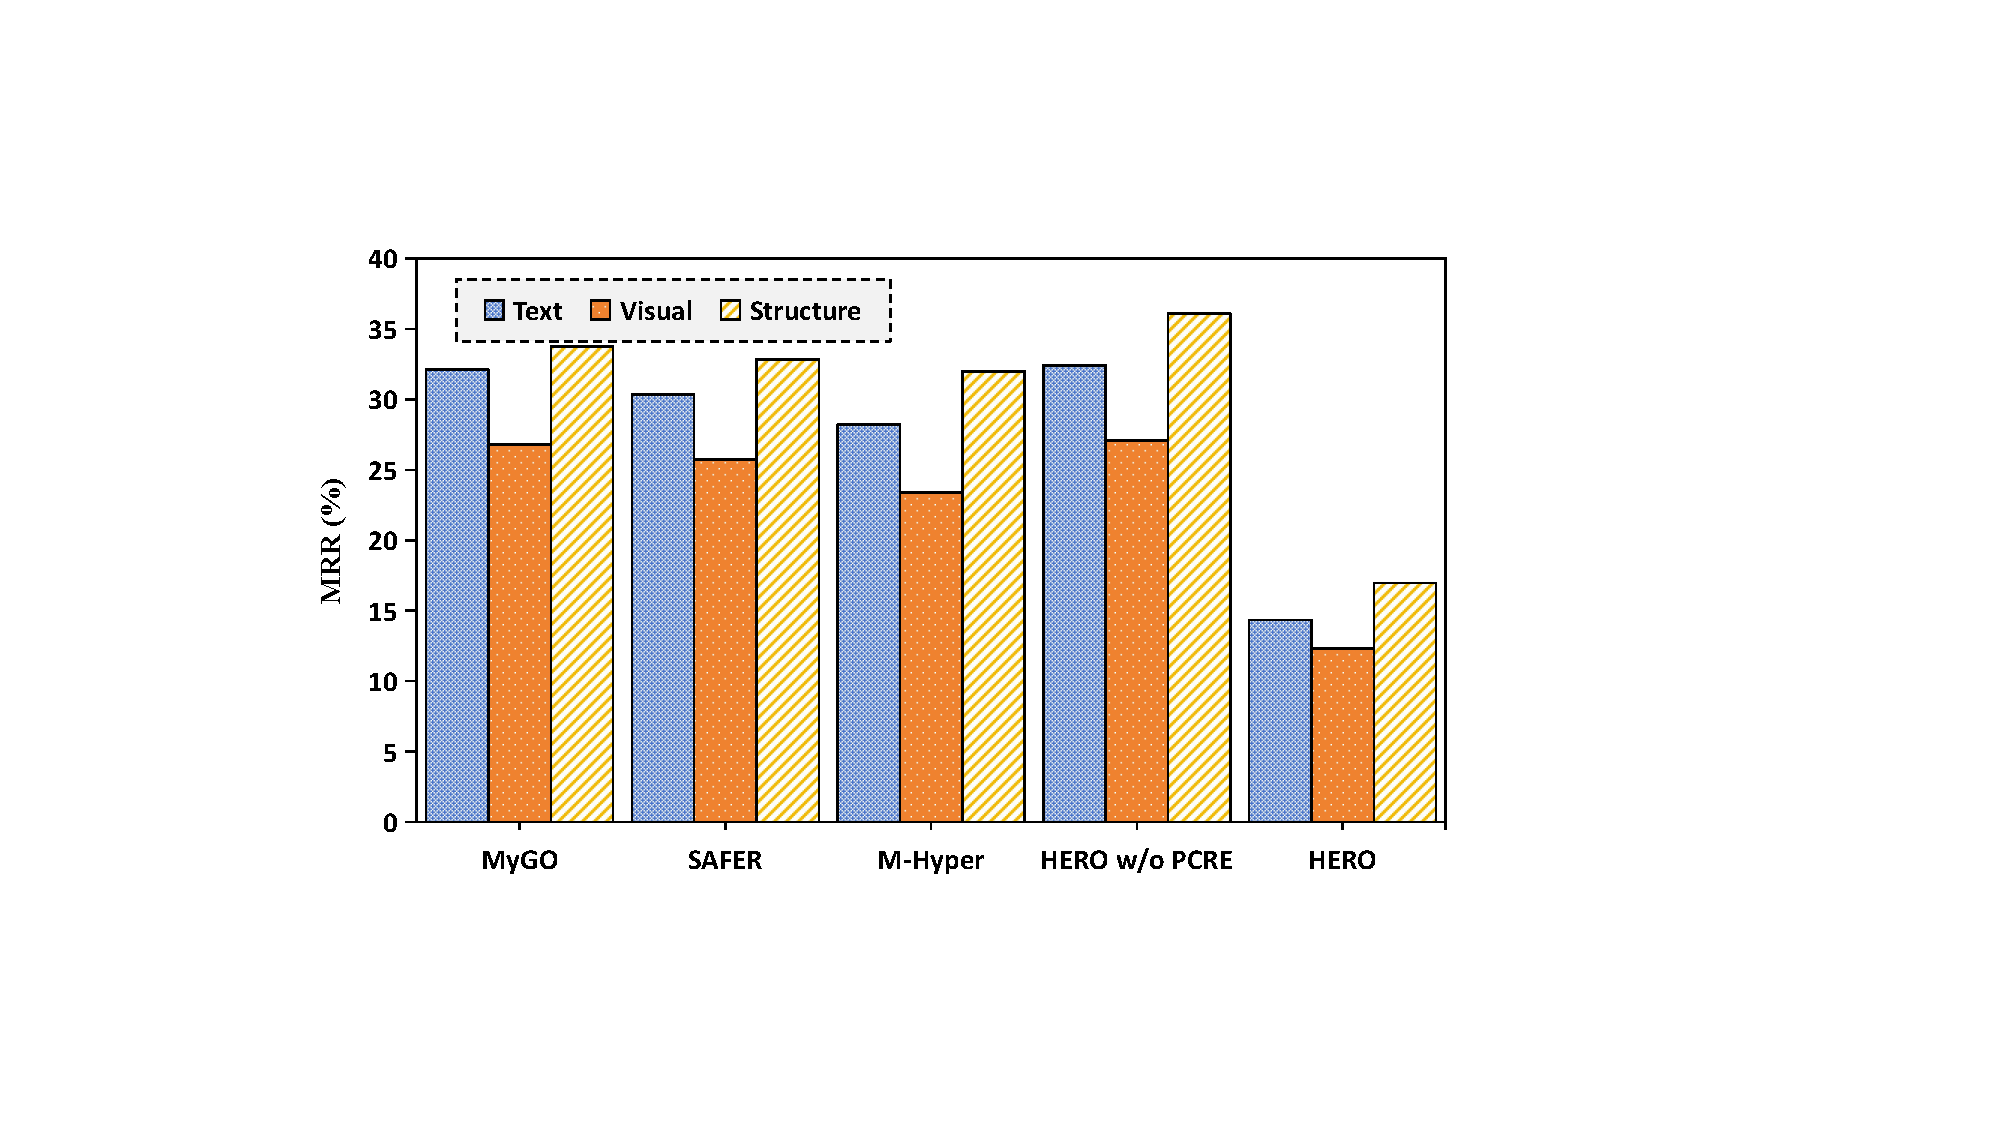
\includegraphics[width=0.3\textwidth]{barplot_MKG-W_degradation.pdf}
    }
    \subfigure[MKG-Y]{
        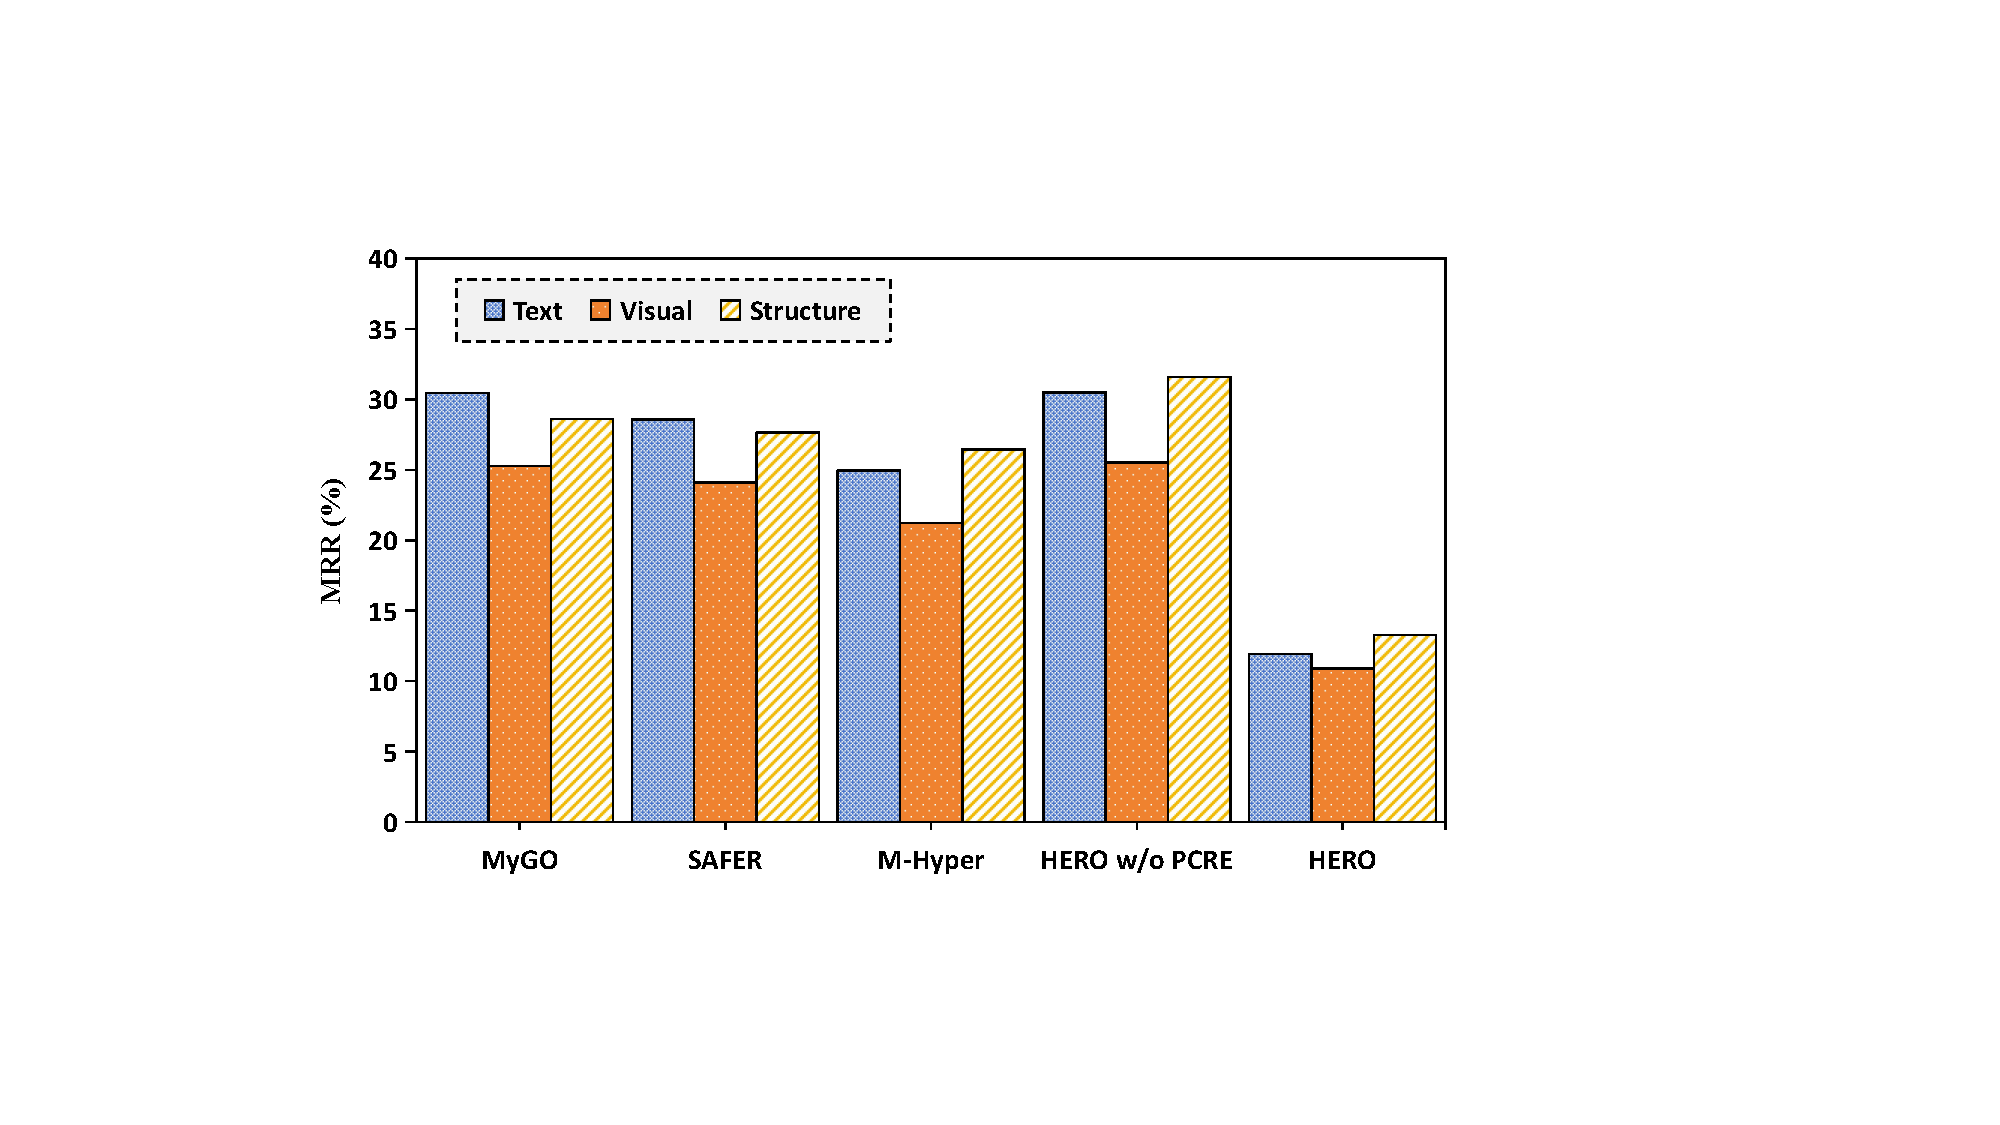
\includegraphics[width=0.3\textwidth]{barplot_MKG-Y_degradation.pdf}
    }
    \caption{Relative MRR degradation under the strongest textual, visual, and structural perturbations on three benchmark datasets. Lower degradation indicates stronger robustness. HERO consistently exhibits the smallest performance decline across different perturbation types and datasets, demonstrating its superior stability under noisy multimodal and structural conditions.}
    \label{fig:degradation_all}
\end{figure*}

Figure~\ref{fig:degradation_all} reports relative MRR degradation under the strongest perturbation level. HERO obtains the lowest degradation rates under all perturbation types, while HERO w/o PCRE declines more sharply. The gap highlights the importance of embedding- and score-level consistency when multimodal or structural information becomes unreliable.


\subsubsection{Effectiveness of Relation Hypergraph-based High-order Modeling}

Relation hypergraph modeling is analyzed from three perspectives. First, HERO is compared with structural variants to examine whether hypergraph convolution is more expressive than pairwise modeling. Second, test triples are divided by relation frequency to assess sparse-relation behavior. Third, relations are grouped by hyperedge size to study whether larger relation-specific entity groups strengthen the advantage of HERO. The results are shown in Figure~\ref{fig:hypergraph_analysis}.

\begin{figure*}[t]
    \centering
    \subfigure[Structural variant comparison]{
        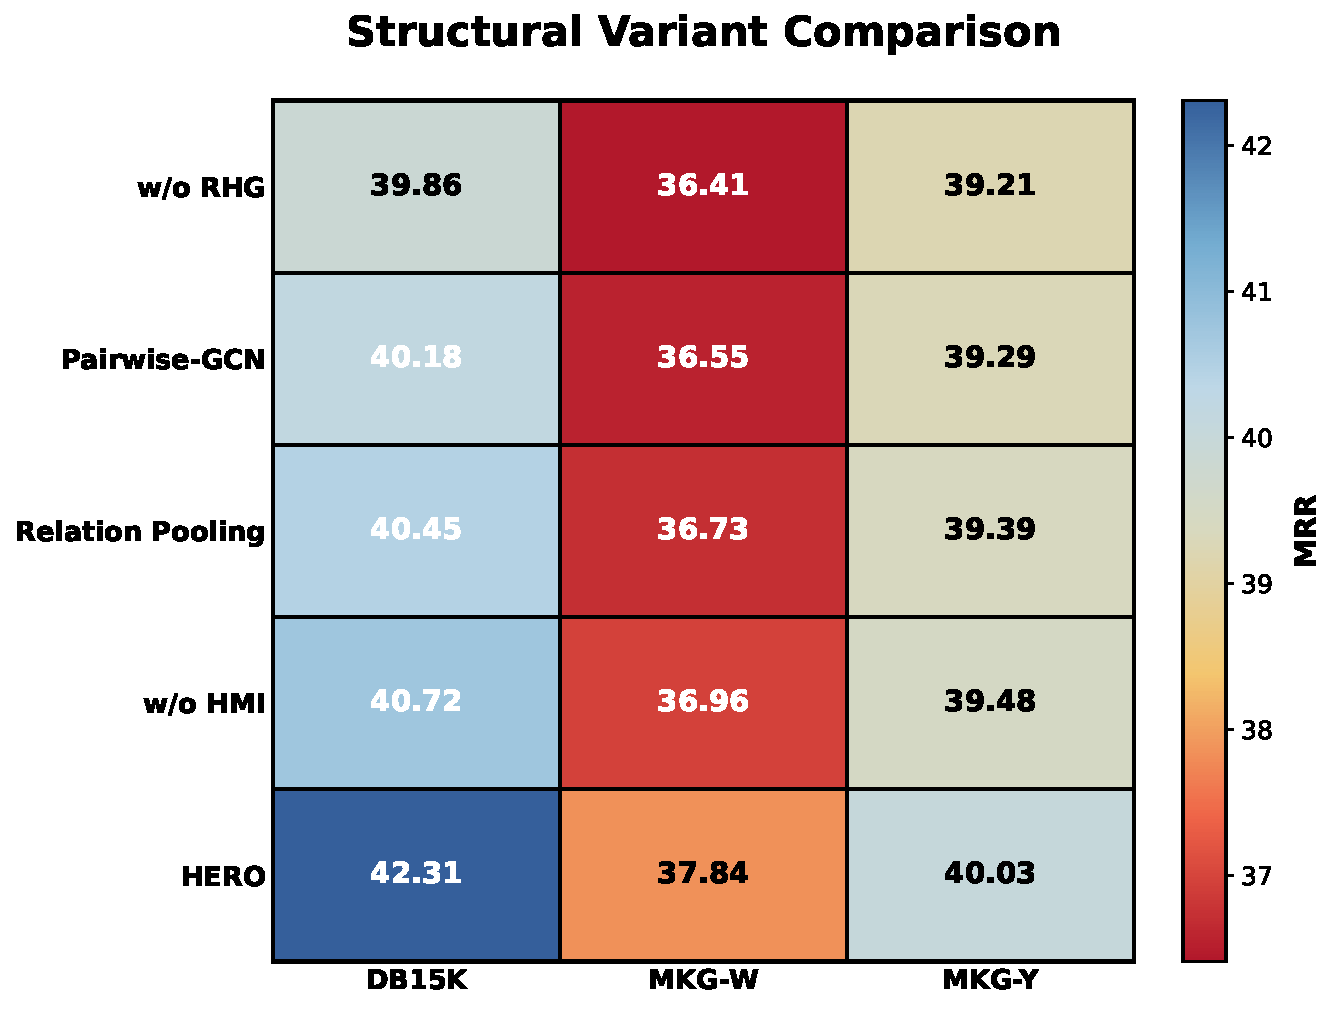
\includegraphics[width=0.3\textwidth]{hypergraph_variant_heatmap2.pdf}
    }
    \subfigure[Relation-frequency groups]{
        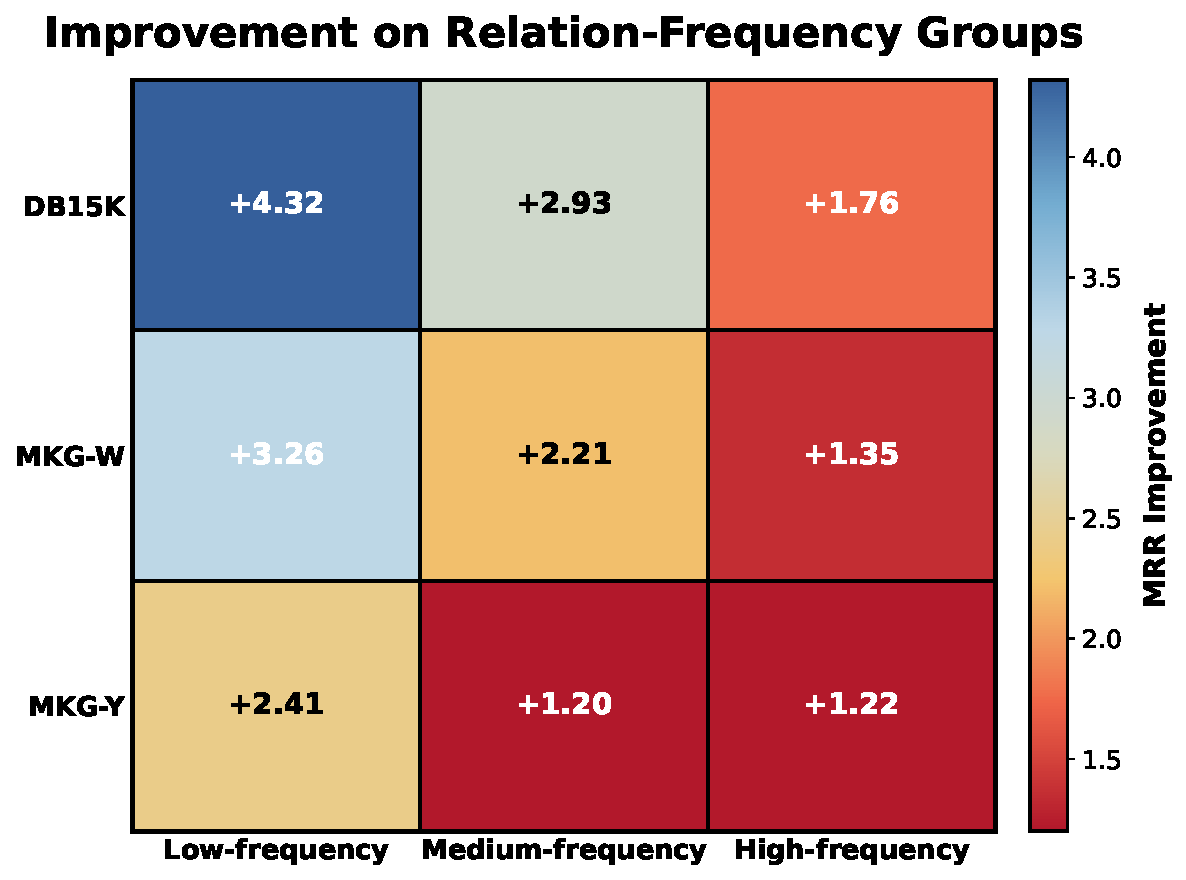
\includegraphics[width=0.3\textwidth]{relation_frequency_heatmap2.pdf}
    }
    \subfigure[Hyperedge-size groups]{
        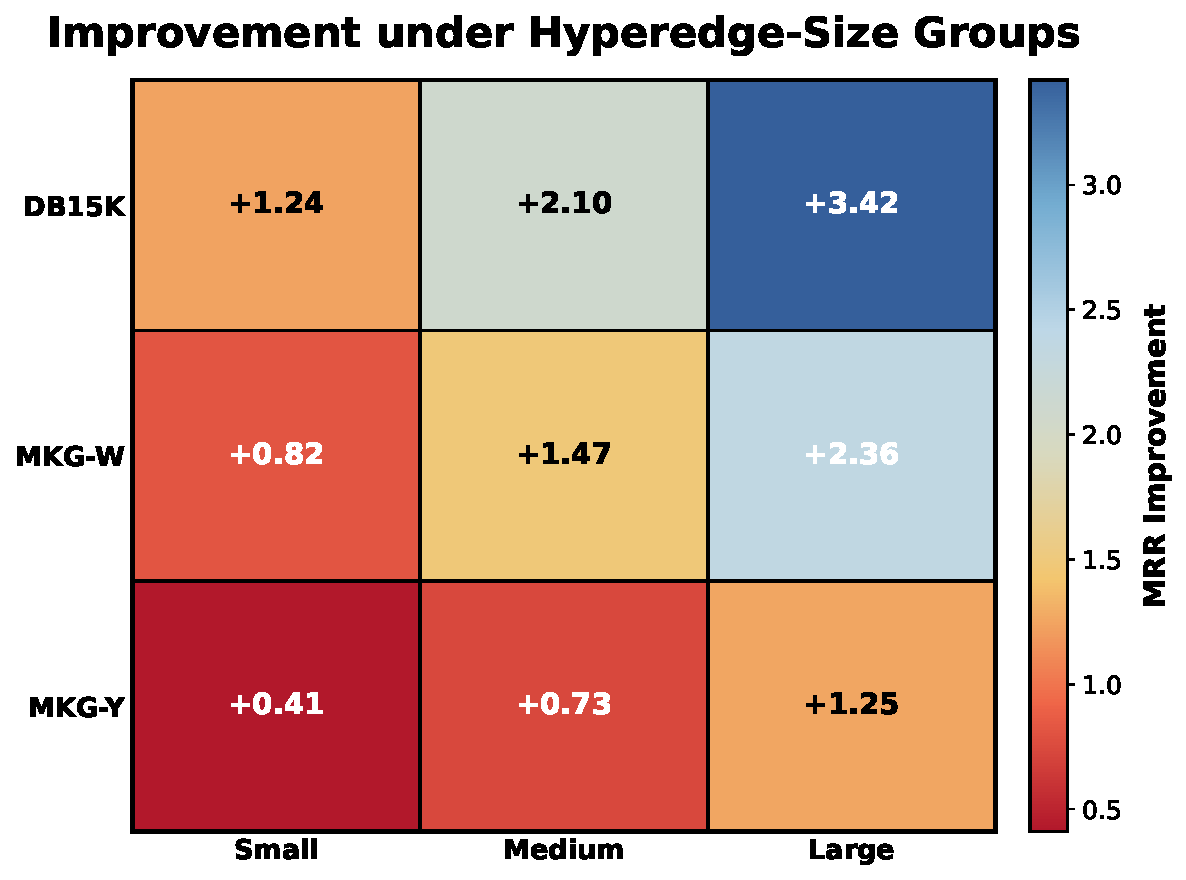
\includegraphics[width=0.3\textwidth]{hyperedge_size_heatmap2.pdf}
    }
    \caption{Effectiveness analysis of relation hypergraph modeling. 
    (a) MRR comparison among different structural variants on three datasets. 
    (b) MRR improvement of HERO over Pairwise-GCN on different relation-frequency groups. 
    (c) MRR improvement of HERO over Pairwise-GCN under different hyperedge-size groups. 
    Darker colors indicate higher MRR or larger improvement.}
    \label{fig:hypergraph_analysis}
\end{figure*}

Figure~\ref{fig:hypergraph_analysis}(a) compares HERO with structural variants, including \textbf{w/o RHG}, \textbf{Pairwise-GCN}, \textbf{Relation Pooling}, and \textbf{w/o HMI}. HERO consistently achieves the highest MRR, indicating that relation-specific hyperedges are more expressive than pairwise propagation or simple relation-level pooling. Compared with \textbf{w/o RHG}, HERO improves MRR by 2.45, 1.43, and 0.82 percentage points on DB15K, MKG-W, and MKG-Y, respectively, with the largest gain on the relation-rich DB15K dataset.

Figures~\ref{fig:hypergraph_analysis}(b) and (c) further show larger gains over Pairwise-GCN for low-frequency relations and larger hyperedges. Relation hypergraphs therefore help sparse relations by sharing information among entities with the same relation semantics, and their benefit becomes clearer when a relation connects many entities.


\subsubsection{Effectiveness of Candidate-specific Context-aware Reasoning}

Candidate-specific reasoning is evaluated with variants that use different local contexts. \textbf{Global Scoring} uses only pre-trained entity and relation embeddings. \textbf{Neighborhood-only} and \textbf{Path-only} use dual-end neighborhoods and connecting multi-hop paths, respectively. \textbf{Random Paths} replaces relation-relevant paths with random paths under the same length constraint, while \textbf{Full Subgraph} combines neighborhoods and relation-relevant paths without the complete perturbation-consistent optimization strategy. The full HERO model additionally uses relation-aware graph attention and perturbation consistency. The results are presented in Figure~\ref{fig:local_reasoning}.

\begin{figure*}[t]
    \centering
    \subfigure[MRR comparison on DB15K]{
        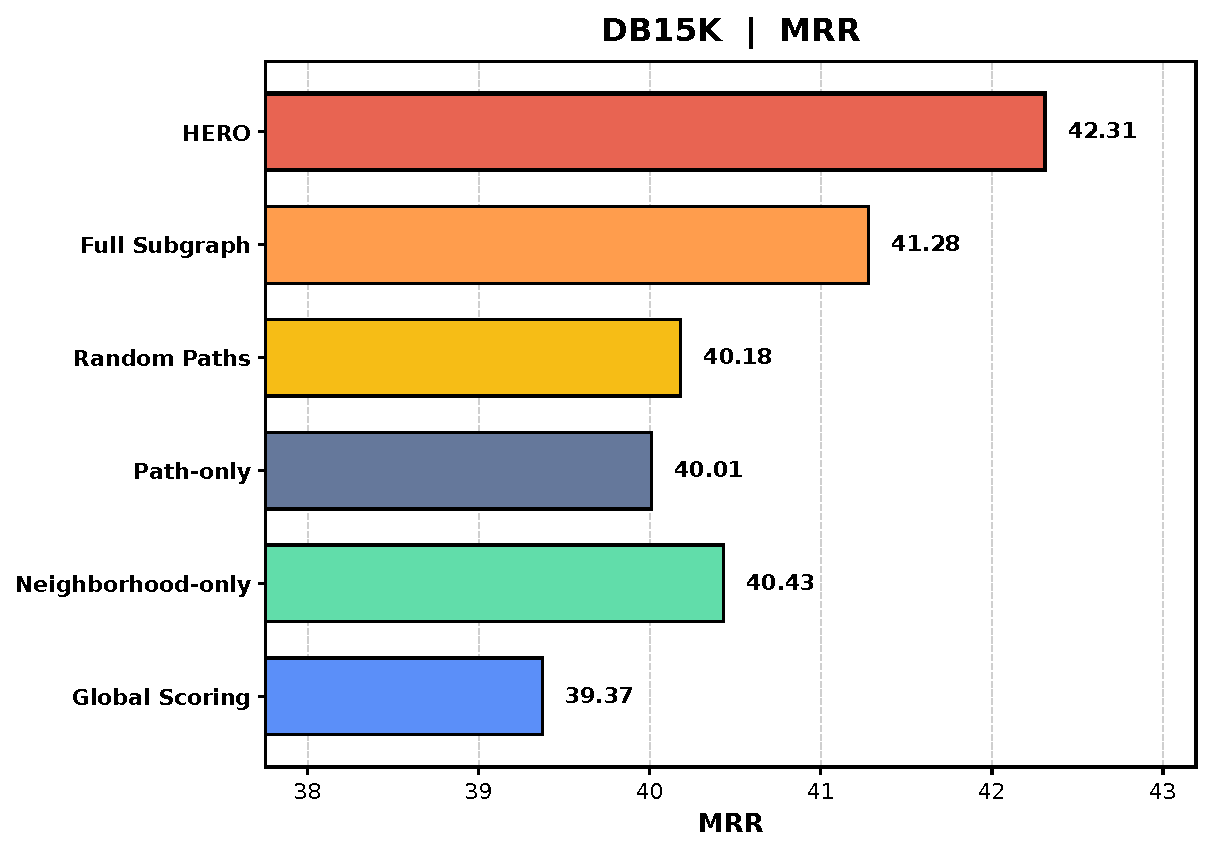
\includegraphics[width=0.3\textwidth]{DB15K_MRR_horizontal_bar.pdf}
    }
    \subfigure[Hits@10 comparison on DB15K]{
        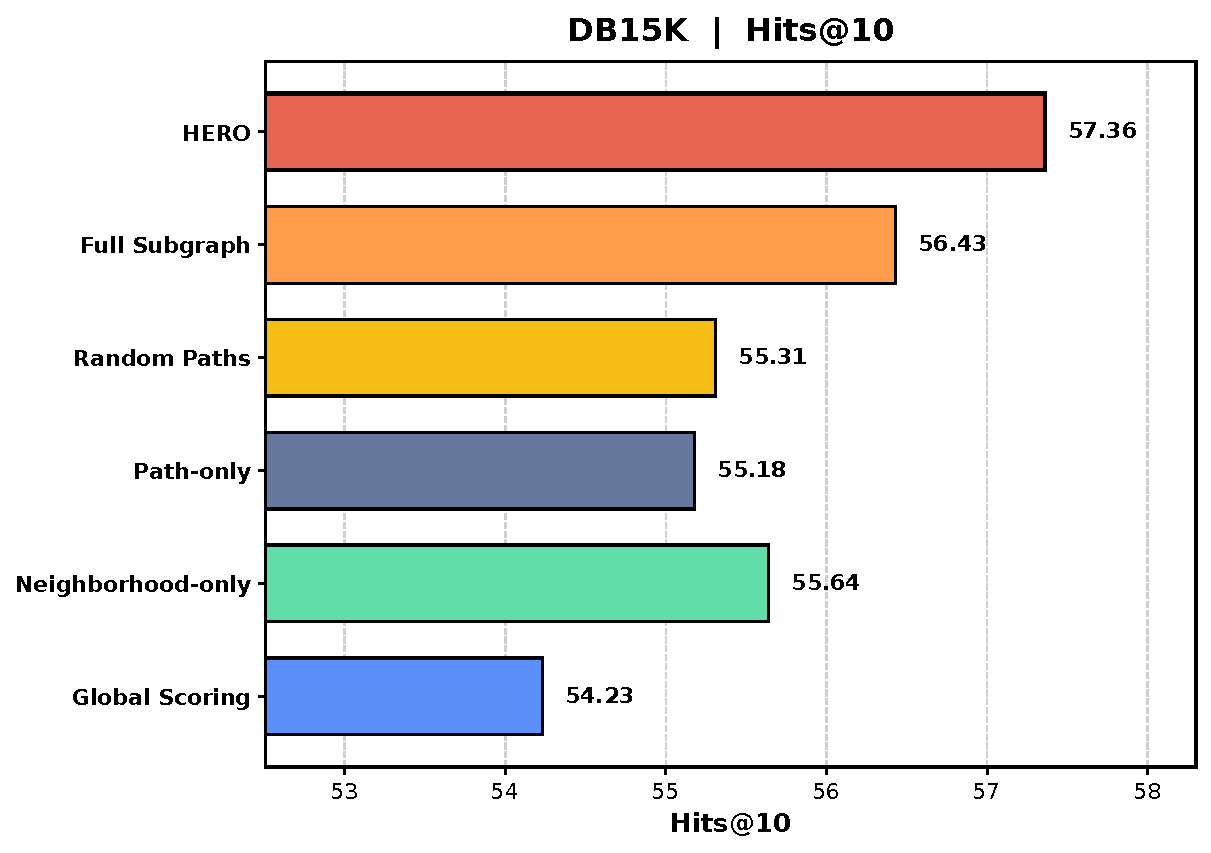
\includegraphics[width=0.3\textwidth]{DB15K_Hitsat10_horizontal_bar.pdf}
    }
    \subfigure[MRR comparison on MKG-W]{
        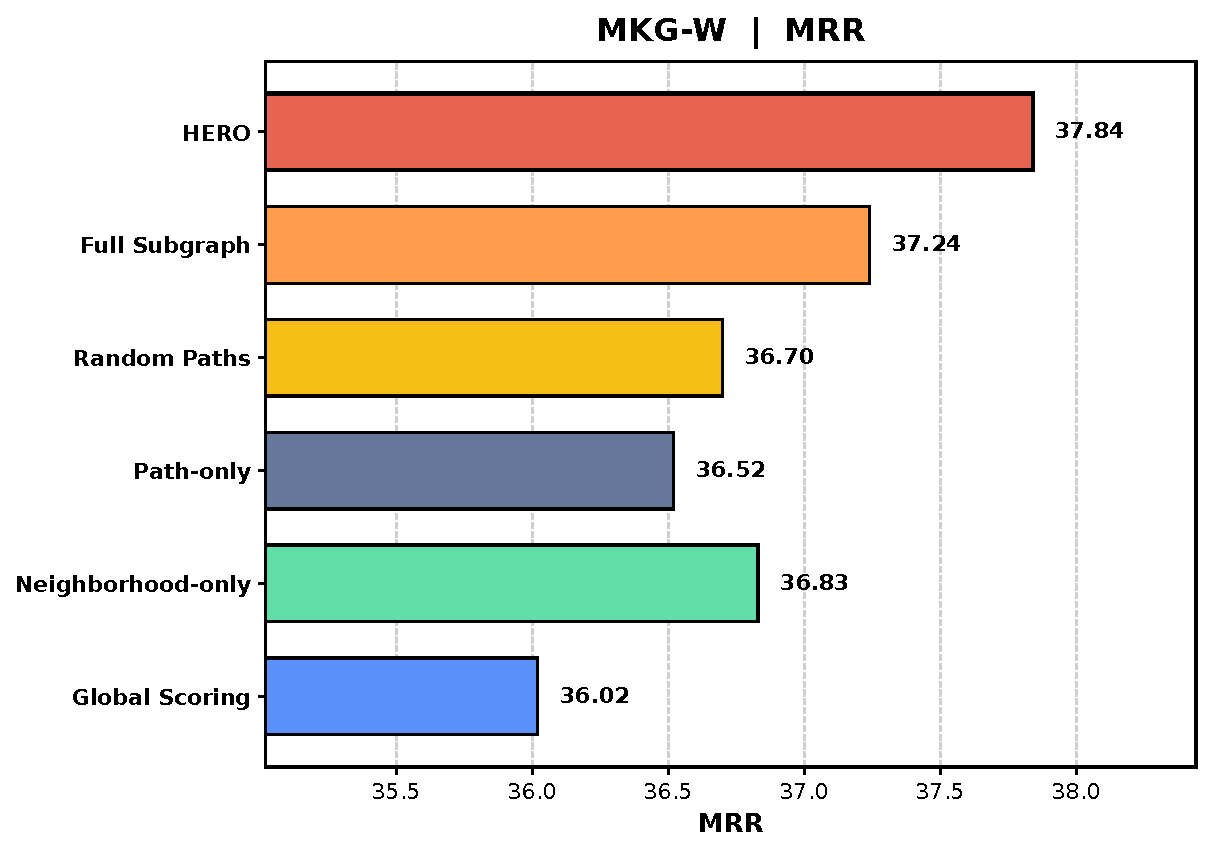
\includegraphics[width=0.3\textwidth]{MKG-W_MRR_horizontal_bar.pdf}
    }
    \subfigure[Hits@10 comparison on MKG-W]{
        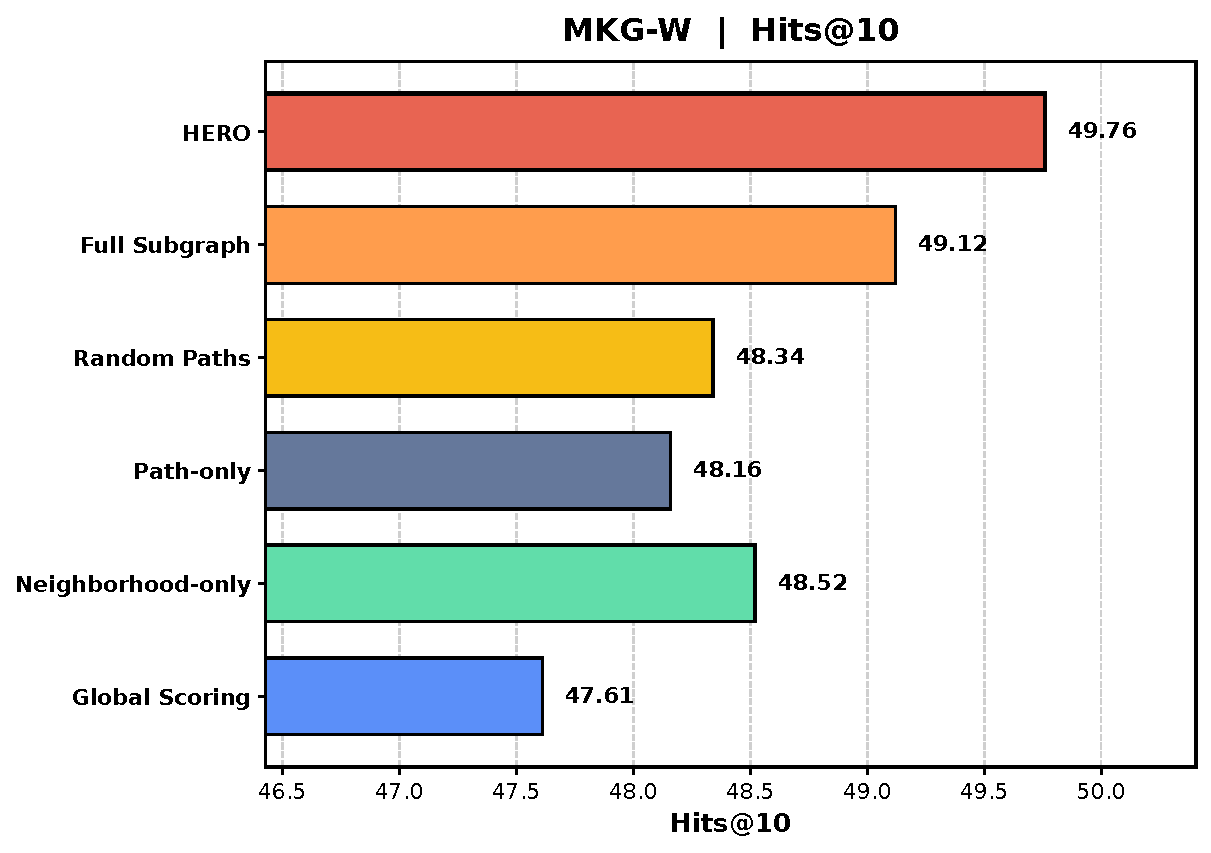
\includegraphics[width=0.3\textwidth]{MKG-W_Hitsat10_horizontal_bar.pdf}
    }
    \subfigure[MRR comparison on MKG-Y]{
        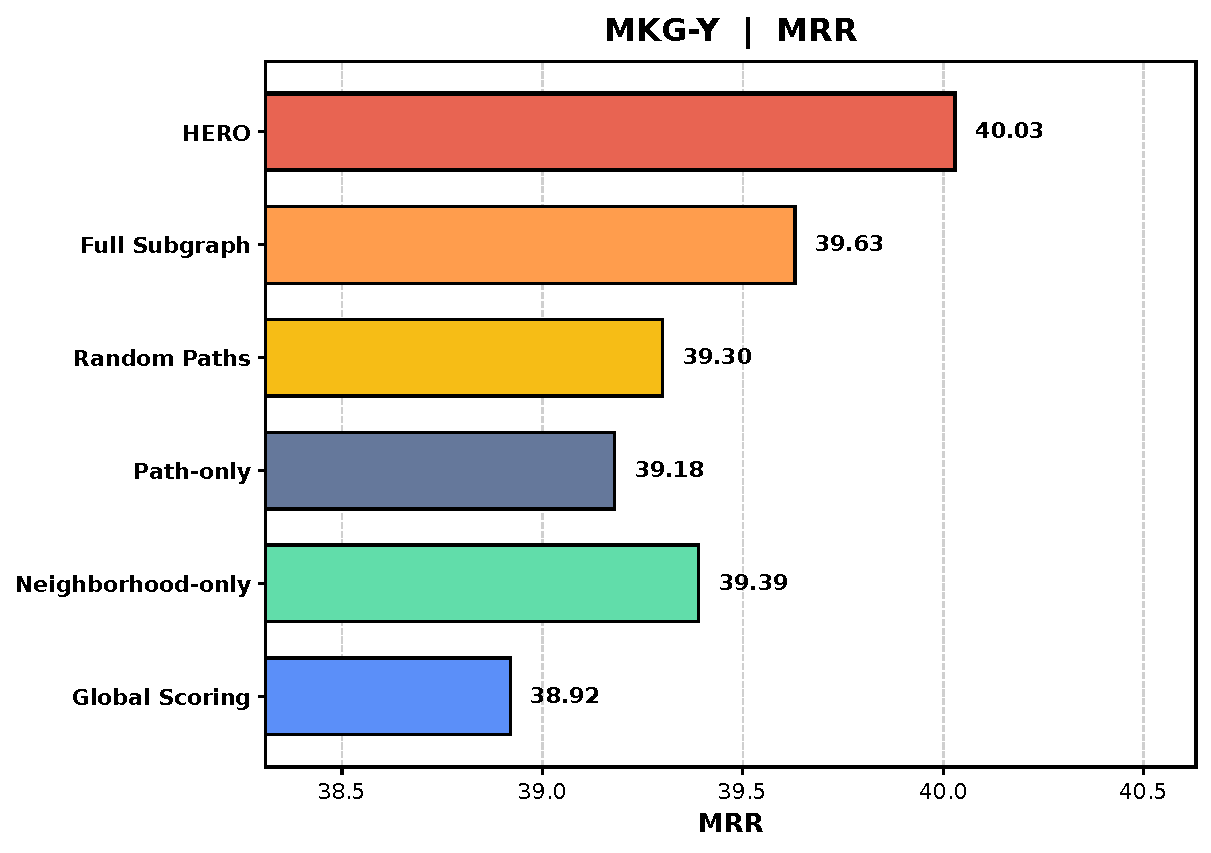
\includegraphics[width=0.3\textwidth]{MKG-Y_MRR_horizontal_bar.pdf}
    }
    \subfigure[Hits@10 comparison on MKG-Y]{
        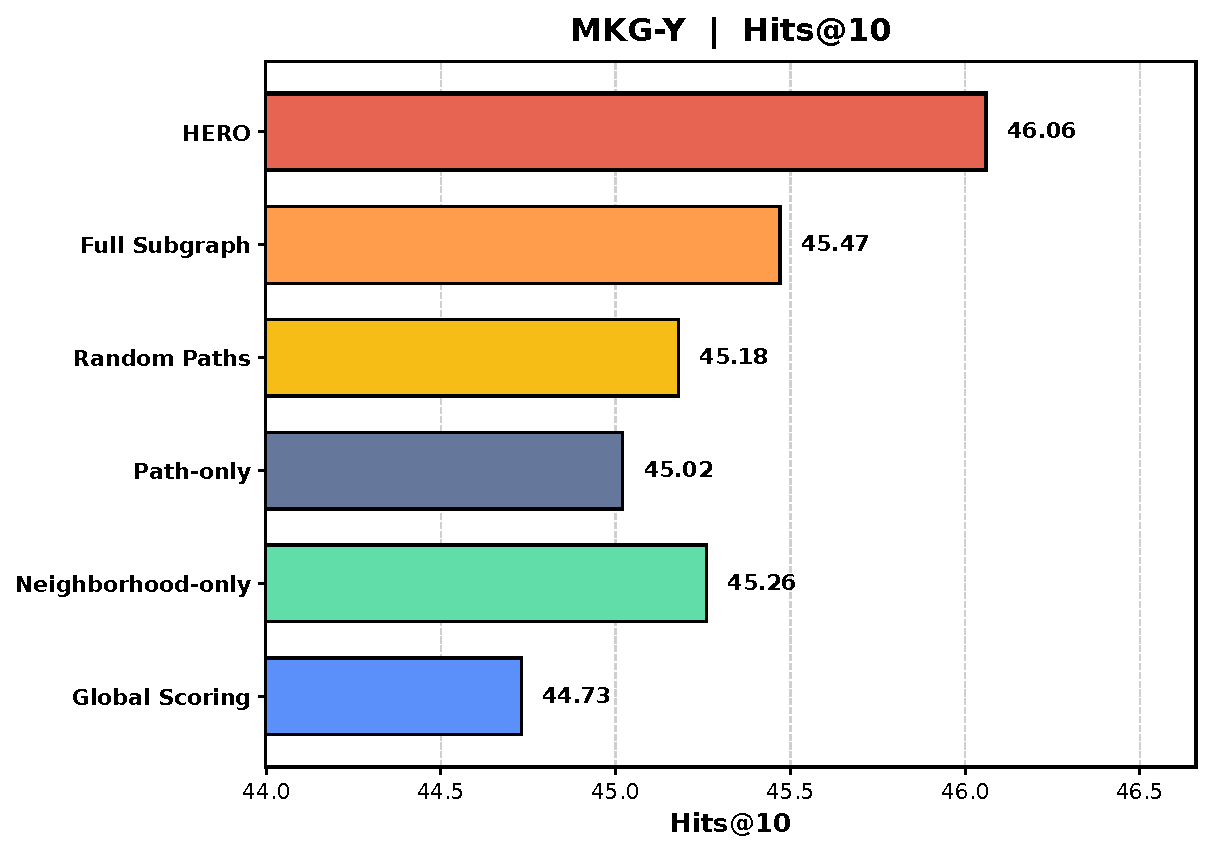
\includegraphics[width=0.3\textwidth]{MKG-Y_Hitsat10_horizontal_bar.pdf}
    }
    \caption{Effectiveness analysis of candidate-specific context-aware reasoning. 
    The six horizontal bar charts report MRR and Hits@10 of different local reasoning variants on DB15K, MKG-W, and MKG-Y. 
    The consistent advantage of HERO demonstrates that dual-end neighborhoods, relation-relevant multi-hop paths, relation-aware propagation, and perturbation-consistent optimization jointly improve candidate-specific structural reasoning.}
    \label{fig:local_reasoning}
\end{figure*}

As shown in Figure~\ref{fig:local_reasoning}, HERO consistently achieves the best MRR and Hits@10. Compared with \textbf{Global Scoring}, it improves MRR by 2.94, 1.82, and 1.11 percentage points on DB15K, MKG-W, and MKG-Y, respectively, showing that global pre-trained embeddings alone are insufficient for candidate fact prediction.

The variants clarify the role of local evidence. \textbf{Neighborhood-only} and \textbf{Path-only} both improve over global scoring, while \textbf{Full Subgraph} performs better by combining the two. The gap between \textbf{Random Paths} and \textbf{Full Subgraph} shows that path relevance matters. The complete HERO model further benefits from relation-aware graph attention and perturbation consistency, which integrate local evidence under target-relation guidance and stabilize the scores.



\subsubsection{Parameter Sensitivity Analysis}

Parameter sensitivity is analyzed on DB15K, MKG-W, and MKG-Y for six hyperparameters: embedding dimension $d$, hypergraph convolution depth $L$, neighborhood hop size $K$, number of selected relation-relevant paths $K_p$, perturbation strength $\sigma$, and consistency weight $\lambda_c$. Here, $\sigma$ is shared by entity and relation perturbations, and $\lambda_c$ is shared by embedding- and score-level consistency losses. One hyperparameter is varied at a time, with the others fixed to their validation-selected values. MRR is used as the metric, and the results are shown in Figure~\ref{fig:parameter_sensitivity}.

\begin{figure*}[t]
    \centering
    \subfigure[Sensitivity to representation dimensionality]{
        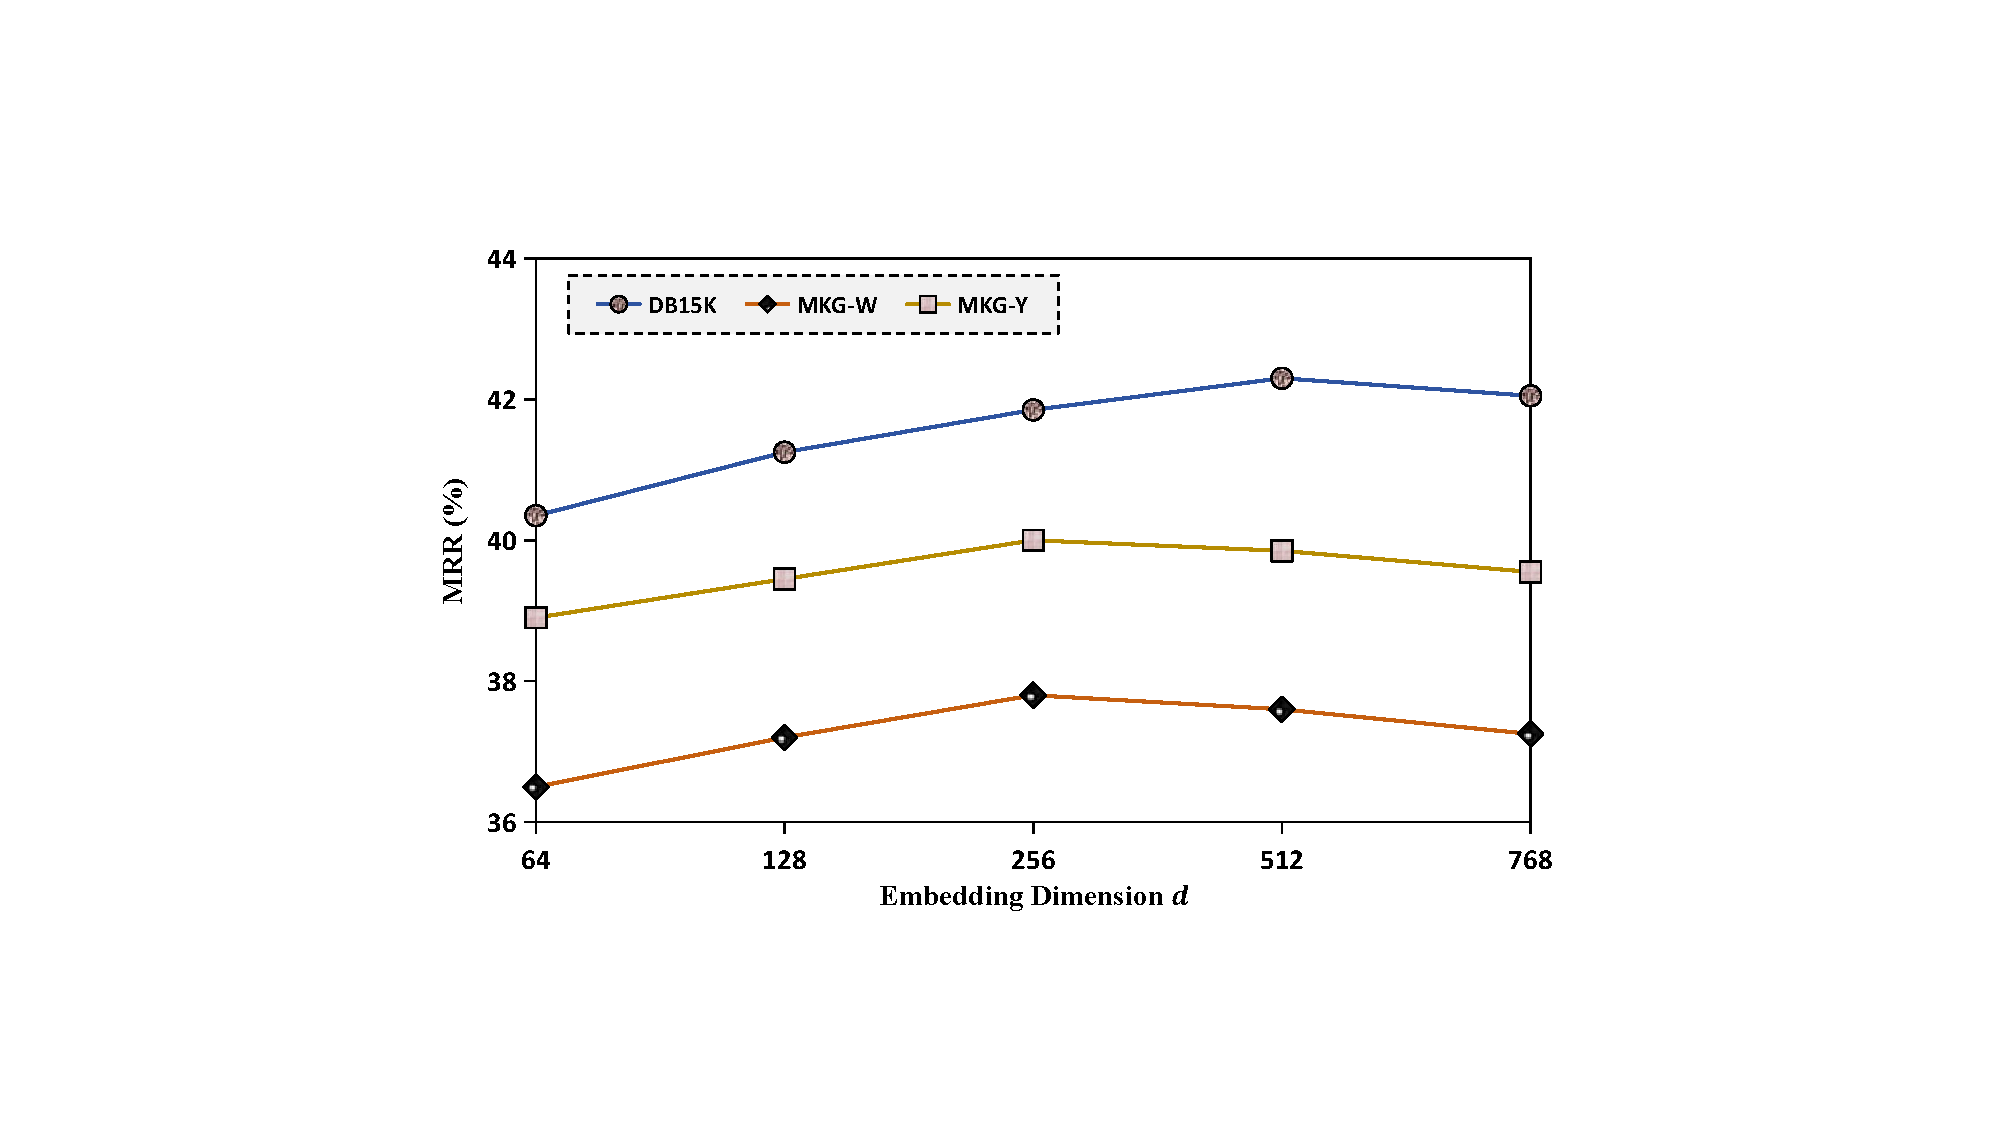
\includegraphics[width=0.3\textwidth]{sensitivity_d_equal_spacing.pdf}
    }
    \subfigure[Sensitivity to hypergraph propagation depth]{
        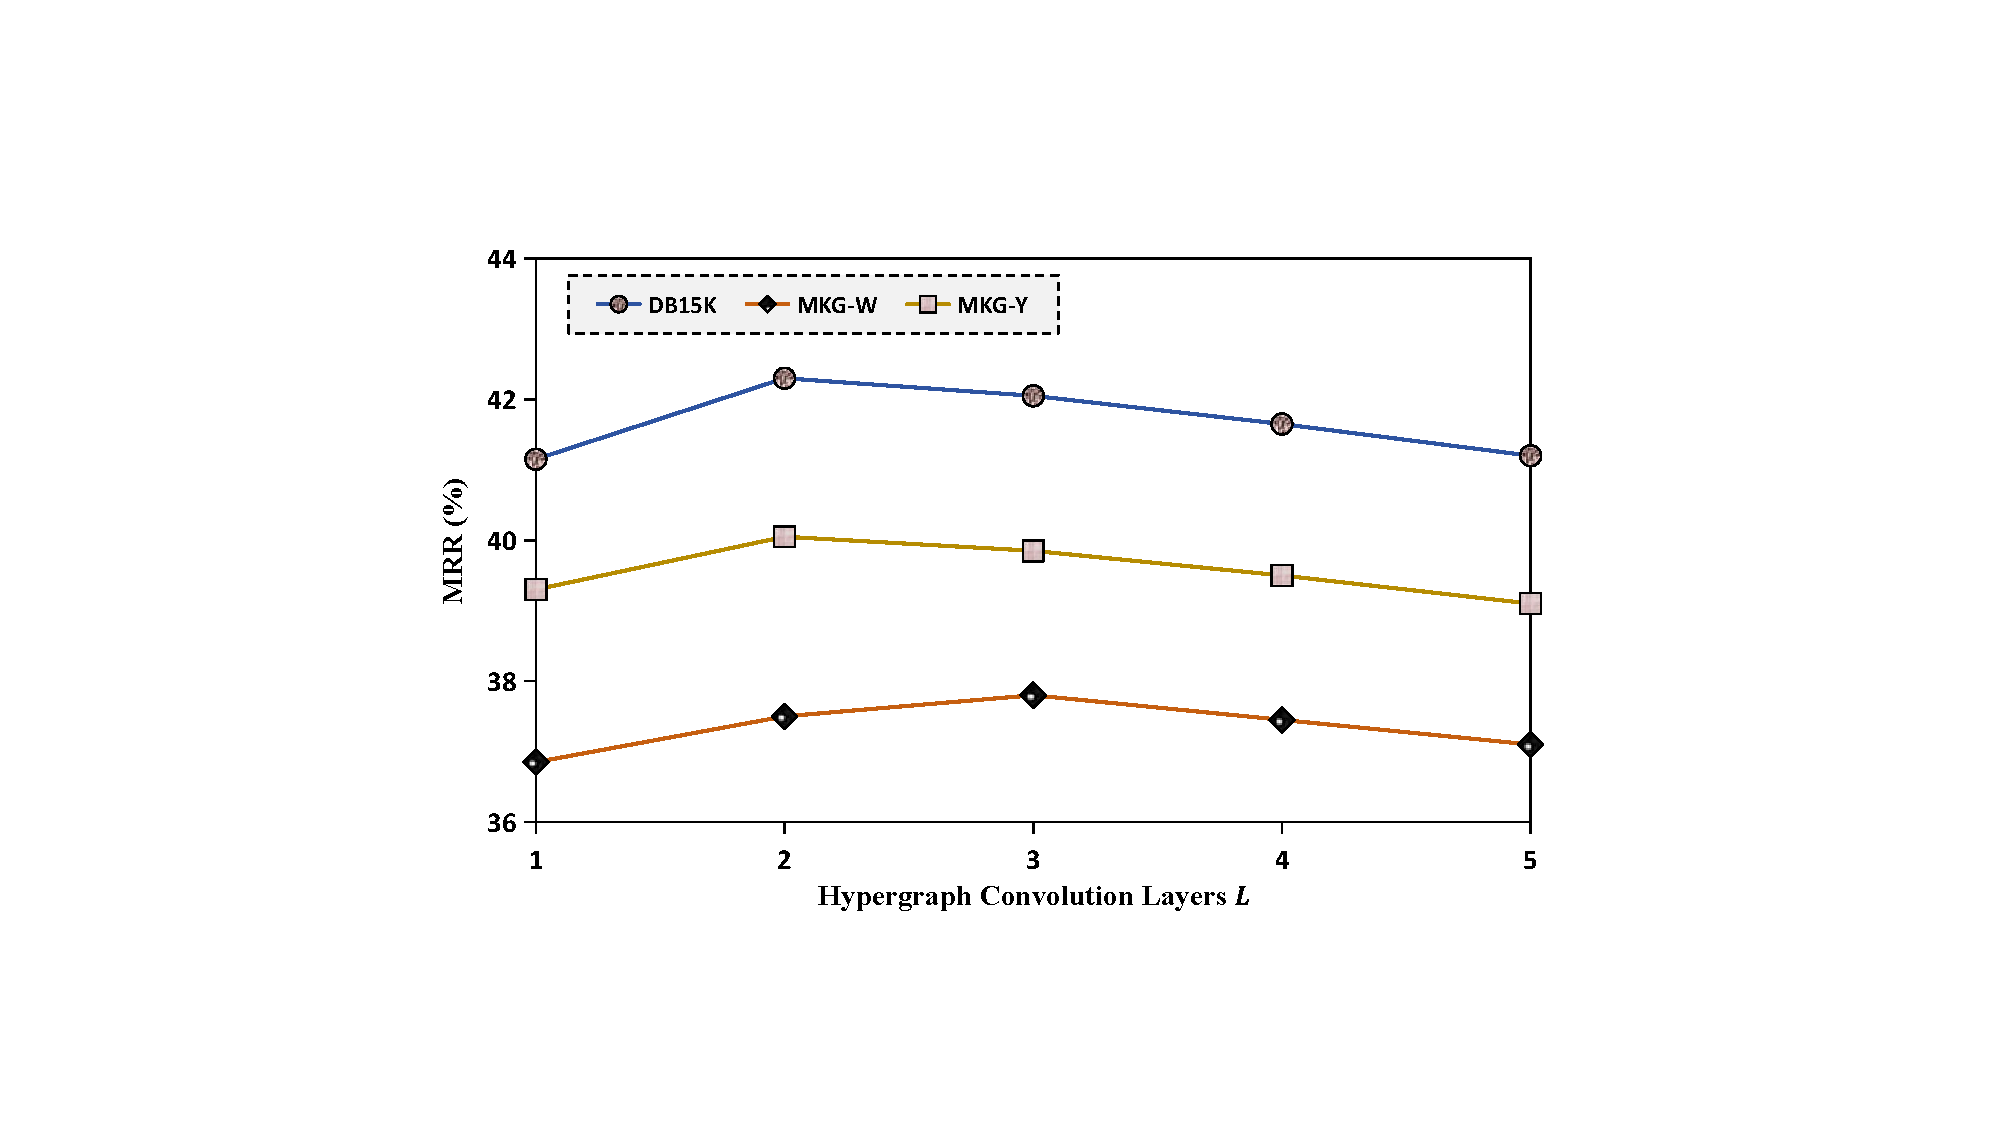
\includegraphics[width=0.3\textwidth]{sensitivity_L_equal_spacing.pdf}
    }
    \subfigure[Sensitivity to neighborhood expansion range]{
        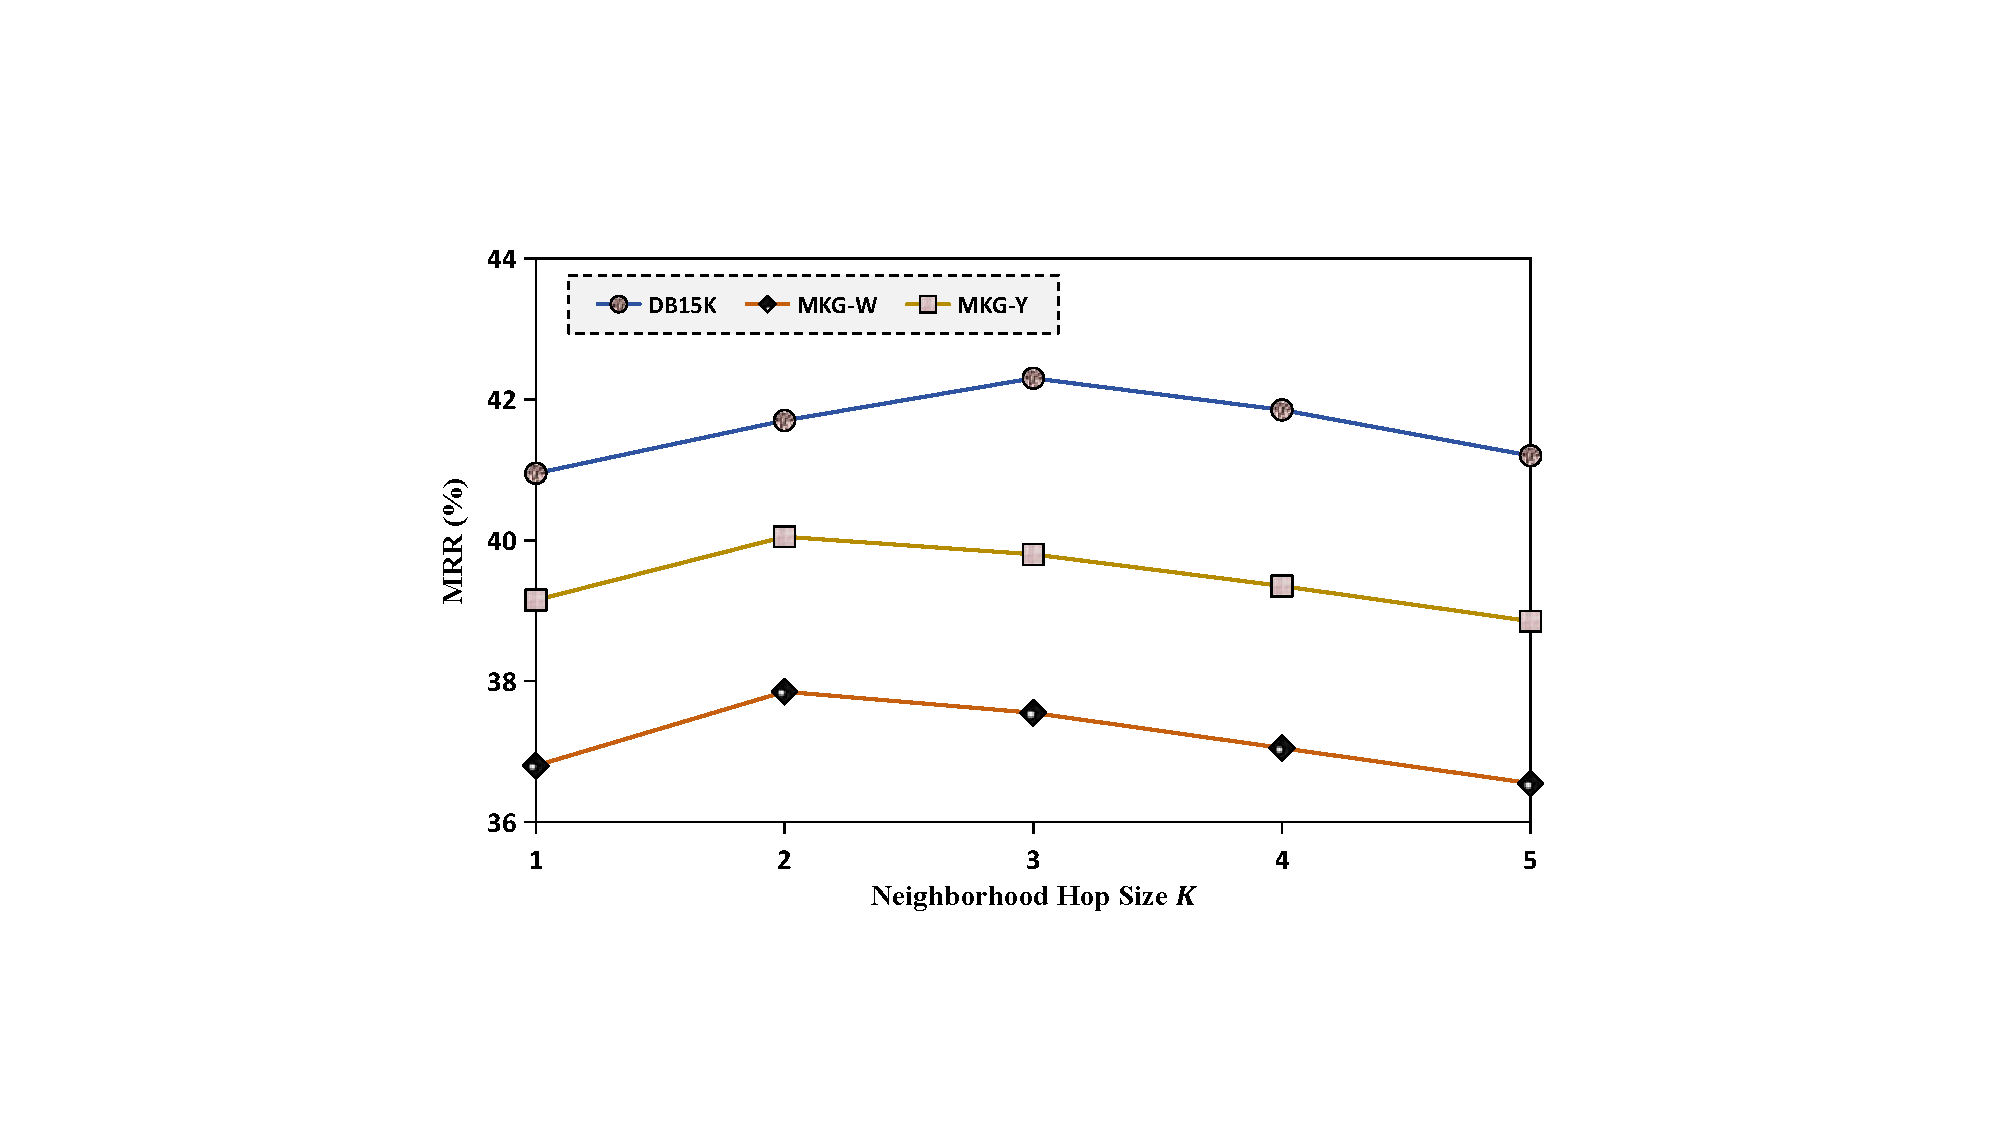
\includegraphics[width=0.3\textwidth]{sensitivity_K_equal_spacing.pdf}
    }
    \subfigure[Sensitivity to relation-relevant path number]{
        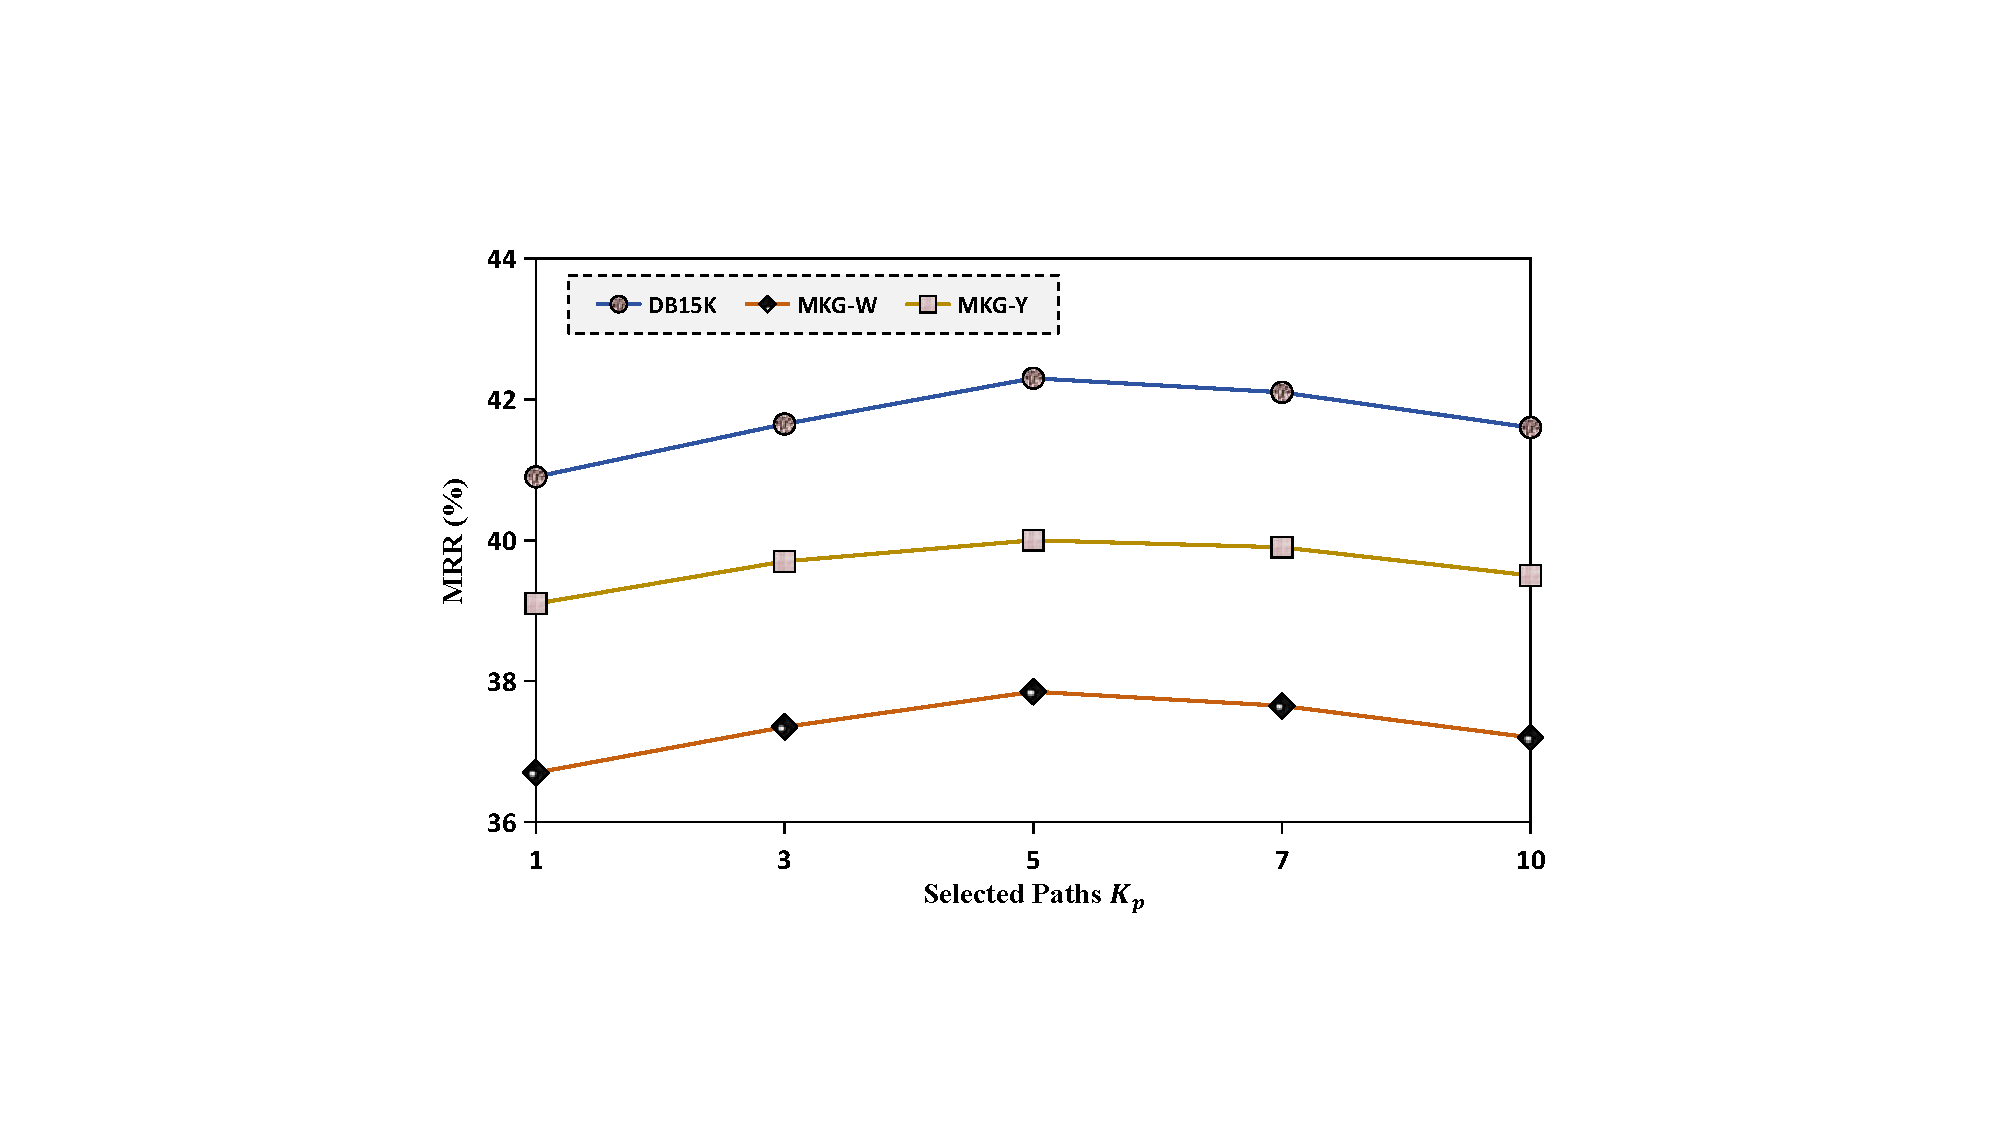
\includegraphics[width=0.3\textwidth]{sensitivity_Kp_equal_spacing.pdf}
    }
    \subfigure[Sensitivity to perturbation magnitude]{
        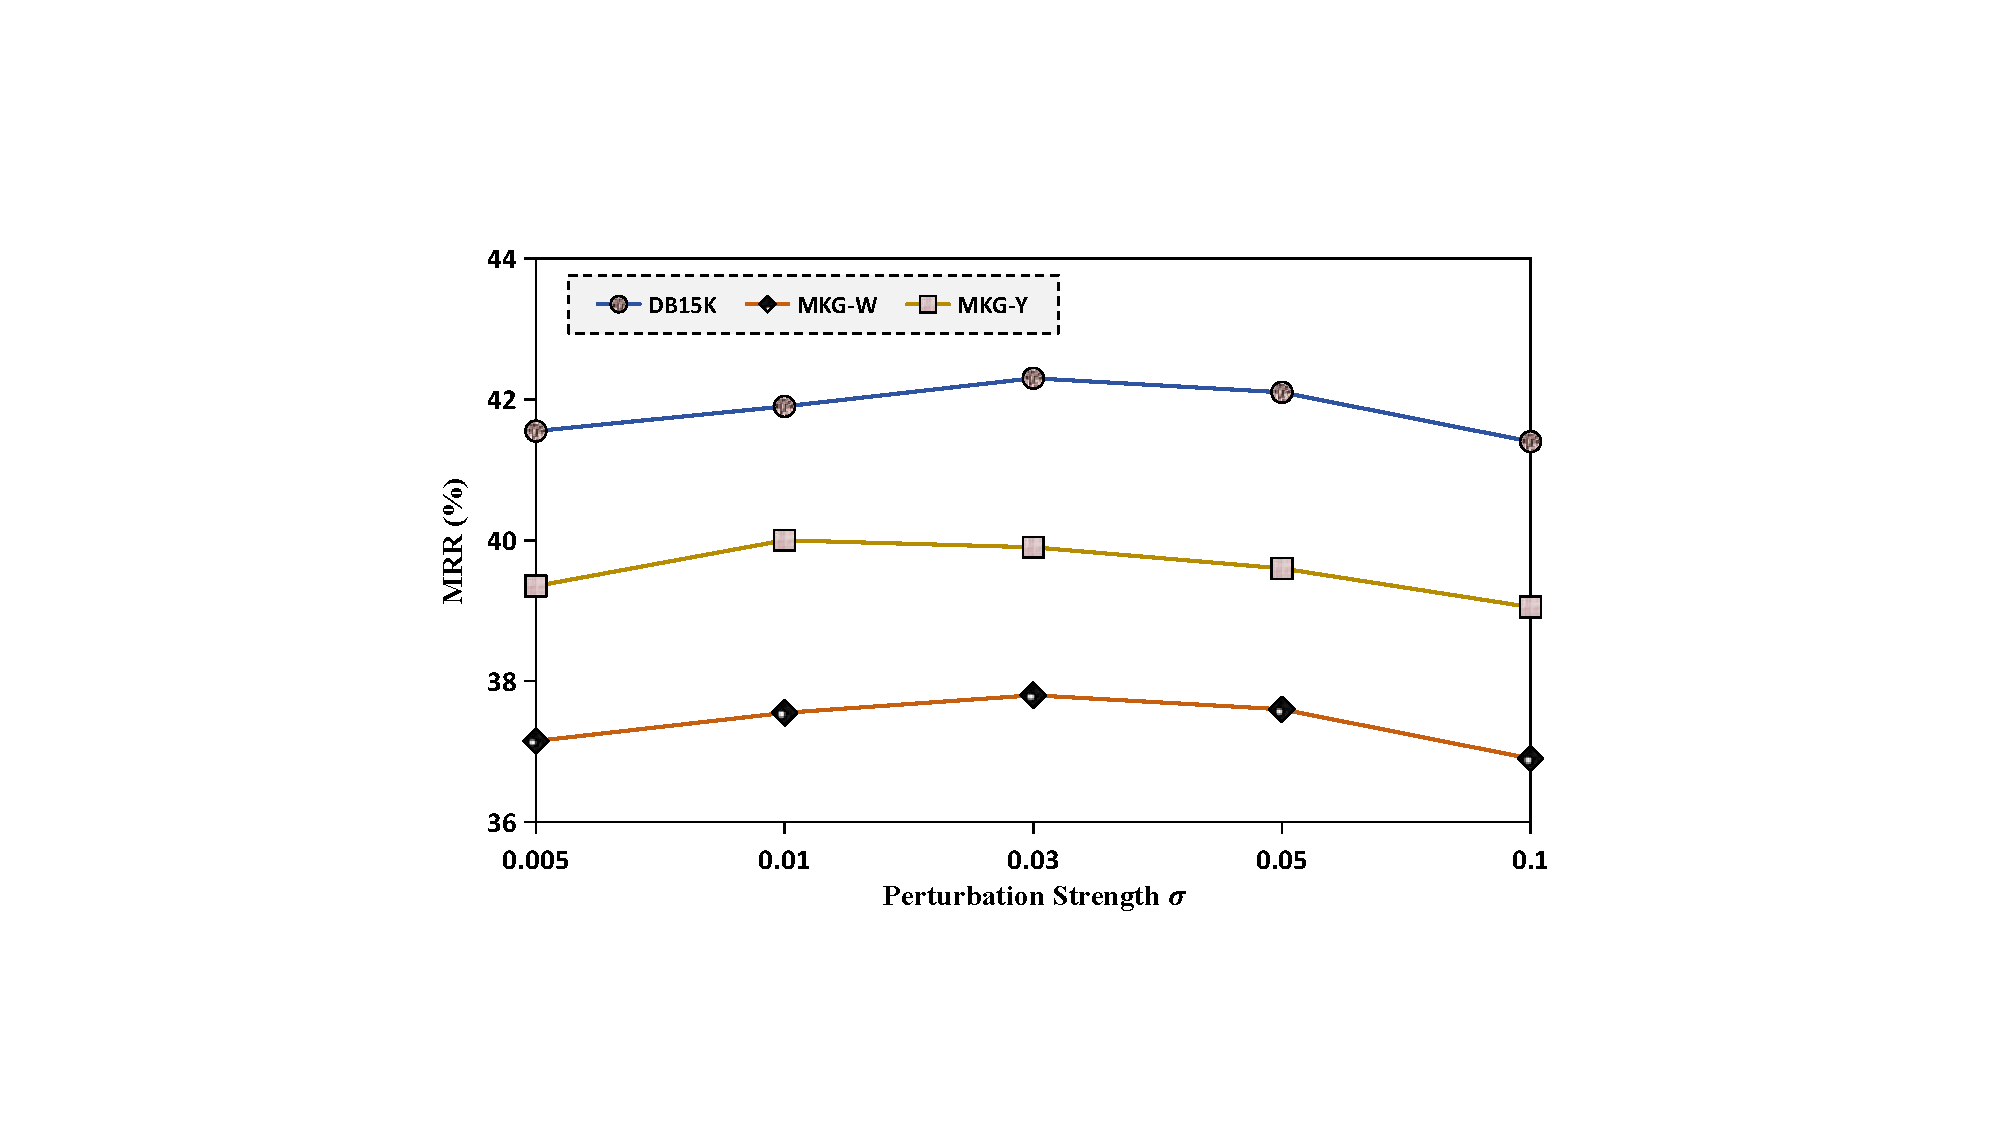
\includegraphics[width=0.3\textwidth]{sensitivity_sigma_equal_spacing.pdf}
    }
    \subfigure[Sensitivity to consistency regularization weight]{
        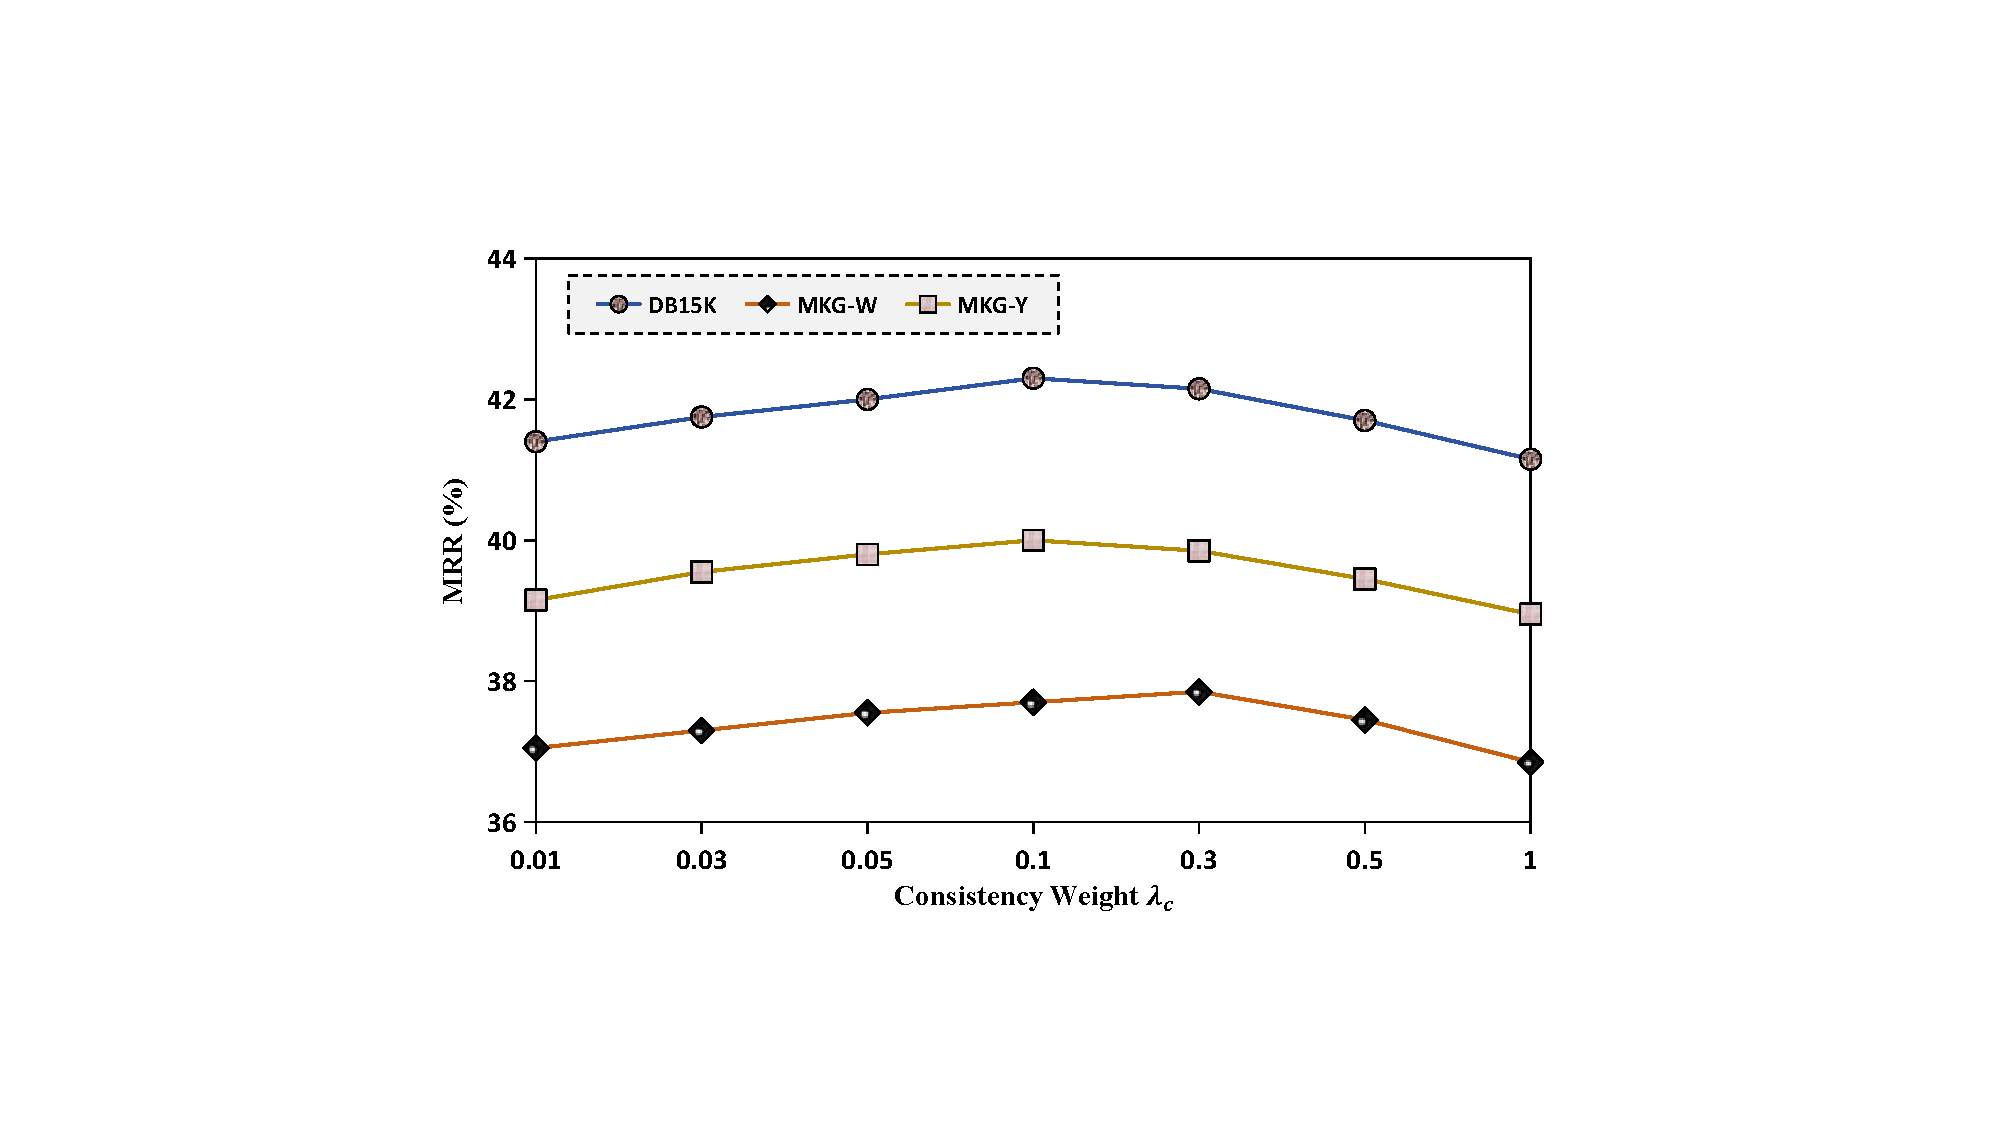
\includegraphics[width=0.3\textwidth]{sensitivity_lambdac_equal_spacing.pdf}
    }
    \caption{Parameter sensitivity analysis of HERO on DB15K, MKG-W, and MKG-Y. 
    MRR is reported under different values of six key hyperparameters. 
    HERO maintains stable performance within reasonable parameter ranges, while extreme values may weaken representation capacity, high-order structure propagation, local context construction, or perturbation consistency regularization.}
    \label{fig:parameter_sensitivity}
\end{figure*}

As shown in Figure~\ref{fig:parameter_sensitivity}, HERO is stable across broad hyperparameter ranges, although extreme settings still hurt performance. Larger embedding dimensions improve capacity at first but may overfit when too large. Moderate hypergraph depth works best, since shallow propagation underuses relation hyperedges whereas deep propagation may over-smooth entity representations. Similarly, suitable neighborhood hops and relation-relevant path numbers balance structural coverage and noise control.

The robustness-related parameters show the same pattern. Moderate perturbation strength and consistency weight improve stability, while overly weak regularization is ineffective and overly strong regularization can distort embeddings or dominate the KGC objective. The best settings vary slightly across datasets, but the overall trend supports the use of compact local contexts, moderate high-order propagation, and balanced perturbation consistency.


\subsubsection{Complexity Analysis}

To evaluate the computational cost of HERO, we analyze both its theoretical complexity and empirical efficiency. Since HERO consists of hypergraph-based multimodal pre-training, candidate-specific context-aware reasoning, and perturbation consistency optimization, its additional computational cost mainly comes from relation hypergraph convolution, local subgraph propagation, and dual-branch consistency regularization during training. We compare HERO with representative strong baselines, including MyGO, SAFER, M-Hyper, and the ablated variant HERO w/o PCRE. The empirical results are reported on DB15K, MKG-W, and MKG-Y.

\begin{table}[t]
\centering
\caption{Theoretical complexity of major components in HERO.}
\label{tab:theoretical_complexity}
\begin{tabular}{ll}
\toprule
\textbf{Component} & \textbf{Complexity} \\
\midrule
Multimodal projection & $O(|\mathcal{E}|d(d_t+d_v))$ \\
Relation hypergraph convolution & $O(L|\mathbf{H}|d + L|\mathcal{E}|d^2)$ \\
Hyperedge representation aggregation & $O(|\mathbf{H}|d)$ \\
Context-aware subgraph extraction & $O(|\mathcal{N}_{K}| + |\mathcal{P}_{\tau}|)$ \\
Relation-aware graph attention & $O(L_g|\mathcal{A}_{\tau}|d)$ \\
Perturbation consistency optimization & $O(2L_g|\mathcal{A}_{\tau}|d)$ \\
Triple scoring & $O(d)$ \\
\bottomrule
\end{tabular}
\end{table}

Table~\ref{tab:theoretical_complexity} summarizes the theoretical complexity of the major components in HERO. Here, $|\mathbf{H}|$ denotes the number of non-zero entries in the relation hypergraph incidence matrix, $L$ is the number of hypergraph convolution layers, $|\mathcal{N}_{K}|$ denotes the size of the extracted $K$-hop neighborhood, $|\mathcal{P}_{\tau}|$ denotes the number of selected relation-relevant paths for candidate triple $\tau$, $|\mathcal{A}_{\tau}|$ denotes the number of relation edges in the context-aware subgraph, and $L_g$ is the number of relation-aware graph attention layers. The perturbation consistency module introduces an additional perturbed branch during training, which approximately doubles the local propagation cost. However, this branch is only used for robustness regularization and is discarded during inference.

\begin{table*}[t]
\centering
\caption{Model size and memory consumption on three datasets. Params denotes the number of trainable parameters. GPU memory is measured during training under the same batch size setting.}
\label{tab:params_memory}
\resizebox{\textwidth}{!}{
\begin{tabular}{lccccccccc}
\toprule
\multirow{2}{*}{\textbf{Model}}
& \multicolumn{3}{c}{\textbf{DB15K}}
& \multicolumn{3}{c}{\textbf{MKG-W}}
& \multicolumn{3}{c}{\textbf{MKG-Y}} \\
\cmidrule(lr){2-4} \cmidrule(lr){5-7} \cmidrule(lr){8-10}
& Params (M) & Memory (GB) & MRR
& Params (M) & Memory (GB) & MRR
& Params (M) & Memory (GB) & MRR \\
\midrule
MyGO~\cite{zhang2025mygo}        & 18.7 & 8.6  & 37.72 & 17.9 & 7.8  & 36.10 & 16.8 & 7.1  & 38.44 \\
SAFER~\cite{li2026safer}         & 21.4 & 9.3  & 39.04 & 20.6 & 8.5  & 36.42 & 19.2 & 7.7  & 38.96 \\
M-Hyper~\cite{liu2026mhyper}     & 24.8 & 10.2 & 41.25 & 23.5 & 9.4  & 37.02 & 22.1 & 8.6  & 39.46 \\
HERO w/o PCRE                    & 26.5 & 10.7 & 40.08 & 25.2 & 9.8  & 36.58 & 23.6 & 8.9  & 39.12 \\
HERO                             & 27.3 & 12.4 & \textbf{42.31} & 25.9 & 11.2 & \textbf{37.84} & 24.3 & 10.1 & \textbf{40.03} \\
\bottomrule
\end{tabular}
}
\end{table*}

Table~\ref{tab:params_memory} reports the model size and GPU memory consumption of different methods. Compared with M-Hyper, HERO introduces a moderate increase in trainable parameters due to relation hypergraph modeling and relation-aware local reasoning. The memory consumption of HERO is also higher than that of HERO w/o PCRE during training, because PCRE performs an additional perturbed-branch propagation for consistency regularization. Nevertheless, the increase remains within a practical range. For example, on DB15K, HERO requires 12.4 GB GPU memory, which is 2.2 GB higher than M-Hyper, while improving MRR from 41.25 to 42.31. Similar trends can be observed on MKG-W and MKG-Y, indicating that the performance improvement of HERO is not achieved at the cost of excessive memory overhead.

\begin{table*}[t]
\centering
\caption{Training and inference efficiency comparison. Training time denotes the average time per epoch, and inference time denotes the average time for evaluating the test set.}
\label{tab:runtime}
\resizebox{\textwidth}{!}{
\begin{tabular}{lccccccccc}
\toprule
\multirow{2}{*}{\textbf{Model}}
& \multicolumn{3}{c}{\textbf{DB15K}}
& \multicolumn{3}{c}{\textbf{MKG-W}}
& \multicolumn{3}{c}{\textbf{MKG-Y}} \\
\cmidrule(lr){2-4} \cmidrule(lr){5-7} \cmidrule(lr){8-10}
& Train (s/epoch) & Inference (s) & MRR
& Train (s/epoch) & Inference (s) & MRR
& Train (s/epoch) & Inference (s) & MRR \\
\midrule
MyGO~\cite{zhang2025mygo}        & 42.6 & 18.4 & 37.72 & 31.8 & 13.6 & 36.10 & 24.5 & 10.8 & 38.44 \\
SAFER~\cite{li2026safer}         & 51.3 & 21.7 & 39.04 & 38.6 & 16.2 & 36.42 & 29.4 & 12.7 & 38.96 \\
M-Hyper~\cite{liu2026mhyper}     & 57.8 & 24.3 & 41.25 & 43.1 & 18.6 & 37.02 & 33.7 & 14.1 & 39.46 \\
HERO w/o PCRE                    & 63.5 & 26.1 & 40.08 & 47.2 & 19.9 & 36.58 & 36.4 & 15.2 & 39.12 \\
HERO                             & 74.9 & 26.8 & \textbf{42.31} & 55.6 & 20.4 & \textbf{37.84} & 42.1 & 15.7 & \textbf{40.03} \\
\bottomrule
\end{tabular}
}
\end{table*}

Table~\ref{tab:runtime} presents the empirical runtime comparison. HERO requires more training time because it jointly optimizes relation hypergraph pre-training, candidate-specific local reasoning, and perturbation consistency. Compared with HERO w/o PCRE, training time increases by 11.4, 8.4, and 5.7 seconds per epoch on DB15K, MKG-W, and MKG-Y, respectively. The extra cost mainly comes from the perturbed branch, which is removed during evaluation; therefore, inference time remains close to HERO w/o PCRE.
The runtime differences across datasets are also consistent with their structural characteristics. DB15K contains more relation types and training triples, resulting in higher costs for relation hypergraph construction and candidate-specific local reasoning. MKG-W contains a relatively large entity set but fewer triples than DB15K, leading to moderate runtime. MKG-Y has fewer relation types and structural triples, and therefore requires less training and inference time. These observations suggest that the computational cost of HERO is mainly affected by the scale of structural triples, relation distribution, and the size of candidate-specific subgraphs.

The complexity analysis indicates a practical trade-off between effectiveness and efficiency. Relation hypergraph modeling and perturbation consistency introduce additional training overhead, but inference remains comparable to strong baselines. The higher MRR across datasets suggests that this extra computation is used for relation-level high-order modeling, candidate-specific local reasoning, and robust prediction.


\subsubsection{Case Study}

The case study on DB15K examines both reasoning behavior and representation quality. Representative test queries are used to compare HERO with M-Hyper, and t-SNE visualization is applied to entity embeddings to inspect relation-discriminative structure. The examples cover \textit{recordLabel}, \textit{genre}, \textit{starring}, \textit{birthPlace}, \textit{instrument}, and \textit{country}, involving music-, film-, person-, and location-related semantics.

\begin{table*}[t]
\centering
\caption{Case study on DB15K. The sampled queries are from the test set, and the supporting contexts are extracted from the training graph. Lower rank indicates better prediction.}
\label{tab:case_study}
\renewcommand{\arraystretch}{1.18}
\setlength{\tabcolsep}{4.5pt}
\resizebox{\textwidth}{!}{
\begin{tabular}{p{3.2cm}p{2.2cm}ccp{6.2cm}}
\toprule
\textbf{Query} 
& \textbf{Ground Truth} 
& \textbf{M-Hyper} 
& \textbf{HERO} 
& \textbf{Representative Supporting Context} \\
\midrule

\textit{Matt Bellamy} \newline 
$\xrightarrow{\textit{recordLabel}}$ ? 
& East West Records
& 3 
& \textbf{1}
& \textit{Matt Bellamy} $\xrightarrow{\textit{associatedBand}}$ \textit{Muse} 
$\xrightarrow{\textit{recordLabel}}$ \textit{East West Records} \\

\midrule

\textit{Steve Jordan} \newline 
$\xrightarrow{\textit{genre}}$ ? 
& Jazz
& 3 
& \textbf{1}
& \textit{Steve Jordan} $\xrightarrow{\textit{genre}}$ \textit{Blues} 
$\xrightarrow{\textit{derivative}}$ \textit{Jazz} \\

\midrule

\textit{Skate punk} \newline 
$\xrightarrow{\textit{instrument}}$ ? 
& Drum kit
& 3 
& \textbf{1}
& \textit{Skate punk} $\xrightarrow{\textit{stylisticOrigin}}$ \textit{Melodic hardcore} 
$\xrightarrow{\textit{instrument}}$ \textit{Drum kit} \\

\midrule

\textit{Superbad} \newline 
$\xrightarrow{\textit{starring}}$ ? 
& Seth Rogen
& 3 
& \textbf{1}
& \textit{Superbad} $\xrightarrow{\textit{writer}}$ \textit{Seth Rogen}; 
\textit{50/50} $\xrightarrow{\textit{starring}}$ \textit{Seth Rogen} \\

\midrule

\textit{Aldo Nova} \newline 
$\xrightarrow{\textit{birthPlace}}$ ? 
& Canada
& 3 
& \textbf{1}
& \textit{Aldo Nova} $\xrightarrow{\textit{birthPlace}}$ \textit{Montreal} 
$\xrightarrow{\textit{country}}$ \textit{Canada} \\

\midrule

\textit{Earth, Wind \& Fire} \newline 
$\xrightarrow{\textit{genre}}$ ? 
& Psychedelic soul
& 3 
& \textbf{1}
& \textit{Earth, Wind \& Fire} $\xrightarrow{\textit{genre}}$ \textit{Soul music} 
$\xrightarrow{\textit{musicFusionGenre}}$ \textit{Psychedelic soul} \\

\bottomrule
\end{tabular}
}
\end{table*}

Table~\ref{tab:case_study} reports representative prediction cases on DB15K. For each query, the ground-truth entity comes from the test set, while the supporting context is extracted from the training graph. Compared with M-Hyper, HERO ranks the correct entity higher in all sampled cases, indicating that HERO can better exploit candidate-specific structural evidence rather than relying only on global multimodal representations. For example, in the query $(\mathrm{Matt\ Bellamy}, \mathrm{recordLabel}, ?)$, the training graph contains a relation-relevant path connecting \textit{Matt Bellamy} to \textit{East West Records} through \textit{Muse}. Such local structural context provides useful evidence for identifying the correct record label. Similarly, in the genre and instrument prediction cases, relation compositions such as \textit{stylisticOrigin}, \textit{derivative}, and \textit{musicFusionGenre} provide additional structural cues for candidate ranking.

\begin{figure*}[t]
    \centering
    \subfigure[t-SNE visualization of M-Hyper]{
        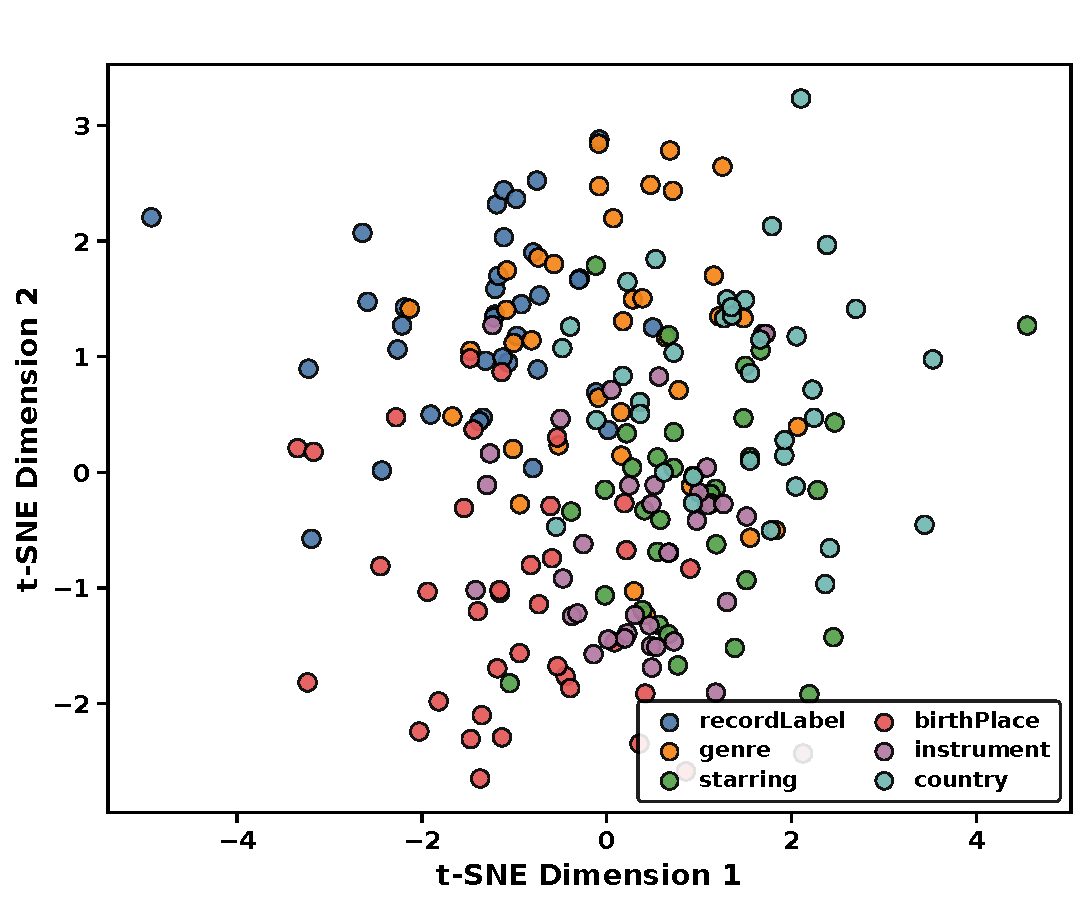
\includegraphics[width=0.3\textwidth]{tsne_mhyper.pdf}
    }
    \subfigure[t-SNE visualization of HERO w/o RAGAN]{
        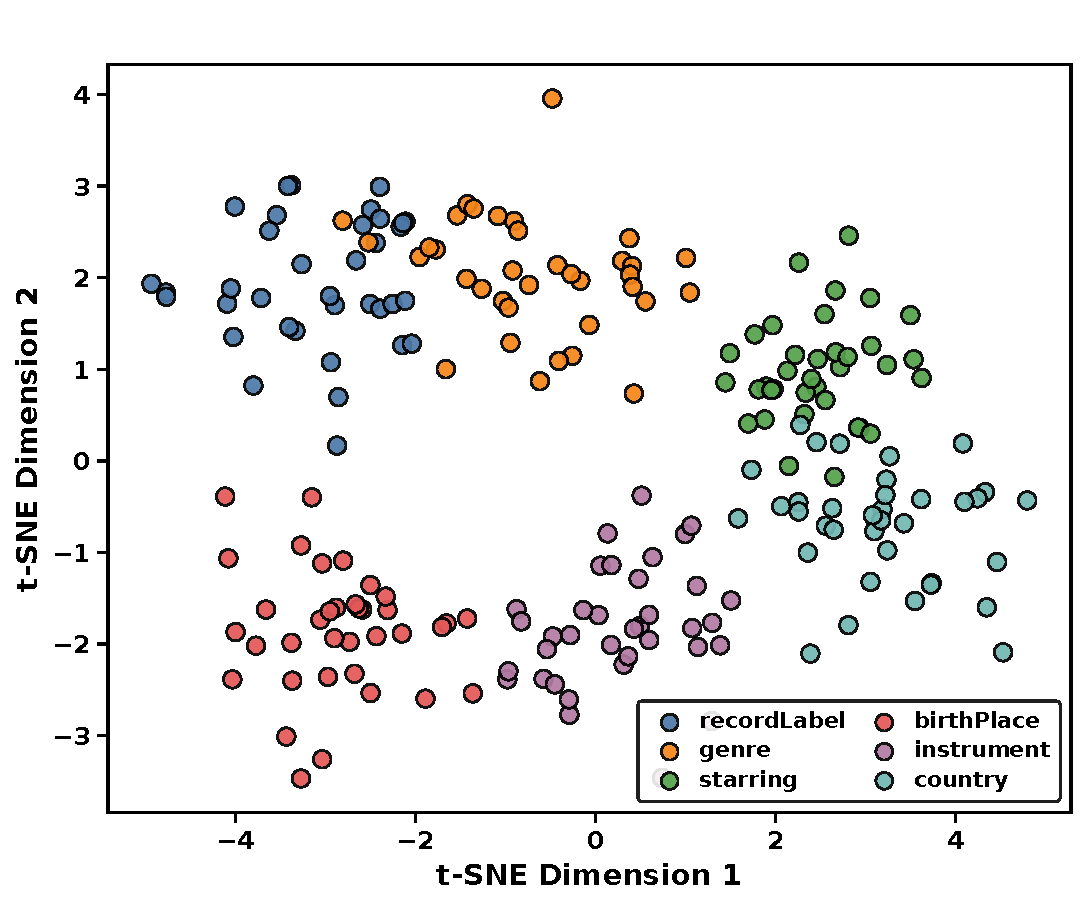
\includegraphics[width=0.3\textwidth]{tsne_hero_wo_ragan.pdf}
    }
    \subfigure[t-SNE visualization of HERO]{
        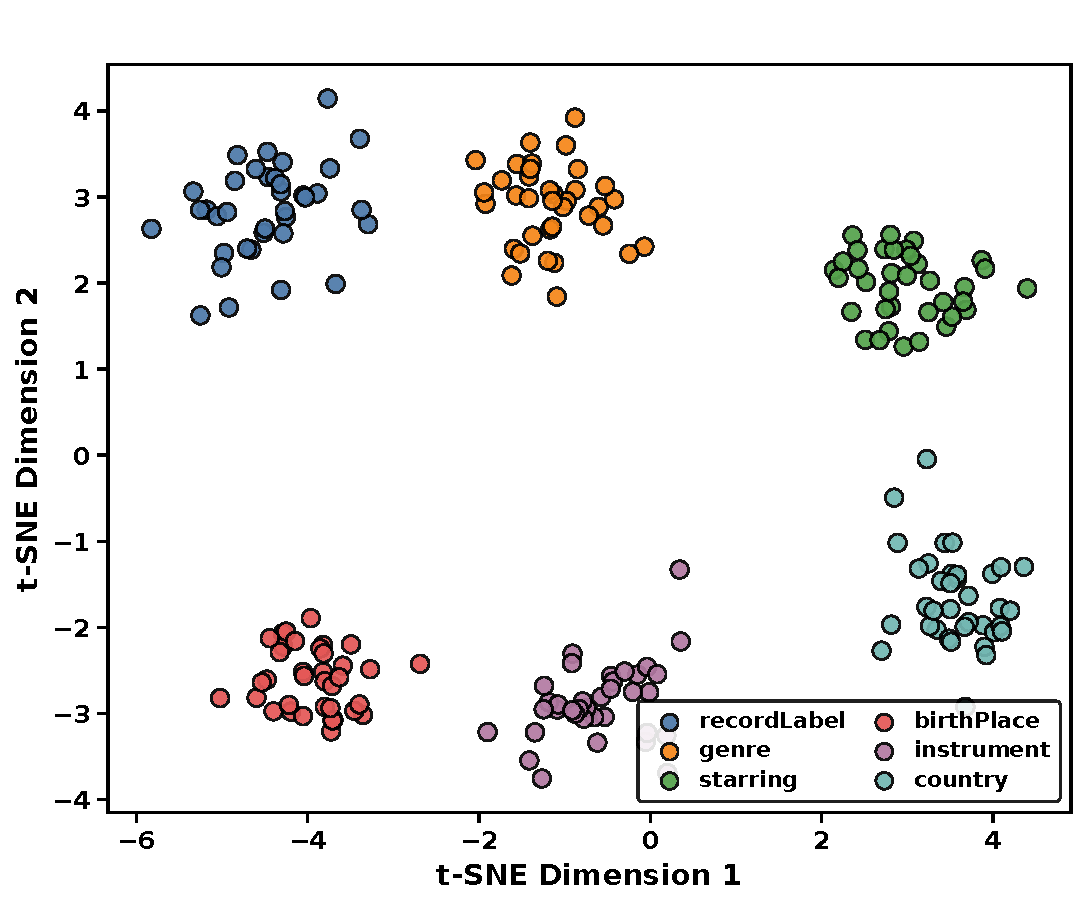
\includegraphics[width=0.3\textwidth]{tsne_hero.pdf}
    }
    \caption{t-SNE visualization of entity embeddings on DB15K. 
    Entities are sampled from representative relation categories and colored according to their dominant relation types. 
    Compared with M-Hyper and HERO w/o RAGAN, HERO produces more compact intra-relation clusters and clearer inter-relation separation, indicating stronger relation-aware representation learning.}
    \label{fig:tsne_case_study}
\end{figure*}

Although the sampled cases illustrate the reasoning behavior of HERO at the instance level, they do not fully reflect the structure of the learned representation space. Therefore, we further visualize the entity embeddings learned by different methods. Specifically, entities associated with the relation categories used in Table~\ref{tab:case_study} are sampled and projected into a two-dimensional space using t-SNE. This visualization connects instance-level ranking behavior with global representation separability, providing a more comprehensive qualitative analysis of HERO.

Figure~\ref{fig:tsne_case_study} presents the visualization results of three representation spaces. As shown in Figure~\ref{fig:tsne_case_study}(a), the embeddings produced by M-Hyper exhibit substantial overlap among different relation categories. Although M-Hyper improves multimodal representation learning by preserving both fused and modality-specific information, its representation space is still mainly shaped by global multimodal fusion and pairwise triple scoring. As a result, entities associated with semantically adjacent relations, such as \textit{genre}, \textit{instrument}, and \textit{recordLabel}, are not clearly separated.

Figure~\ref{fig:tsne_case_study}(b) presents the representation distribution of HERO w/o RAGAN. Compared with M-Hyper, the clusters become more structured, suggesting that relation hypergraph pre-training improves relation-level organization. By transforming pairwise triples into relation-specific hyperedges, HERO w/o RAGAN allows entities sharing similar relation semantics to exchange information through high-order structural propagation. This makes the learned embeddings more coherent within relation categories. Nevertheless, partial overlap still exists among several relation groups, since this variant does not incorporate candidate-specific local reasoning during triple prediction. The complete HERO model in Figure~\ref{fig:tsne_case_study}(c) yields the most compact and separable embedding distribution. Entities belonging to the same relation category are grouped more closely, while different relation categories show clearer boundaries. This visualization suggests that candidate-specific context-aware reasoning further refines relation-aware representations by incorporating dual-end neighborhoods and relation-relevant multi-hop paths. In addition, perturbation consistency optimization stabilizes the representation space by reducing the influence of noisy multimodal signals and weakly related structural contexts.

Table~\ref{tab:case_study} and Figure~\ref{fig:tsne_case_study} give complementary qualitative evidence. The ranking cases show that HERO identifies ground-truth entities more reliably for specific queries, while the t-SNE results show a more relation-discriminative embedding space. These findings align with the quantitative results: relation hypergraph modeling improves high-order structural representation, candidate-specific reasoning strengthens local discrimination, and perturbation consistency stabilizes the learned representations.

\section{Conclusion}
\label{sec:conclusion}
This paper presented HERO, a hypergraph-enhanced relation-aware robust reasoning framework for multimodal knowledge graph completion. The framework targets two limitations of existing MMKGC methods: insufficient modeling of relation-level high-order dependencies under pairwise structures, and unstable prediction under noisy multimodal and structural conditions. HERO converts each relation type into a relation-specific hyperedge, performs candidate-specific reasoning with dual-end neighborhoods and relation-relevant paths, and applies embedding- and score-level perturbation consistency for stable ranking. Experiments on multiple MMKGC benchmarks show consistent improvements over strong baselines, and the ablation, robustness, sensitivity, complexity, and case analyses support the contribution of each component.

Several limitations remain. HERO is evaluated mainly in a transductive and relatively static setting, while real MMKGs may evolve with new entities, relations, images, and descriptions. Extending HERO to inductive, dynamic, or incremental scenarios is therefore important. The current model also focuses on textual and visual modalities; richer signals such as audio, video, and temporal information may provide additional evidence but require stable cross-modal reasoning. Finally, candidate-specific subgraph construction and dual-branch robustness training increase training cost. More efficient subgraph sampling, path selection, and lightweight regularization could improve scalability, and the same ideas may also benefit multimodal entity alignment, knowledge graph question answering, and multi-hop reasoning.



% To print the credit authorship contribution details
\section*{Declaration of competing interest}
The authors declare that they have no known competing financial
interests or personal relationships that could have appeared to influence
the work reported in this paper.


\section*{Acknowledgements}
This work was supported by Science and Technology Research Project of Henan Province (grant no. 262102211055).

\bibliography{aej-refs}

\end{document}
